\documentclass[12pt,a4paper]{report}

% ==============================================================================
% GCTU FACULTY OF ENGINEERING MARGIN SPECIFICATIONS
% Top: 2.5 cm; Bottom: 2.5 cm; Left: 4.0 cm (for binding); Right: 2.5 cm
% ==============================================================================
\usepackage[top=2.5cm, bottom=2.5cm, left=4.0cm, right=2.5cm]{geometry}

% ================= TYPOGRAPHY & SPACING =================
\usepackage{setspace}
\onehalfspacing % 1.5 line spacing per GCTU handbook

% Paragraphing: First line must NOT be indented; paragraphs line-spaced
\setlength{\parindent}{0pt}
\setlength{\parskip}{1em}

% ================= CORE PACKAGES =================
\usepackage{graphicx}
\graphicspath{{figures/}} % Self-contained figure search path (Overleaf compliant)
\usepackage{amsmath,amssymb,amsfonts}
\usepackage{booktabs,array,ragged2e,longtable,pdflscape,float}
\usepackage{url}
\usepackage{cite}
\usepackage{xcolor}
\usepackage[hidelinks]{hyperref}

% Table caption above, figure caption below (Handbook Section 2.3)
\usepackage[tableposition=top,figureposition=bottom]{caption}

\begin{document}

% ==============================================================================
% PRELIMINARY PAGES (ROMAN NUMERALS ii, iii, iv...)
% ==============================================================================
\pagenumbering{roman}
\pagestyle{plain}

% 1. Title Page (Page i - number omitted per Handbook)
% ==============================================================================
% TITLE PAGE — GCTU FACULTY OF ENGINEERING SPECIFICATION
% ==============================================================================
\begin{titlepage}
\begin{center}

{\fontsize{16pt}{20pt}\bfseries GHANA COMMUNICATION TECHNOLOGY UNIVERSITY (GCTU)\par}
\vspace{0.8cm}
{\fontsize{14pt}{18pt}\bfseries FACULTY OF ENGINEERING\par}
\vspace{0.5cm}
{\fontsize{13pt}{16pt}\bfseries DEPARTMENT OF COMPUTER ENGINEERING\par}

\vspace{1.5cm}


\includegraphics[width=3.5cm]{gctu_logo.png}\par
\vspace{0.8cm}

{\fontsize{15pt}{20pt}\bfseries DEVELOPMENT AND IMPLEMENTATION OF A ROBOTIC APPLICATION FOR HUMAN INTENTION RECOGNITION USING MOTION AND HAND GESTURE\par}

\vspace{1.5cm}

{\fontsize{12pt}{16pt}\itshape A Project Work Submitted in Partial Fulfillment of the Requirements for the Award of the Degree of\par}
\vspace{0.3cm}
{\fontsize{13pt}{17pt}\bfseries BACHELOR OF SCIENCE IN COMPUTER ENGINEERING\par}

\vspace{1.8cm}

{\fontsize{12pt}{15pt}\textbf{BY:}\par}
\vspace{0.3cm}
{\fontsize{12pt}{16pt}
\begin{tabular}{cc}
\textbf{ELEANA OSEI OWUSU} & (Index No.: 4121230024) \\
\textbf{JOEL NII ADJETEY AHULU} & (Index No.: 4121230020) \\
\end{tabular}\par
}

\vfill

{\fontsize{12pt}{15pt}\textbf{SUPERVISOR:}\par}
\vspace{0.2cm}
{\fontsize{12pt}{15pt}\textbf{MR. MICHEAL XENYA}\par}

\vspace{1.0cm}

{\fontsize{12pt}{15pt}\textbf{SEPTEMBER, 2026}\par}

\end{center}
\end{titlepage}

\setcounter{page}{2}

% 2. Declaration & Certification
\clearpage
% ==============================================================================
% DECLARATION & CERTIFICATION — GCTU FACULTY OF ENGINEERING SPECIFICATION
% ==============================================================================
\chapter*{DECLARATION}
\addcontentsline{toc}{chapter}{DECLARATION}

\section*{Candidate's Declaration}
This project is presented as part of the requirements for the award of the Degree of \textbf{Bachelor of Science in Computer Engineering} by Ghana Communication Technology University. We hereby declare that this project report is entirely the result of our own original research, hardware implementation, and empirical inquiries. We affirm that this project work has not been presented, in whole or in part, for the award of any other diploma or degree in this university or elsewhere. All sources of scholarly information, technical libraries, and literature have been duly cited and acknowledged.

\vspace{1.5cm}

\noindent
\begin{tabular}{p{7.5cm}p{7.5cm}}
\textbf{Eleana Osei Owusu} & \textbf{Signature:} \hrulefill \\[0.2cm]
(Index No.: 4121230024) & \textbf{Date:} \hrulefill \\[1.2cm]
\textbf{Joel Nii Adjetey Ahulu} & \textbf{Signature:} \hrulefill \\[0.2cm]
(Index No.: 4121230020) & \textbf{Date:} \hrulefill \\
\end{tabular}

\vspace{2.0cm}

\section*{Supervisor's Certification}
I hereby certify that this project work was carried out under my direct supervision in the Department of Computer Engineering, Faculty of Engineering, Ghana Communication Technology University, in partial fulfillment of the requirements for the award of the Degree of Bachelor of Science in Computer Engineering.

\vspace{1.5cm}

\noindent
\begin{tabular}{p{7.5cm}p{7.5cm}}
\textbf{Mr. Micheal Xenya} & \textbf{Signature:} \hrulefill \\[0.2cm]
(Project Supervisor) & \textbf{Date:} \hrulefill \\
\end{tabular}

\vspace{1.8cm}

\section*{Head of Department's Endorsement}
I hereby confirm that this project work has been formally examined and accepted in satisfaction of the project requirements for the Department of Computer Engineering.

\vspace{1.5cm}

\noindent
\begin{tabular}{p{7.5cm}p{7.5cm}}
\textbf{Dr. Samuel Danso} & \textbf{Signature:} \hrulefill \\[0.2cm]
(Head of Department) & \textbf{Date:} \hrulefill \\
Department of Computer Engineering & \\
\end{tabular}


% 3. Abstract
\clearpage
% ==============================================================================
% ABSTRACT — GCTU FACULTY OF ENGINEERING SPECIFICATION
% One single cohesive paragraph between 150 and 250 words.
% ==============================================================================
\chapter*{ABSTRACT}
\addcontentsline{toc}{chapter}{ABSTRACT}

Deploying intuitive touchless human-robot interaction on resource-constrained mobile robots remains severely challenged by heavy GPU compute demands, network latencies inherent in cloud offloading, and the lack of physical spatial grounding in dynamic shared workspaces. This project presents the design, physical integration, and empirical evaluation of an autonomous mobile robot cognitive framework capable of real-time human intention recognition using skeletal motion and hand gestures executed entirely on embedded edge hardware. The physical testbed integrates an 8GB Raspberry Pi 5 single-board computer, a Yahboom micro-ROS ESP32-S3 motor controller, a 2D Time-of-Flight LiDAR, and a 2-DOF pan-tilt camera gimbal. The vision pipeline throttles camera intake to 20~Hz, enforces an empirical spatial acceptance zone to reject background bystanders, extracts 21 hand landmarks, and maps them into a 19-dimensional position- and scale-invariant geometric feature vector classified by a Multilayer Perceptron (MLP). A Long Short-Term Memory (LSTM) network anticipates human walking trajectories over an 8-frame horizon, while a supervisory finite state machine arbitrates motion commands via a ROS~2 priority multiplexer alongside 2D metric SLAM and Nav2 autonomous waypoint navigation. Rigorous physical trials across 180 experimental runs achieve a 99.38\% offline test accuracy and a 96.67\% physical operational accuracy across varying illumination and operator distances up to 2.5~meters. The total measured vision-to-actuation latency of 132.0~ms satisfies the 150~ms real-time latency deadline and complies with ISO 15066:2016 collaborative robot safety standards by executing immediate reactive halt preemption at a 0.36~meter LiDAR safety boundary.

\vspace{0.8cm}
\noindent\textbf{Keywords:} Human-Robot Interaction (HRI), Autonomous Mobile Robots, Edge Computing, Hand Gesture Recognition, ROS 2 Humble, Geometric Feature Invariance, Collaborative Safety (ISO 15066).


% 4. Dedication
\clearpage
% ==============================================================================
% DEDICATION — GCTU FACULTY OF ENGINEERING SPECIFICATION
% ==============================================================================
\chapter*{DEDICATION}
\addcontentsline{toc}{chapter}{DEDICATION}

This engineering project is wholeheartedly dedicated to our beloved parents and families, whose persistent prayers, profound sacrifices, and unwavering moral and financial support provided the bedrock upon which our academic aspirations were realized. Their boundless encouragement inspired us to persevere through demanding nights of laboratory experimentation, code debugging, and hardware fabrication. 

We also dedicate this work to the prospective cohorts of computer engineering and robotics students at Ghana Communication Technology University, with the sincere hope that this open-source architecture and physical testbed serve as a practical foundation for groundbreaking advancements in autonomous systems, intelligent machines, and edge-native collaborative robotics across the African continent.


% 5. Acknowledgements
\clearpage
% ==============================================================================
% ACKNOWLEDGEMENTS — GCTU FACULTY OF ENGINEERING SPECIFICATION
% ==============================================================================
\chapter*{ACKNOWLEDGEMENTS}
\addcontentsline{toc}{chapter}{ACKNOWLEDGEMENTS}

First and foremost, we give all glory, honor, and praise to the Almighty God for granting us divine wisdom, good health, endurance, and perseverance throughout the duration of this undergraduate engineering degree program and the successful completion of this project.

We register our profound gratitude and esteem to our project supervisor, \textbf{Mr. Micheal Xenya}, for his exceptional technical mentorship, critical reviews, and unwavering guidance. His meticulous attention to rigorous engineering design, standard-compliant methodology, and persistent encouragement challenged us to surpass surface-level simulations and realize a physically validated autonomous mobile robot.

We extend our sincere appreciation to the Head of Department, faculty members, laboratory technicians, and teaching assistants in the Department of Computer Engineering, Faculty of Engineering at Ghana Communication Technology University. Their academic instruction, provision of laboratory infrastructure, and administrative support enriched our academic experience.

Our heartfelt thanks go to the student volunteers and colleagues who patiently dedicated their time to participate in the 180 physical human interaction trials and gesture recognition experiments, providing the vital empirical dataset for our quantitative evaluations. Finally, we express our endless gratitude to our families and friends for their constant emotional support, patience, and encouragement throughout this journey.


% 6. Table of Contents
\clearpage
\tableofcontents
\addcontentsline{toc}{chapter}{TABLE OF CONTENTS}

% 7. List of Tables
\clearpage
\listoftables
\addcontentsline{toc}{chapter}{LIST OF TABLES}

% 8. List of Figures
\clearpage
\listoffigures
\addcontentsline{toc}{chapter}{LIST OF FIGURES}

% 9. List of Abbreviations and Acronyms
\clearpage
% ==============================================================================
% LIST OF ABBREVIATIONS & ACRONYMS — GCTU FACULTY OF ENGINEERING SPECIFICATION
% ==============================================================================
\chapter*{LIST OF ABBREVIATIONS AND ACRONYMS}
\addcontentsline{toc}{chapter}{LIST OF ABBREVIATIONS AND ACRONYMS}

\begin{longtable}{p{3.0cm}p{12.0cm}}
\toprule
\textbf{Abbreviation} & \textbf{Full Definition / Expansion} \\
\midrule
\endhead
\textbf{ADE} & Average Displacement Error \\
\textbf{AI} & Artificial Intelligence \\
\textbf{AMCL} & Adaptive Monte Carlo Localization \\
\textbf{AMD} & Advanced Micro Devices ($x86\_64$ Workstation Architecture) \\
\textbf{ANOVA} & Analysis of Variance \\
\textbf{ARM} & Advanced RISC Machine (Raspberry Pi 5 Architecture) \\
\textbf{BOM} & Bill of Materials \\
\textbf{BPTT} & Backpropagation Through Time \\
\textbf{CNN} & Convolutional Neural Network \\
\textbf{CPU} & Central Processing Unit \\
\textbf{CSV} & Comma-Separated Values \\
\textbf{DC} & Direct Current \\
\textbf{DDS} & Data Distribution Service (OMG Standard) \\
\textbf{DOF} & Degrees of Freedom \\
\textbf{DWB} & Dynamic Window Approach Controller \\
\textbf{EKF} & Extended Kalman Filter \\
\textbf{ERQ} & Engineering Research Question \\
\textbf{ESP32-S3} & Espressif Systems 32-bit Dual-Core Microcontroller \\
\textbf{FDE} & Final Displacement Error \\
\textbf{FoV} & Field of View \\
\textbf{FPS} & Frames Per Second \\
\textbf{FSM} & Finite State Machine \\
\textbf{GCTU} & Ghana Communication Technology University \\
\textbf{GPIO} & General Purpose Input/Output \\
\textbf{GPU} & Graphics Processing Unit \\
\textbf{HMM} & Hidden Markov Model \\
\textbf{HRI} & Human-Robot Interaction \\
\textbf{I2C} & Inter-Integrated Circuit Serial Bus \\
\textbf{IBVS} & Image-Based Visual Servoing \\
\textbf{IMU} & Inertial Measurement Unit \\
\textbf{IQR} & Interquartile Range \\
\textbf{ISO} & International Organization for Standardization \\
\textbf{LiDAR} & Light Detection and Ranging \\
\textbf{LPDDR4X} & Low-Power Double Data Rate 4X Synchronous DRAM \\
\textbf{LSTM} & Long Short-Term Memory Recurrent Neural Network \\
\textbf{MAE} & Mean Absolute Error \\
\textbf{MCP} & Metacarpophalangeal Joint \\
\textbf{MLP} & Multilayer Perceptron Classifier \\
\textbf{MPU} & Motion Processing Unit (MPU6050 6-Axis IMU) \\
\textbf{MSE} & Mean Squared Error \\
\textbf{Nav2} & Navigation 2 Autonomous Stack for ROS 2 \\
\textbf{NPU} & Neural Processing Unit \\
\textbf{OMG} & Object Management Group \\
\textbf{ONNX} & Open Neural Network Exchange Format \\
\textbf{OOM} & Out of Memory \\
\textbf{PIP} & Proximal Interphalangeal Joint \\
\textbf{PWM} & Pulse Width Modulation \\
\textbf{QoS} & Quality of Service \\
\textbf{RAM} & Random Access Memory \\
\textbf{REP} & ROS Enhancement Proposal \\
\textbf{RMSE} & Root Mean Square Error \\
\textbf{RMW} & ROS Middleware Interface \\
\textbf{ROS 2} & Robot Operating System 2 \\
\textbf{SBC} & Single-Board Computer (Raspberry Pi 5) \\
\textbf{sEMG} & Surface Electromyography \\
\textbf{SLAM} & Simultaneous Localization and Mapping \\
\textbf{SVM} & Support Vector Machine \\
\textbf{TF2} & Transform Library Version 2 (Spatial Frame Tree) \\
\textbf{ToF} & Time-of-Flight (MS200 Laser Scanning) \\
\textbf{UART} & Universal Asynchronous Receiver-Transmitter \\
\textbf{UML} & Unified Modeling Language \\
\textbf{USB} & Universal Serial Bus \\
\textbf{YOLO} & You Only Look Once (Real-Time Object Detector) \\
\bottomrule
\end{longtable}


% ==============================================================================
% MAIN BODY CHAPTERS (ARABIC NUMERALS 1, 2, 3...)
% ==============================================================================
\clearpage
\pagenumbering{arabic}
\setcounter{page}{1}

\chapter{Introduction}

\section{Background of the Study}
Robotics engineering has transitioned rapidly from isolated industrial work-cells toward dynamic, human-centered environments where machines and humans share physical workspaces. In these collaborative settings, autonomous mobile robots are required to operate intelligently alongside human personnel rather than merely executing rigid, pre-programmed trajectories in segregated areas. This operational shift has established Human-Robot Interaction (HRI) as a foundational discipline in modern robotics, requiring machines to interpret human social cues and intentions with high operational reliability. For an autonomous mobile robot to function safely and intuitively in shared spaces, it must recognize, interpret, and respond to human behavior in a manner that is predictable, natural, and immediate.

A primary communication channel in human-to-human collaboration is the use of natural hand gestures and body movement cues. Although modern computer vision algorithms have made optical gesture recognition increasingly practical, conventional deep learning implementations typically rely on cloud infrastructure or power-intensive Graphics Processing Units (GPUs) \cite{mahmud2022}. This reliance introduces severe communication latencies and vulnerability to network interruptions, rendering remote processing impractical for time-critical robotic safety applications \cite{tsitos2022}. Furthermore, a mobile robotic system cannot operate effectively by merely classifying gestures in isolation; it must maintain active spatial awareness of its surrounding environment to execute navigational directives safely. This study addresses these interconnected challenges by engineering and physically deploying a unified, vision-based intention recognition and autonomous navigation pipeline operating strictly on an embedded edge computing platform.

\section{Problem Statement}
Despite significant advancements in collaborative robotics, achieving seamless, responsive, and robust human-robot collaboration on low-cost, resource-constrained hardware remains an unresolved engineering bottleneck. Most industrial and commercial service robots still depend on rigid control modalities, such as physical teach pendants, capacitive touchscreens, or acoustic voice commands. These conventional interfaces frequently prove ineffective in noisy industrial manufacturing facilities or sterile healthcare environments where physical contact must be strictly avoided.

A critical analysis of state-of-the-art vision architectures reveals several practical barriers that impede reliable field deployment. Although laboratory prototypes frequently demonstrate high benchmark accuracy, their real-world reliability deteriorates significantly under unconstrained operational conditions. Specifically, existing vision-based intention recognition frameworks exhibit three critical technological limitations when transitioned to real-world embedded deployment:
\begin{enumerate}
    \item \textbf{High-Power Hardware and Cloud Dependency:} Many contemporary vision-based gesture architectures rely heavily on high-end desktop GPUs or offboard cloud computing services for inference \cite{mahmud2022}. In mobile robotics, reliance on offboard processing introduces unpredictable network latency, consumes excessive power, and introduces single-point network failure risks that violate real-time safety thresholds \cite{tsitos2022}.
    \item \textbf{Spatial Coordinate Domain Shift Across Distances:} Standard machine learning classifiers frequently evaluate raw anatomical pixel coordinates extracted from image frames. Because absolute landmark coordinates vary drastically as an operator moves closer to or farther from the camera, conventional models suffer severe classification degradation under real-world operational distance variations.
    \item \textbf{Ungrounded and Spatial-Blind Command Execution:} Existing gesture-controlled mobile robots predominantly execute motor commands blindly without contextual awareness of their physical surroundings. Translating recognized gestures into motor velocities without continuous laser-based environment mapping and obstacle verification presents immediate collision hazards in populated indoor workspaces.
\end{enumerate}

To overcome these engineering limitations, there is a distinct requirement for a lightweight, edge-deployable framework that tightly couples real-time intention recognition with spatial mapping within a unified, standardized robotic middleware. Such a framework must operate deterministically within embedded compute and thermal constraints while maintaining uncompromised collaborative safety. Furthermore, bridging the gap between high-level visual perception and low-level chassis actuation is essential to prevent latency bottlenecks that could lead to erratic or dangerous vehicular maneuvers.

\section{Objectives of the Study}

\subsection{General Objective}
The general objective of this research is to design, implement, and empirically evaluate an edge-deployed, real-time human intention recognition and navigation system that integrates scale-invariant hand gesture classification, temporal motion prediction, and spatial mapping into a unified ROS2 middleware pipeline on an autonomous mobile robot. This involves establishing a complete perception-to-action control loop that executes reliably on a physical mobile testbed without dependence on remote servers. In doing so, the study demonstrates the feasibility of deterministic human-robot collaboration under realistic indoor operational constraints.

\subsection{Specific Objectives}
Translating the broad engineering goal into a functioning cyber-physical system requires a structured multi-stage development methodology. Each phase addresses a specific perception, decision-making, or navigation challenge within the embedded compute envelope. To achieve this general objective, the following specific objectives were established:
\begin{enumerate}
    \item To design and implement an edge-optimized computer vision pipeline utilizing spatial zone filtering, anatomical hand landmark tracking, and a Multilayer Perceptron (MLP) classifier trained on nineteen engineered, scale-invariant geometric hand features.
    \item To construct, balance, and validate a custom 6,000-sample gesture dataset captured directly through the onboard monocular camera to eliminate sensor domain shift across six distinct operational commands.
    \item To develop a sequential motion prediction model utilizing a Long Short-Term Memory (LSTM) recurrent neural network to forecast short-horizon operator movement trajectories from continuous body pose landmarks.
    \item To implement a centralized, deterministic decision-making node (\texttt{brain\_node}) featuring temporal majority-vote confirmation, active subject-locking, and proportional visual servoing within a multi-node ROS2 Humble software architecture.
    \item To configure and physically validate Simultaneous Localization and Mapping (SLAM) and autonomous navigation stacks (Nav2) on the mobile platform to support safe, spatially aware trajectory execution.
    \item To quantitatively evaluate system performance through classification accuracy, confusion matrix analysis, component latency budgets, and real-time hardware throughput measurements on an embedded edge processor.
\end{enumerate}

\subsection{Engineering Research Questions}
To provide rigorous scientific evaluation, the experimental investigation is guided by formal engineering inquiries that test core hypotheses regarding system performance. These inquiries systematically interrogate the mathematical boundaries of the feature representation, computational latency, and collaborative safety. In alignment with Faculty of Engineering standards, this study formulates four core Engineering Research Questions (ERQs) to evaluate the technical feasibility, mathematical invariance, multi-user robustness, and safety compliance of the deployed system:
\begin{enumerate}
    \item \textbf{ERQ 1 (Edge Feasibility and Latency Budget):} Can a multi-stage visual perception pipeline—incorporating person detection, twenty-one-point hand landmark extraction, and geometric feature computation—execute natively on a low-cost, low-power edge processor (Raspberry Pi 5) without GPU acceleration while maintaining an end-to-end processing cycle below the 150~ms human-interaction latency threshold?
    \item \textbf{ERQ 2 (Mathematical Feature Invariance):} To what extent does converting raw anatomical landmark coordinates into scale- and distance-invariant geometric features (joint curl angles and palm-normalized Euclidean distances) eliminate spatial distortion and improve gesture classification accuracy across varying operator distances compared to unnormalized coordinate baselines?
    \item \textbf{ERQ 3 (Multi-Person Workspace Disambiguation):} How effectively can a central geometric spatial-zone filter coupled with rolling majority-vote temporal buffering isolate and maintain an active control lock on a primary operator in a shared workspace, preventing unintended command execution from background bystanders?
    \item \textbf{ERQ 4 (Intention-to-Action Coupling and Safety Verification):} Can discrete hand gesture commands and continuous kinematic motion trajectories be reliably integrated within ROS2 middleware to govern mobile robot velocity commands in full compliance with ISO 15066 collaborative robotic safety and reaction requirements?
\end{enumerate}

\section{Scope of the Study}
The operational scope of this research is bounded to the design, software integration, and physical deployment of a gesture-directed autonomous mobile robot operating within indoor environments. The testing environment is restricted to structured indoor settings with stable floor surfaces and standard ambient fluorescent illumination to ensure predictable sensor characteristics. To maintain deterministic control and prevent command ambiguity, the visual interaction vocabulary is restricted to six predefined static hand gestures (STOP, GO, LEFT, RIGHT, BACK, FOLLOW) and five discrete body motion states (Approaching, Moving Away, Moving Left, Moving Right, Stationary). 

Interaction is programmatically constrained to a single validated human operator at any given time, enforced through spatial-zone acceptance filtering and temporal lock scheduling. Furthermore, to address network vulnerability and communication latency constraints, the entire perception, intention interpretation, and motor control software stack operates strictly onboard the robot's local processor without any reliance on remote cloud servers or offboard computing clusters. Real-time operation is defined as the capability of the onboard architecture to sustain an end-to-end sensing-to-actuation cycle sufficient to maintain responsive, jitter-free interaction at human operating speeds.

\section{Significance of the Study}
The engineering significance of this study lies in demonstrating that complex, multi-modal human intention recognition can be successfully decoupled from power-hungry workstation GPUs and external cloud infrastructure. By deploying lightweight, mathematically engineered feature extractors directly onto embedded edge hardware, this research provides a scalable, cost-effective blueprint for autonomous mobile robots operating in resource-constrained settings. This architectural approach dramatically reduces deployment expenses and operational power consumption while eliminating vulnerability to wireless network dropouts.

From a practical perspective, an autonomous mobile robot capable of interpreting touchless gestures and body motion addresses critical requirements across several industrial and civil domains. In acoustically noisy manufacturing environments, optical gesture recognition provides an intuitive, reliable control alternative where acoustic voice recognition routinely fails. In sterile medical facilities and cleanrooms, touchless optical interaction prevents physical contamination and preserves strict hygiene protocols by eliminating contact with shared touchscreens. Academically, this study contributes an open, modular ROS2 architecture that combines explicit gesture classification with predictive motion tracking and laser-based spatial mapping. Ultimately, this work supports safer, more intuitive human-robot collaboration by ensuring predictable machine responses that adhere to international safety standards for collaborative robotic workspaces \cite{iso150662016}.

\section{Organization of the Study}
This project report is systematically structured into five cohesive chapters in accordance with the university project guidelines. Chapter One introduces the research background, defines the specific engineering bottlenecks, formulates the general and specific objectives alongside the core Engineering Research Questions, and delineates the project's scope and significance. Chapter Two presents a comprehensive review of related literature, examining theoretical foundations in Human-Robot Interaction, analyzing prior works in gesture classification and intention-aware navigation, and identifying the precise technological gaps addressed by this research. 

Chapter Three details the complete system design and methodology, encompassing physical hardware specifications, Docker-based containerized software deployment, geometric feature mathematics, LSTM path predictor training, and centralized state machine architecture. Chapter Four presents the empirical testing procedures, experimental results, classification confusion matrices, latency budgets, hardware throughput benchmarks, and comparative literature benchmarking. Finally, Chapter Five concludes the thesis by synthesizing the primary engineering findings, discussing physical implementation constraints, and proposing concrete recommendations for future industrial extensions.

\chapter{Literature Review}

\section*{2.0 Overview}
\addcontentsline{toc}{section}{2.0 Overview}
This chapter presents a critical review of relevant literature in human intention recognition, optical gesture analysis, and autonomous robot navigation in collaborative workspaces. Existing research establishes that autonomous mobile systems can recognize gestures, infer human motion trajectories, and adapt navigation behaviors to enhance interaction safety. However, a significant proportion of these systems operate under controlled laboratory conditions, depend on specialized high-power sensing hardware, or decouple intention recognition from mobile navigation. Consequently, this study builds directly upon existing theoretical and empirical frameworks by integrating vision-based human motion tracking and geometric hand gesture classification into an edge-deployed, mobile robotic platform operating in a mapped indoor environment.

\section{Theoretical Review}
This research is theoretically grounded in the principles of Human-Robot Interaction (HRI), human intention theory, geometric landmark kinematics, and spatial mobile robotics. Human intention theory posits that human goal-directed actions contain early predictive cues embedded within movement trajectories, forming the computational foundation for anticipatory robotic response systems. Within contemporary Human-Robot Interaction paradigms, collaborative mobile robots are required to move beyond purely reactive obstacle avoidance toward proactive, context-aware interaction within human-shared operational domains.

The theoretical formulation of gesture and motion recognition in this study is based on the premise that human hand anatomical configurations can be modeled geometrically and topologically from single-frame landmark distributions. Static gesture classification relies on the principle that instantaneous spatial arrangements of hand joints provide sufficient discriminative features to distinguish discrete operational commands within a fixed vocabulary. Conversely, human movement trajectory prediction inherently requires temporal context, as instantaneous positions cannot reveal directional intent or velocity. This distinction necessitates a sequential modeling approach—specifically Long Short-Term Memory (LSTM) recurrent neural networks—to capture temporal dependencies across consecutive pose observations over a sliding temporal window.

Spatial mapping and localization theory provides the mathematical framework for continuous autonomous navigation between human interaction events. Simultaneous Localization and Mapping (SLAM) constructs an occupancy-grid representation of the physical environment, while probabilistic Monte Carlo algorithms estimate the robot's coordinate pose relative to the global reference frame. Finally, multi-modal perceptual fusion theory demonstrates that combining explicit command channels (hand gestures) with implicit contextual cues (kinematic motion trajectories) mitigates command ambiguity and enhances operational robustness. Together, these theoretical frameworks provide the formal basis for developing a unified robotic system capable of recognizing, predicting, and responding to human intentions on physical hardware.

\section{Review of Related Works}

\subsection{Review One: Real-Time Intention Prediction via Upper-Limb Kinematics}

\subsubsection{Research Topic and Authors}
This investigation evaluates the peer-reviewed study entitled \textit{Real-time Feasibility of a Human Intention Method Evaluated Through a Competitive Human--Robot Reaching Game}, published by Tsitos et al. (2022) in the \textit{IEEE Transactions on Cognitive and Developmental Systems} \cite{tsitos2022}. The research was conducted by roboticists at the Aristotle University of Thessaloniki, focusing on predictive biomechanics and rapid human intention inference. Their work provides a benchmark investigation into upper-limb skeletal kinematics and the latency constraints governing real-time human--robot collaboration.

\subsubsection{Objectives}
The primary objective of Tsitos et al. was to develop and evaluate an edge-feasible human intention prediction framework using a single RGB-D camera and the OpenPose skeletal tracking library. The authors aimed to integrate this predictive module into a standard ROS-based robotic control pipeline to govern arm trajectories in real time. Furthermore, the study investigated whether an industrial manipulator could react sufficiently early during competitive reaching tasks based on anticipatory kinematics rather than post-motion feedback.

\subsubsection{Methodology}
The authors implemented an experimental pipeline combining real-time human pose estimation with machine learning classification. An RGB-D camera captured upper-body human motion, from which OpenPose extracted 2D and 3D wrist joint coordinates during reaching movements. Raw spatial coordinates were digitally filtered to eliminate tracking jitter and segmented into distinct kinematic movement phases. Feature vectors were subsequently constructed from velocity and position profiles to train multiple classification models, including Support Vector Machines (SVM), Logistic Regression, Decision Trees, and Naive Bayes classifiers. The finalized predictive pipeline was interfaced directly into a ROS environment to control a 6-DOF Universal Robots UR3 manipulator during competitive reaching tasks.

\subsubsection{Strengths}
The investigation demonstrates that accurate intention prediction can be achieved using a streamlined, cost-effective setup comprising a single monocular depth sensor. By restricting the feature space to minimal wrist joint coordinates, the system sustained low-latency inference suitable for time-critical robotic interaction. The physical deployment on an industrial UR3 manipulator provided empirical validation on real hardware rather than simulated kinematics. Additionally, the experimental identification of a strict human reaction time threshold emphasized the critical role of processing latency in collaborative robotics.

\subsubsection{Limitations}
A primary limitation of the study is that the evaluation was confined to a static tabletop reaching game without mobile base movement. The human operator and the robotic arm did not share a contiguous mobile floor space, preventing the evaluation of spatial navigation or dynamic obstacle avoidance. Furthermore, the system relied exclusively on implicit reaching motion, offering no explicit gesture command channel through which the human could issue deliberate supervisory directives.

\subsubsection{Research Gap}
While Tsitos et al. demonstrated that kinematic intention prediction can operate within strict latency bounds, their architecture is restricted to a stationary manipulator arm. The robot and human never navigate a shared physical floor environment, and the human possesses no mechanism to command the robot through deliberate, explicit gestures. This leaves a distinct engineering gap between fast, stationary intention inference and its deployment onto an autonomous mobile platform capable of accepting both explicit gesture commands and navigating physical spaces.

\subsection{Review Two: 3D Skeletal Tracking and Adaptive Gesture Classification}

\subsubsection{Research Topic and Authors}
This review examines the research paper entitled \textit{3D Gesture Recognition and Adaptation for Human--Robot Interaction}, authored by Mahmud et al. (2022) and presented in leading international robotics conference proceedings \cite{mahmud2022}. The authors investigate spatial perception and dynamic gesture interpretation for mobile assistive robots using three-dimensional skeletal coordinate modeling. Their contribution focuses on bridging explicit human pointing directions with adaptive command parsing in interactive home and service robotics environments.

\subsubsection{Objectives}
The core objective of Mahmud et al. was to develop a three-dimensional hand gesture recognition and adaptation architecture capable of identifying both pointing and dynamic gestures in real time using depth sensing. The study sought to apply these classified gestures directly to robot navigation within human-robot interaction domains. Additionally, the authors aimed to establish a semi-supervised gesture adaptation mechanism that allowed the robotic system to incorporate novel user-defined gestures dynamically.

\subsubsection{Methodology}
The system employed a Microsoft Kinect depth sensor to capture 3D skeletal joint coordinates across the operator's upper torso and hands. Pointing vectors were computed geometrically using 3D line equations projected onto the horizontal X--Z plane, while dynamic gestures were modeled from sequential joint trajectories over time. Spatial joint coordinates were normalized relative to a torso reference frame to maintain geometric consistency across different user physical builds. These feature representations were evaluated across three distinct machine learning classifiers: Hidden Markov Models (HMM), Support Vector Machines (SVM), and Convolutional Neural Networks (CNN). The navigation pipeline was evaluated within a simulated indoor environment using a dataset of 3,600 gesture instances collected from 24 participants across multiple age demographics.

\subsubsection{Strengths}
The utilization of three-dimensional skeletal coordinate data substantially enhanced tracking robustness against ambient lighting shifts and visual background clutter compared to conventional 2D vision techniques. The simultaneous integration of pointing vectors and dynamic gestures provided an expressive, natural interaction vocabulary for human operators. Moreover, the semi-supervised adaptation mechanism granted flexibility by allowing the system to update gesture vocabularies without requiring complete model retraining from scratch. The extensive demographic evaluation across multiple age brackets demonstrated practical insights into user adaptability across varying motor proficiencies.

\subsubsection{Limitations}
Despite these operational strengths, the architecture exhibits severe hardware and environmental constraints. The entire tracking pipeline depends strictly on the proprietary Microsoft Kinect hardware, restricting deployment to devices supporting heavy depth-sensor drivers. Furthermore, the navigation component was validated exclusively within a simulated software environment, leaving real-world sensor noise, wheel slip, and embedded latency unaddressed. The pointing estimation relied exclusively on right-hand joint configurations, which restricts natural interaction for left-handed operators or bi-manual interaction.

\subsubsection{Research Gap}
Mahmud et al. established a robust multi-modal gesture classification pipeline, but their navigation control was evaluated only in simulation and relied fundamentally on a high-power Kinect depth sensor. In contrast, non-visual approaches such as surface electromyography (sEMG) explored by Zafar et al. \cite{zafar2023} eliminate visual occlusion issues, but impose the significant operational burden of wearable electrodes on the operator. This creates a compelling need for a completely device-free, monocular camera-based framework that performs gesture classification and spatial navigation entirely on edge hardware in real physical environments.

\subsection{Review Three: Intention-Aware Navigation and Costmap Integration}

\subsubsection{Research Topic and Authors}
This section critically examines the research paper entitled \textit{Safe and Efficient Motion Planning for Material Transportation Robots Considering Intention Prediction of Obstacles}, published by Li et al. (2023) in the domain of autonomous industrial transport \cite{li2023}. The authors address the persistent challenge of dynamic obstacle management in congested construction and logistics sites through intention-aware path planning. Their methodology investigates the fusion of visual deep learning and 2D LiDAR costmap layers within the ROS2 Navigation2 ecosystem.

\subsubsection{Objectives}
The primary objective of Li et al. was to formulate an intention-aware motion planning framework for autonomous transportation robots operating in congested industrial construction sites. The authors aimed to extend conventional static obstacle avoidance by predicting whether detected obstacles (specifically human workers) were likely to yield or move away from the robot's projected trajectory. Furthermore, the study sought to integrate these intention predictions directly into ROS2 Navigation2 (Nav2) costmaps without modifying the underlying path planning algorithms.

\subsubsection{Methodology}
The authors developed a multi-sensor perception architecture combining 2D LiDAR scanning with camera-based convolutional object detection to classify site obstacles into distinct categories, including human workers, transport carts, machinery, and static materials. A predictive intention model based on Rectified Linear Unit (ReLU) activation functions estimated the probability of obstacle clearance based on semantic class, relative velocity, and Euclidean distance. When an obstacle was predicted to clear the path, the global costmap was dynamically updated to prevent unnecessary path replanning, while the local costmap maintained active collision safety. The complete navigation pipeline was implemented within the ROS2 Nav2 framework and evaluated using Isaac Sim on an autonomous Carter mobile platform across simulated construction environments.

\subsubsection{Strengths}
The central engineering strength of Li et al.'s framework is the dynamic modification of standard global costmaps based on predicted obstacle behavior, which significantly reduces unnecessary robot stops and inefficient path deviations. The multi-modal combination of LiDAR distance arrays and visual semantic detection provided rich spatial understanding in complex layouts. Furthermore, because the architecture interfaces directly with standard Nav2 costmap layers, it remains readily portable across different mobile base platforms without altering the core navigation solvers.

\subsubsection{Limitations}
A significant limitation is that the entire evaluation was conducted inside the NVIDIA Isaac Sim virtual simulation environment without physical robot deployment. As a consequence, physical motor actuation delays, real sensor dropouts, and embedded memory constraints were not verified on constrained edge processors. Furthermore, the intention recognition was entirely passive; the system possessed no explicit communication channel allowing human workers to deliberately direct, pause, or interact with the robot through gestures.

\subsubsection{Research Gap}
Li et al. demonstrated the architectural utility of modifying Nav2 costmaps using inferred human intentions, but their framework remains strictly passive and unverified on physical hardware. The robot infers whether a worker might clear the path, but the worker cannot issue an explicit command (such as an emergency stop or a directional waypoint) through natural visual gestures. This reveals a distinct research gap: combining an active, explicit gesture command channel with autonomous navigation on a physically deployed, edge-only mobile platform.

\subsection{Synthesis of Reviewed Literature}
A comprehensive analysis of the literature reveals a clear technological divide across current research. Systems that achieve exceptional intention prediction accuracy (such as Tsitos et al. \cite{tsitos2022}) operate predominantly on stationary robotic arms decoupled from mobile navigation. Conversely, frameworks that implement intention-aware mobile navigation (such as Li et al. \cite{li2023} and Yu et al. \cite{yu2024}) rely solely on passive obstacle classification in virtual simulation environments, lacking explicit human-command interfaces. Furthermore, recent lightweight gesture architectures (such as Muhtadin et al. \cite{muhtadin2025}) demonstrate edge-feasible MediaPipe classification on ROS2, but validate their models strictly on stationary UR5 industrial arms without mobile chassis or SLAM-based spatial mapping.

This study directly resolves this collective research gap by engineering a unified, physical mobile robotic platform that integrates active, scale-invariant hand gesture recognition, temporal motion prediction, and LiDAR SLAM mapping natively onto an embedded edge computing architecture. By decoupling perception from external cloud infrastructure and high-power GPUs, the proposed architecture guarantees deterministic sensing-to-actuation latencies below international collaborative safety thresholds. Consequently, this research delivers an empirically validated, cost-effective framework that unifies explicit gesture commanding with continuous spatial navigation in dynamic human-shared environments.

\begin{landscape}
\section{Comparative Summary of Additional Reviewed Literature}

\footnotesize
\begin{longtable}{|
>{\RaggedRight\arraybackslash}p{3.2cm}|
>{\RaggedRight\arraybackslash}p{3.5cm}|
>{\RaggedRight\arraybackslash}p{5.2cm}|
>{\RaggedRight\arraybackslash}p{3.8cm}|
>{\RaggedRight\arraybackslash}p{3.8cm}|
>{\RaggedRight\arraybackslash}p{3.8cm}|
}
\caption{Comparative Summary of Reviewed Literature in Gesture, Intention, and Robot Navigation}
\label{tab:lit_review_landscape}\\
\hline
\textbf{Authors / Year} & \textbf{Research Topic} & \textbf{Methodology} & \textbf{Limitations} & \textbf{Research Gap} & \textbf{Proposed Improvement} \\
\hline
\endfirsthead

\hline
\textbf{Authors / Year} & \textbf{Research Topic} & \textbf{Methodology} & \textbf{Limitations} & \textbf{Research Gap} & \textbf{Proposed Improvement} \\
\hline
\endhead

Xinbo Yu et al. (2024) \cite{yu2024} &
Real-Time Trajectory Planning and Obstacle Avoidance for Human--Robot Co-Transporting &
Employs a physical slider-sensor mechanism and 2D LiDAR with a multiscale perception model to estimate human pulling motion and plan safe co-transporting trajectories. &
Relies on physical contact via mechanical sliders; indirect intention inference easily perturbed by mechanical friction in dynamic environments. &
Determines human intention through mechanical sliders rather than direct, non-contact optical tracking of human motion and gestures. &
Eliminate mechanical contact interfaces by deploying touchless monocular vision tracking combined with planar LiDAR spatial mapping. \\
\hline

Javier Laplaza et al. (2022) \cite{laplaza2022} &
Context and Intention for 3D Human Motion Prediction in Handover Tasks &
Attention-based recurrent deep learning model that predicts 3D human reaching motion using motion history, robot spatial pose, and environmental object context. &
Experiments restricted to stationary tabletop handover benchmarks and synthetic datasets; does not generalize to mobile navigation spaces. &
Confined to localized object handover tasks; lacks integration with mobile platform locomotion or autonomous navigation middleware. &
Extend predictive modeling to mobile spatial navigation, coupling short-horizon motion prediction with dynamic vehicle control. \\
\hline

Yongshi Liang and Pai Zheng (2024) \cite{liang2024} &
Human Intention Prediction with Visual-Language Model &
Utilizes multi-modal Visual-Language Models (VLMs) to infer human intention from combined visual video streams and linguistic prompts in shared spaces. &
Extremely high computational footprint requiring multi-GPU server infrastructure; tested in pedestrian traffic without robotic control integration. &
Focuses purely on high-level semantic intention prediction; lacks real-time edge execution or physical robotic middleware integration. &
Replace computationally heavy VLMs with lightweight, engineered geometric feature extractors deployable on embedded ARM processors. \\
\hline

Muhtadin et al. (2025) \cite{muhtadin2025} &
Hand Gesture Recognition for Collaborative Robots Using Lightweight Deep Learning in Real-Time Robotic Systems &
MediaPipe hand landmark extraction feeding a lightweight artificial neural network, integrated into ROS2 to control a UR5 industrial manipulator arm in real time. &
Deployed strictly on a stationary 6-DOF robotic arm; no mobile base, no SLAM mapping, and no spatial obstacle perception. &
Demonstrates an edge-feasible gesture pipeline, but does not extend to mobile autonomous robots or multi-modal spatial navigation. &
Bridge the lightweight gesture recognition pipeline with mobile chassis kinematics, 2D LiDAR SLAM, and centralized decision state machines. \\
\hline

\end{longtable}
\normalsize
\end{landscape}

\chapter{System Design and Methodology}

\section{Introduction}
This chapter details the methodology, system design, and physical implementation of the real-time, gesture-controlled autonomous mobile robot developed for this study. Moving beyond theoretical simulation, this project is engineered as a fully edge-deployed system. It executes a complex visual perception pipeline natively on onboard embedded hardware, while spatial mapping was validated directly on the physical mobile platform in indoor environments, and the autonomous navigation framework was architecturally integrated for spatial trajectory execution.

The chapter provides a comprehensive breakdown of the system components, progressing from the underlying physical hardware and middleware deployment strategies to the high-level cognitive processes. Specifically, it outlines the architecture of the vision-based intention recognition pipeline—detailing spatial person detection, hand landmark extraction, and geometric feature engineering. Furthermore, it describes the centralised decision-making state machine and the architectural integration of Simultaneous Localization and Mapping (SLAM) for autonomous navigation. By detailing these interconnected subsystems, this chapter documents how human hand gestures were reliably captured, classified, and translated into safe robotic motion within this study.

\section{System Requirements}
Before detailing the system architecture, this section specifies the hardware and software components required to reproduce this system, and the reasoning behind each selection. Component choices were driven by the project's core requirement of edge-deployed autonomy without reliance on external cloud infrastructure. Both development-time and runtime environments are specified to enable reliable replication.

\subsection{Hardware Requirements}
\label{sec:hardware_requirements}
To achieve fully localized edge cognition, the physical robot was constructed from modular, industrial-grade embedded components. Rather than treating the robot as a monolithic black box, this section details each physical subsystem individually, examining its mechanical role, sensing capabilities, and computational responsibilities within the broader gesture-interaction pipeline. The section concludes with Table~\ref{tab:hardware_requirements} summarizing the complete hardware specification matrix.

\subsubsection{Mobile Robotic Platform and Mechanical Locomotion}
The mobile physical foundation of the system is the Yahboom MicroROS-Pi5 differential-drive robotic car, depicted in Figure~\ref{fig:physical_robot}. The platform is engineered from an anodized, industrial aluminium-alloy chassis that provides structural rigidity while protecting internal computing modules from mechanical vibrations. Locomotion is driven by four 310 DC geared motors paired with precision metal spur gearboxes. Each motor incorporates a magnetic Hall-effect quadrature encoder that measures wheel rotations with high resolution, providing the foundational tick data necessary for dead-reckoning wheel odometry. The differential-drive kinematic configuration allows the robot to perform smooth forward translations, reverse maneuvers, and zero-radius in-place rotations, ensuring agile maneuverability within tight indoor spaces.

\begin{figure}[H]
\centering
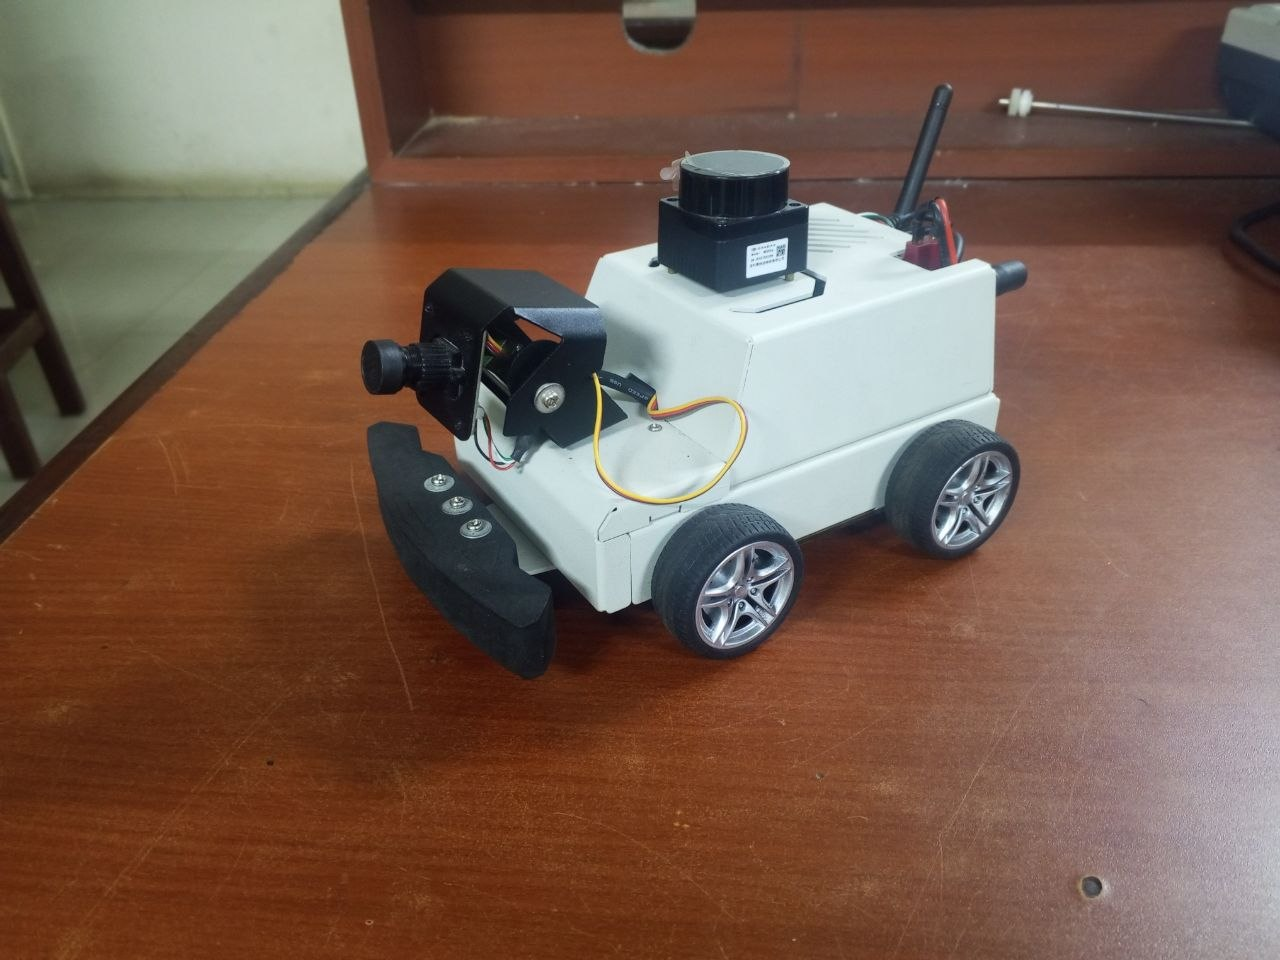
\includegraphics[width=0.68\textwidth]{assembled_robot_real.jpg}
\caption{Fully Assembled Yahboom MicroROS-Pi5 Autonomous Mobile Robot Platform}
\label{fig:physical_robot}
\end{figure}

\subsubsection{Primary Embedded Edge Computer (Raspberry Pi 5)}
The robot's central processing engine is a Raspberry Pi 5 single-board computer equipped with 8GB of high-speed LPDDR4X SDRAM, illustrated in Figure~\ref{fig:raspberry_pi_5}. Powered by a Broadcom BCM2712 quad-core ARM Cortex-A76 processor operating at 2.4~GHz, this edge computer possesses sufficient floating-point throughput to execute heavy computer vision and machine learning models in real time without offloading computations to external servers. High-bandwidth USB 3.0 interfaces support uncompressed video frame acquisition, while onboard gigabit networking and high-speed Wi-Fi allow live spatial telemetry streaming to remote developer monitoring stations. As established during integration testing (detailed in Section~\ref{sec:ram_planning}), the 8GB memory configuration is strictly essential to support concurrent execution of laser SLAM mapping and artificial intelligence inference without triggering kernel-level out-of-memory aborts.

\begin{figure}[H]
\centering
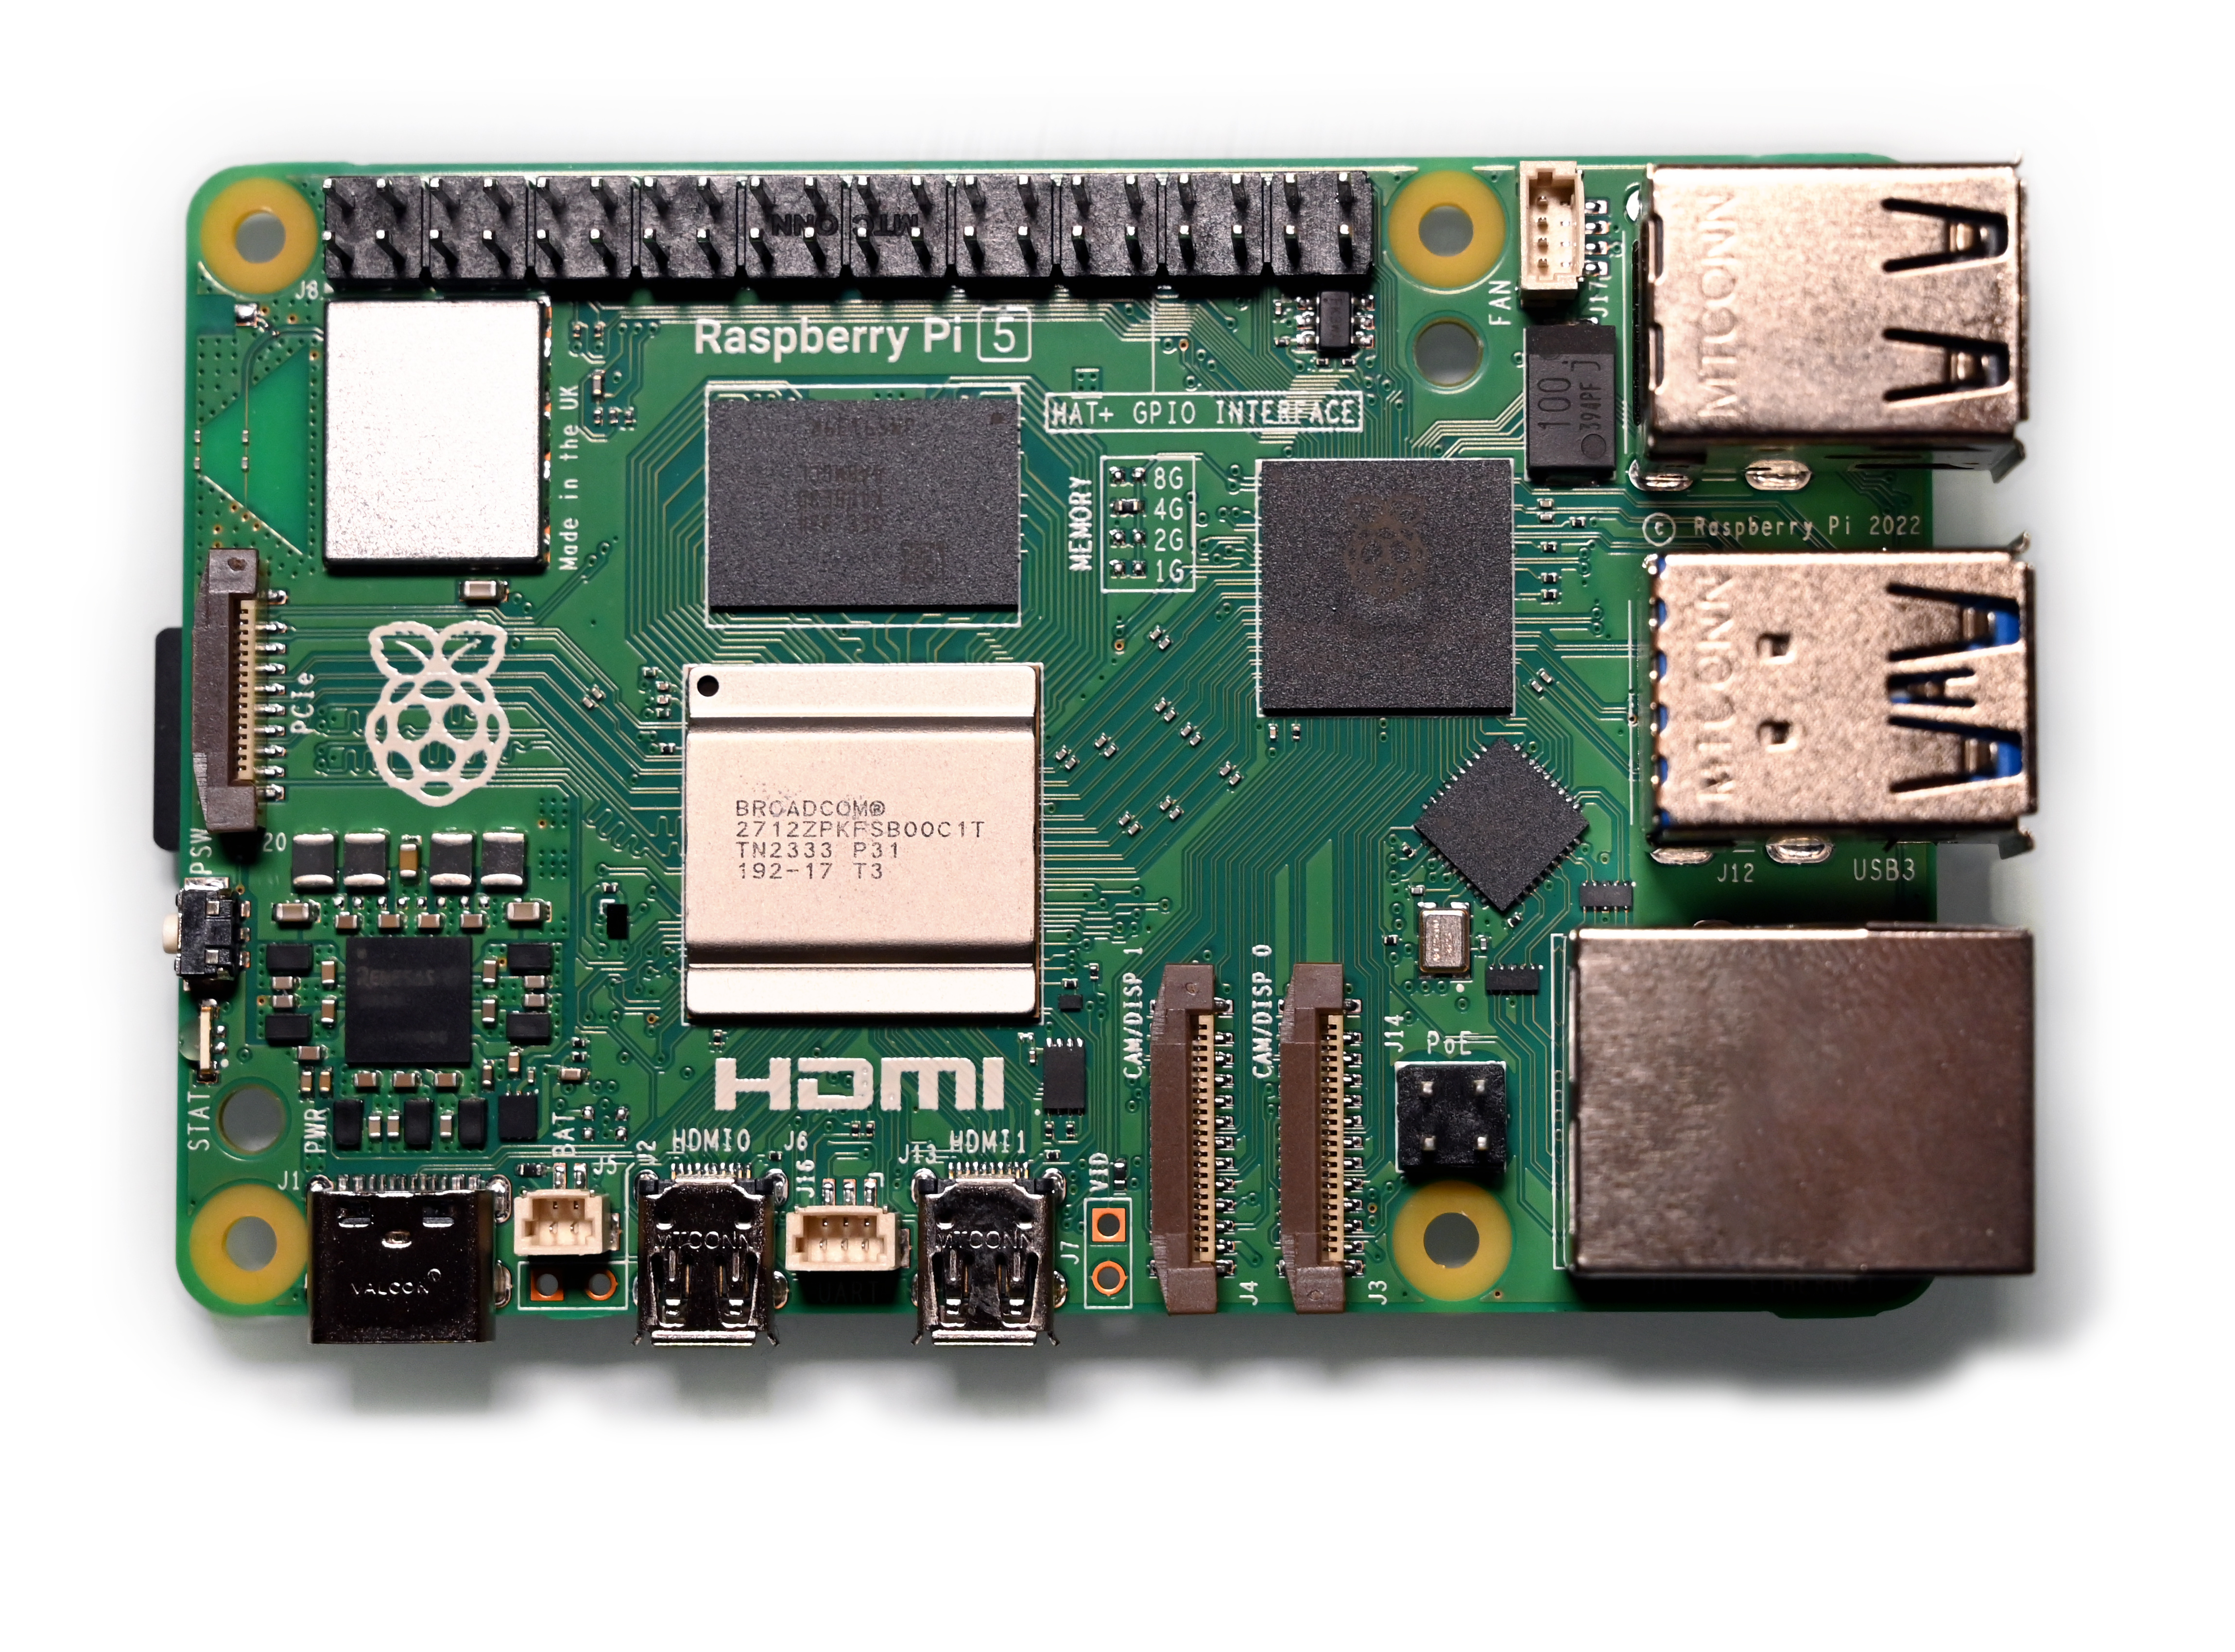
\includegraphics[width=0.68\textwidth]{raspberry_pi_5.jpg}
\caption{Raspberry Pi 5 Single-Board Computer (8GB LPDDR4X Edge Compute Node)}
\label{fig:raspberry_pi_5}
\end{figure}

\subsubsection{Embedded Microcontroller Co-Processor (MicroROS Expansion Board)}
Real-time actuator driving and deterministic sensor sampling are offloaded to a dedicated Yahboom MicroROS robot expansion board, illustrated in Figure~\ref{fig:microros_board}. The board is powered by an Espressif ESP32-S3 dual-core microcontroller running manufacturer FreeRTOS firmware configured as a micro-ROS client. The board integrates an onboard 4-channel H-bridge motor driver capable of delivering continuous high-current Pulse Width Modulation (PWM) signals to the DC drive motors. Additionally, it features a 6-axis MPU6050 Inertial Measurement Unit (IMU) that continuously registers 3-axis angular velocities and 3-axis linear accelerations. By communicating with the Raspberry Pi 5 over a dedicated UART serial connection at 921,600 baud, the expansion board acts as an immutable hardware bridge that isolates real-time motor control loops from high-level vision computing spikes.

\begin{figure}[H]
\centering
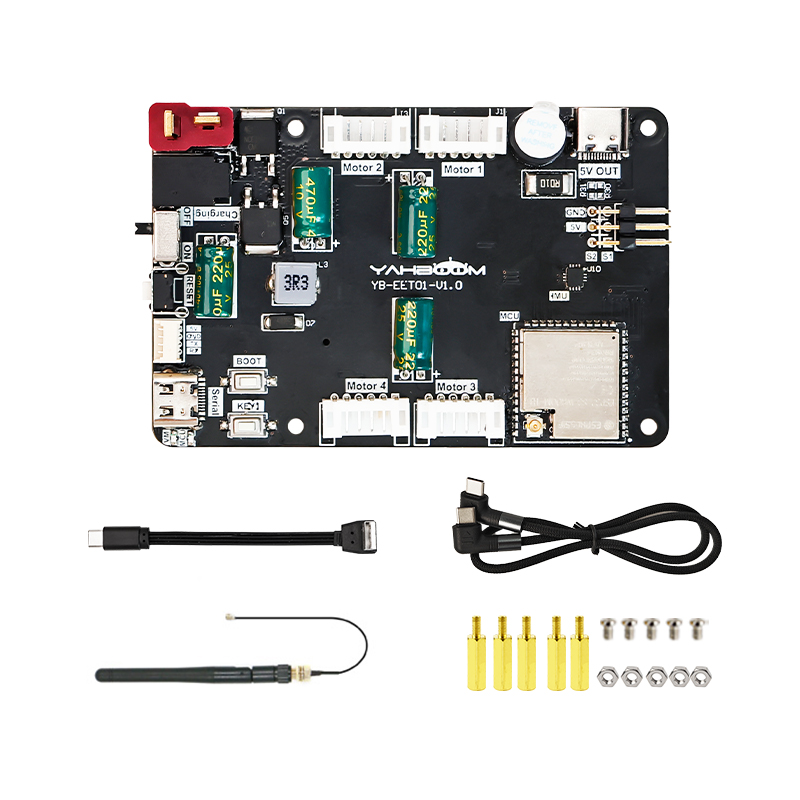
\includegraphics[width=0.68\textwidth]{microros_control_board.jpg}
\caption{Yahboom MicroROS Robot Expansion Board (ESP32-S3 Co-Processor)}
\label{fig:microros_board}
\end{figure}

\subsubsection{Planar Range Sensing (MS200 2D Time-of-Flight LiDAR)}
Environmental spatial awareness and collision safety are provided by an MS200 Time-of-Flight (ToF) 2D planar LiDAR sensor, shown in Figure~\ref{fig:ms200_lidar}. Mounted centrally on top of the robot's upper deck, the LiDAR continuously sweeps a 360-degree horizontal plane at a scan frequency of 12.5~Hz, emitting infrared laser pulses to measure object distances up to a 12-meter radius with millimeter resolution. Unlike traditional triangulation-based optical sensors, the ToF ranging principle provides superior immunity to ambient indoor illumination (up to 30~Klux), ensuring dependable obstacle detection under both bright fluorescent lighting and natural sunlight. In the software architecture, the LiDAR distance array feeds directly into the SLAM Toolbox occupancy mapping pipeline and enforces a hard-coded 0.36~m reactive collision stop.

\begin{figure}[H]
\centering
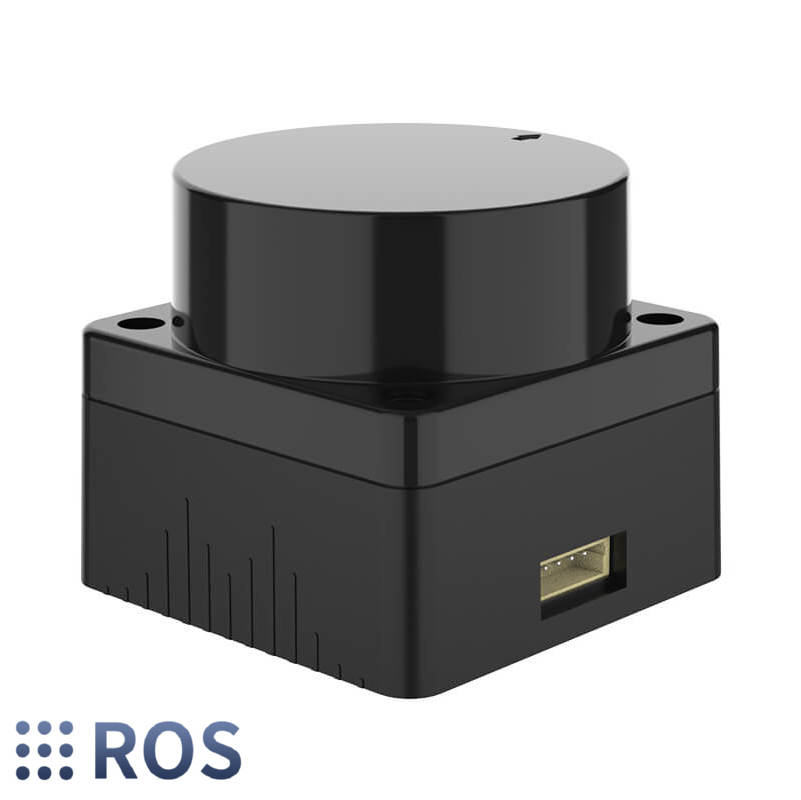
\includegraphics[width=0.55\textwidth]{ms200_lidar.jpg}
\caption{MS200 Time-of-Flight (ToF) 2D Planar LiDAR Sensor}
\label{fig:ms200_lidar}
\end{figure}

\subsubsection{Visual Perception and Active Camera Gimbal}
Visual data for human intention recognition is captured using an onboard 2MP USB monocular camera mounted upon a two-degree-of-freedom (2-DOF) pan-tilt servo gimbal mechanism, illustrated in Figure~\ref{fig:camera_gimbal}. The camera features a wide-angle optical lens configured to stream continuous RGB video at 20 frames per second with a resolution of $640 \times 480$ pixels. The active gimbal is actuated by two independent digital micro-servos (horizontal pan S1 and vertical tilt S2), enabling the camera to dynamically adjust its viewing orientation. When the robot enters person-tracking or visual-servoing modes, proportional control loops drive the gimbal servos to keep the interacting operator centered within the camera frame, maintaining uninterrupted skeletal hand tracking even as the robot turns or traverses uneven flooring.

\begin{figure}[H]
\centering
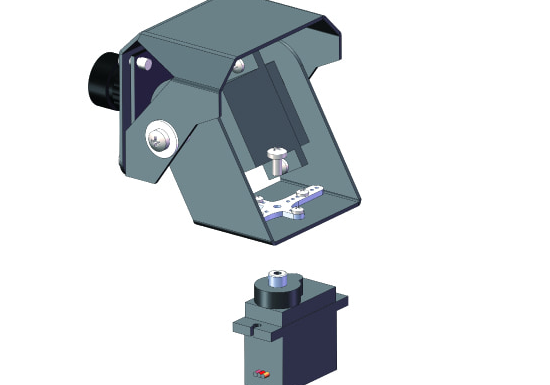
\includegraphics[width=0.55\textwidth]{camera_gimbal.png}
\caption{2-DOF Active Pan-Tilt Camera Gimbal Mechanism}
\label{fig:camera_gimbal}
\end{figure}

\subsubsection{Power Distribution, Battery Coupling, and Dual-Bus Regulation}
The mobile robot is energized by a 7.4V (nominal) 2000mAh 2-cell (2S) rechargeable lithium-ion battery pack mounted securely within the lower chassis. The battery wiring harness terminates in a keyed male plug that connects directly into the matching female DC power socket soldered onto the Yahboom MicroROS expansion board. When fully charged using the dedicated external balance charger, empirical voltage measurements taken across the terminal pins of this board-mounted female connector register above 7.0~V (typically ranging between 7.4~V and 8.2~V, up to an 8.4~V peak open-circuit potential). This direct DC rail supplies the high current demanded by the four DC wheel drive motors during rapid accelerations and continuous locomotion.

Because high-torque DC drive motors draw sharp transient current spikes during rapid acceleration and braking, directly sharing an unregulated power rail with sensitive computing electronics would cause severe voltage brownouts and processor resets. To ensure uninterrupted computation, the power subsystem implements a decoupled dual-bus architecture. While raw battery power feeds directly into the expansion board's H-bridge motor drivers, an integrated high-efficiency step-down buck converter regulates a clean, isolated 5V/5A power rail dedicated exclusively to powering the Raspberry Pi 5 single-board computer and its digital sensors. In this mechatronic topology, the Raspberry Pi 5 functions as the central Edge Computing Hub, orchestrating high-level visual cognition, multi-node ROS2 communication, and spatial mapping while remaining electrically insulated from motor-induced inductive noise.

Figure~\ref{fig:internal_wiring} depicts the physical mechatronic layout and wiring harness of the robot undergoing validation on the laboratory test bench prior to top casing installation. The stacked embedded computing architecture is clearly demonstrated, featuring the Raspberry Pi 5 mounted directly above the Yahboom MicroROS expansion board to minimize interconnect cable lengths. The dedicated wiring harness separates high-current motor power cables from low-voltage logic signal lines, while multi-conductor ribbon cables route quadrature encoder feedback and servo PWM lines directly into the ESP32-S3 microcontroller co-processor.

\begin{figure}[H]
\centering
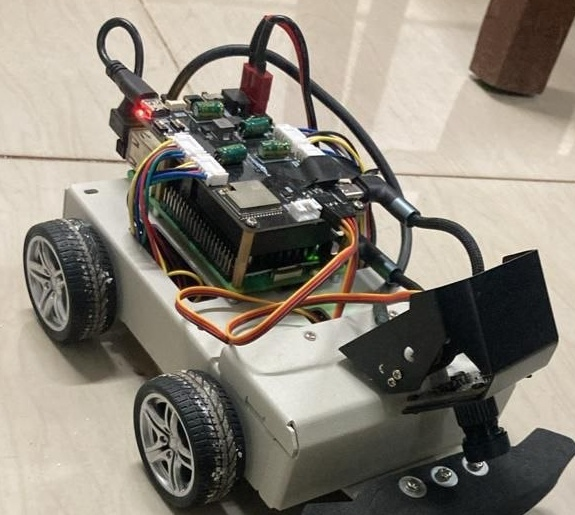
\includegraphics[width=0.55\textwidth]{robot_chassis_wiring.jpg}
\caption{Internal Chassis Hardware Integration and Mechatronic Wiring Harness (Uncased View)}
\label{fig:internal_wiring}
\end{figure}

\subsubsection{Consolidated Hardware Requirements Summary}
Table~\ref{tab:hardware_requirements} consolidates the technical specifications, physical parameters, and operational roles of all hardware components detailed in the preceding subsections. By establishing explicit performance thresholds for compute power, sensor range, and communication interfaces, this hardware baseline guarantees deterministic execution of both edge neural networks and real-time motor control loops. The complete Bill of Materials (BOM) integrates standard industrial-grade robotics modules, balancing high operational reliability against edge power consumption constraints.

\begin{table}[H]
\centering
\caption{Hardware Components, Technical Specifications, and Functional Roles}
\label{tab:hardware_requirements}
\renewcommand{\arraystretch}{1.15}
\begin{tabular}{|p{3.2cm}|p{4.8cm}|p{6.2cm}|}
\hline
\textbf{Component} & \textbf{Technical Specification} & \textbf{Project Functionality \& Operational Role} \\
\hline
Primary Computing Unit & Raspberry Pi 5, 8GB LPDDR4X SDRAM, quad-core ARM Cortex-A76 @ 2.4 GHz & Executes high-level perception pipeline (YOLOv8n spatial filter, MediaPipe hand tracker, MLP classifier, LSTM path predictor) and hosts Docker containers. \\
\hline
Robot Expansion Board & Custom ESP32-S3 co-processor; 4-channel motor driver; 2-channel servo PWM; 6-axis MPU6050 IMU & Operates micro-ROS client firmware; converts ROS2 velocity commands into motor PWM signals; streams encoder ticks and IMU angular velocity at 921,600 baud. \\
\hline
Mobile Chassis \& Locomotion & Yahboom industrial aluminium-alloy differential-drive platform; 4$\times$ 310 DC geared motors & Provides physical mobile locomotion; executes linear and angular motion trajectories; transmits quadrature wheel encoder feedback for dead-reckoning odometry. \\
\hline
Planar LiDAR Sensor & MS200 Time-of-Flight (ToF) 2D LiDAR; 12.5~Hz scan rate; 12~m range; 360$^\circ$ field of view & Delivers 2D laser range scans to \texttt{/scan} topic for SLAM Toolbox occupancy grid mapping; provides distance triggers for the 0.36~m reactive collision halt. \\
\hline
Monocular Vision Sensor & 2MP USB monocular CMOS camera (1080p @ 30 FPS, operated at 640$\times$480 @ 20 FPS) & Captures continuous frontal RGB video stream for person detection, spatial acceptance zone gating, hand cropping, and visual servoing tracking. \\
\hline
Active Camera Gimbal & 2-DOF pan-tilt servo mechanism with anti-windup angle clamping & Continuously tracks the operator's centroid; centers the human subject in the camera frame to maintain reliable visual gesture tracking during robot turns. \\
\hline
Power Supply \& Regulation & 7.4V 2000mAh rechargeable Li-ion battery pack with 5V/5A step-down buck converter & Supplies dual decoupled power rails: a regulated 5V rail for Raspberry Pi 5 logic and a direct rail for motor driver surges, preventing voltage drops and brownouts. \\
\hline
\end{tabular}
\end{table}

\subsection{Software Requirements}
\label{sec:software_requirements}
Table~\ref{tab:software_requirements} itemizes the software stack, operating systems, and robotics frameworks utilized across the development and physical deployment phases. In robotics engineering, software is typically divided between the ``developer workstation'' where intensive graphics, simulations, and code development take place, and the ``mobile robot'' where lightweight, battery-efficient programs execute in real time. This separation ensures that heavy visualization tasks—such as viewing live 3D laser maps—do not drain the robot's onboard processor or interfere with its physical movement decisions.

\begin{table}[H]
\centering
\caption{Software Components, Deployment Targets, and System Roles}
\label{tab:software_requirements}
\renewcommand{\arraystretch}{1.15}
\begin{tabular}{|p{3.8cm}|p{3.8cm}|p{6.6cm}|}
\hline
\textbf{Component} & \textbf{Deployment Target} & \textbf{System Role} \\
\hline
Ubuntu 24.04 LTS & Development Workstation & Host operating system for code development, neural network training, and simulation. \\
\hline
ROS2 Jazzy Jalisco & Development Workstation & Development middleware used for 3D spatial visualization (RViz2) and simulated testing. \\
\hline
Ubuntu 20.04 LTS & Robot (Docker Container) & Containerized Linux base environment hosting ROS2 Humble and hardware driver stacks. \\
\hline
ROS2 Humble Hawksbill & Robot (Docker Container) & Deployed robotics middleware providing reliable inter-process messaging via DDS transport. \\
\hline
Docker Engine 26.1 & Robot (Raspberry Pi 5) & Virtualization engine providing isolated, reproducible software containers on the mobile host. \\
\hline
MediaPipe HandLandmarker & Robot (\texttt{yahboom\_gesture}) & Vision model that tracks 21 anatomical landmarks on the human hand in real time. \\
\hline
Ultralytics YOLOv8n & Robot (\texttt{yahboom\_gesture}) & Lightweight neural network for detecting human bodies and filtering out background bystanders. \\
\hline
ONNX Runtime 1.18 & Robot (\texttt{yahboom\_gesture}) & High-performance cross-platform engine executing gesture classifier and trajectory models. \\
\hline
scikit-learn (joblib) & Robot (\texttt{yahboom\_gesture}) & Machine learning utility library for feature transformation and decoding model prediction labels. \\
\hline
SLAM Toolbox & Robot (\texttt{yahboom\_base}) & Laser-based mapping software that generates 2D indoor floor plans as the robot drives. \\
\hline
Navigation2 (Nav2) & Robot (\texttt{yahboom\_gesture}) & Autonomous navigation suite for waypoint path planning and obstacle-avoidance costmaps. \\
\hline
micro-ROS Client & ESP32-S3 Microcontroller & Real-time embedded firmware running on FreeRTOS; directly regulates motor PWM and sensors. \\
\hline
Python 3.10 / 3.12 & Both Targets & Primary programming language used to build all custom visual cognition and control nodes. \\
\hline
\end{tabular}
\end{table}

This architectural split reflects the resource-planning strategy detailed in Section~\ref{sec:ram_planning}. Development convenience on the workstation is cleanly decoupled from the strict execution requirements of the physically deployed robot, with containerization providing an immutable software boundary. The remote workstation allows human supervisors to observe the robot's camera feed and spatial maps comfortably over a wireless network without stealing memory or computational power from the robot itself.

\section{System Architecture Overview}
The system architecture of the autonomous mobile robot is structured around a multi-tiered hierarchy that clearly separates high-level cognitive perception from low-level physical actuation. In intuitive terms, this mirrors biological motor control: a central brain processes visual sights and formulates intentions, while a dedicated spinal reflex system translates those intentions into smooth physical muscle movements. By separating high-level neural inference from real-time motor pulse generation, each processor operates within its optimal performance limits without compromising mechanical responsiveness or physical safety.

Figure~\ref{fig:system_architecture} illustrates the overarching end-to-end system architecture and cognitive signal flow across the four primary operational tiers of the robot. Moving beyond isolated software components, this unified pipeline establishes deterministic intention-to-action coupling on edge hardware. Progressing sequentially from environmental sensing to mechanical wheel actuation, the pipeline coordinates sensory acquisition, spatial filtering, feature extraction, and motion arbitration across the embedded compute modules:
\begin{enumerate}
    \item \textbf{Tier 1: Multi-Modal Environmental Sensing:} The sensory layer captures simultaneous visual and range data from the surroundings. The monocular USB camera captures wide-angle frontal imagery at a resolution of $640 \times 480$ pixels operating at 20 frames per second (FPS), while the MS200 Time-of-Flight (ToF) LiDAR continuously sweeps a 360-degree horizontal plane at 12.5~Hz measuring distances from 0.12~m up to 12.0~m. Simultaneously, the onboard 6-axis IMU continuously samples chassis angular rates to support dead-reckoning odometry.
    \item \textbf{Tier 2: Spatial Perception and Operator Gating:} The perception layer filters the incoming video stream using a YOLOv8n spatial bounding box detector to isolate valid human bodies. Rather than processing the entire visual scene indiscriminately, a central spatial acceptance zone (spanning 45\% of the frame width and 65\% of the frame height) isolates the intended operator, rejecting peripheral bystanders. This stage computes the horizontal tracking error ($e_x = C_x - 320$) relative to the camera frame center to guide continuous visual servoing.
    \item \textbf{Tier 3: Feature Extraction and Gesture Classification:} For the isolated operator, MediaPipe HandLandmarker extracts 21 skeletal landmarks in real time. These coordinates are mathematically converted into a compact 19-dimensional scale-invariant geometric feature vector that is evaluated by a trained Multilayer Perceptron (MLP) running on the ONNX Runtime engine, completing inference in under 2~milliseconds.
    \item \textbf{Tier 4: Supervisory Control and Actuation:} The cognitive decision-making node (\texttt{brain\_node}) maintains a rolling consensus buffer and supervisory state machine to arbitrate driving commands. Validated velocity vectors (\texttt{/cmd\_vel}) are transmitted across the micro-ROS serial bridge at 921,600 baud to the ESP32-S3 co-processor, which directly generates motor PWM signals.
\end{enumerate}

In addition to this four-tier sequential cognition pipeline, Figure~\ref{fig:system_architecture} highlights an essential hard-wired safety mechanism: the planar LiDAR reactive safety bypass. If the MS200 LiDAR detects any physical obstacle within a critical 0.36~m protective safety bubble directly in front of the vehicle, the safety controller immediately overrides all active gesture commands and commands a zero-velocity halt. This reactive interlock line operates independently of visual perception and machine learning inference delays, ensuring guaranteed collision prevention in compliance with collaborative robot safety principles.

\begin{figure}[H]
\centering
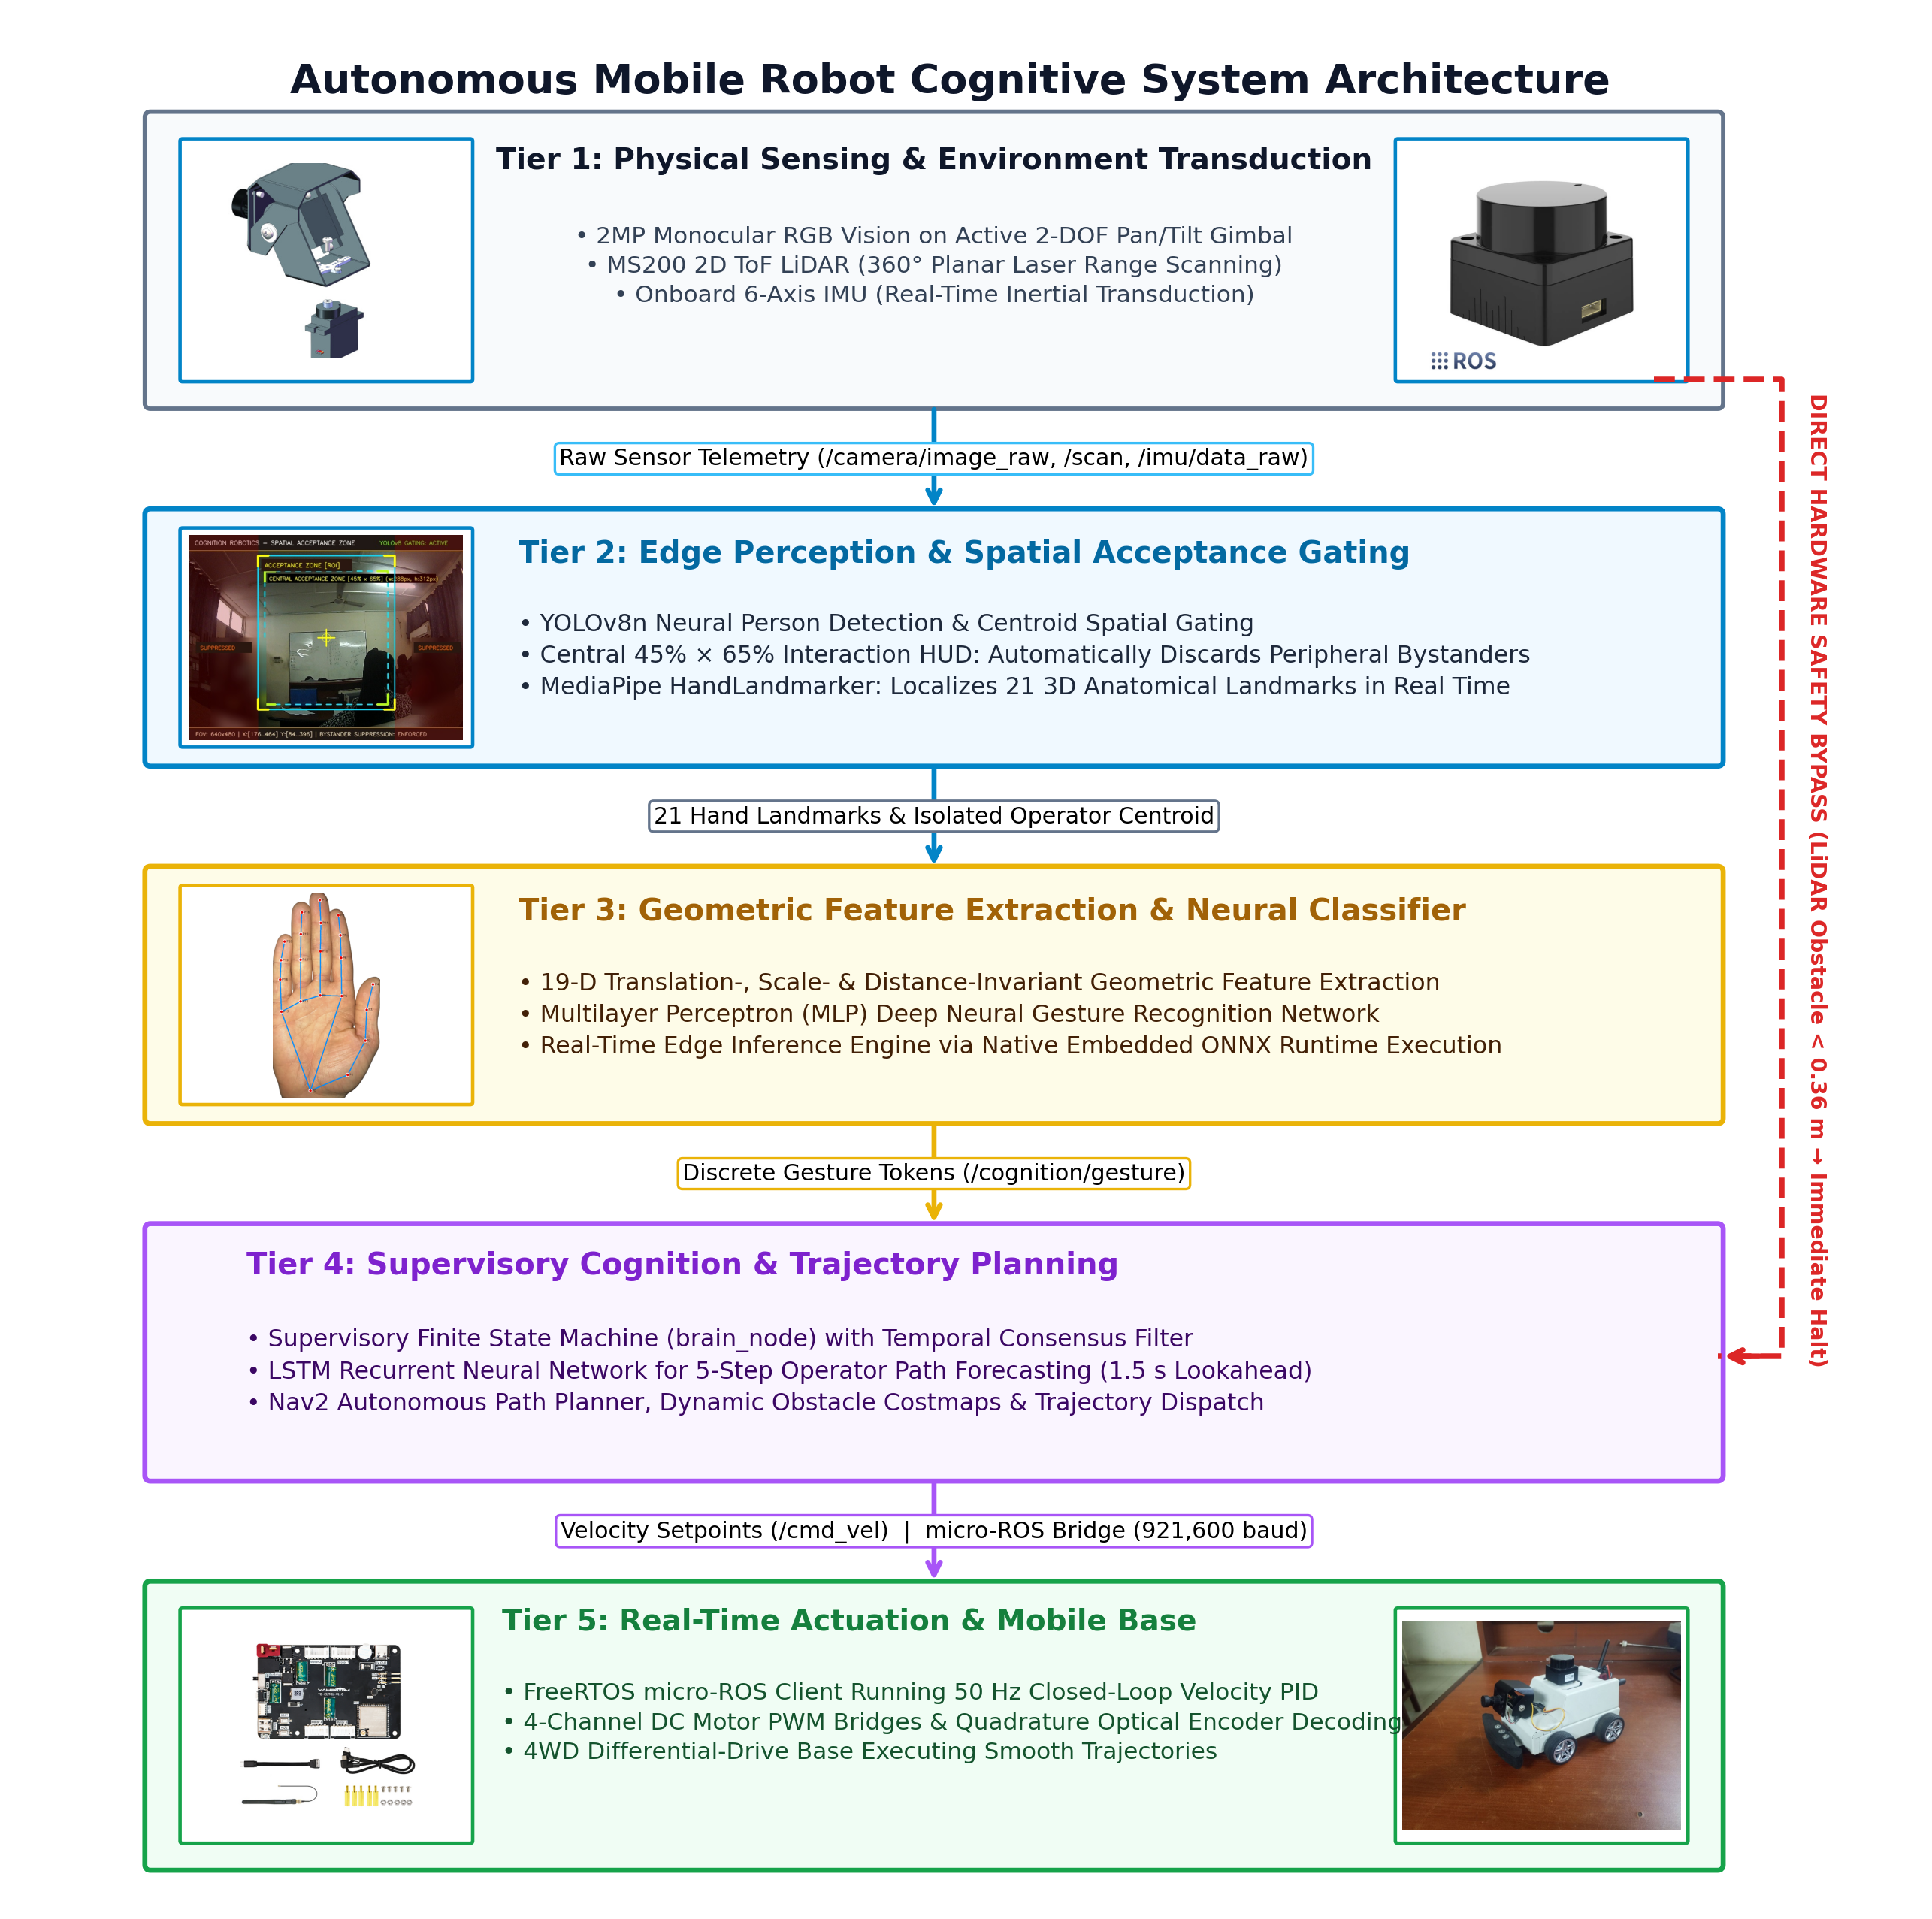
\includegraphics[width=0.88\textwidth]{system_architecture.png}
\caption{End-to-End System Architecture and Cognitive Signal Flow}
\label{fig:system_architecture}
\end{figure}

\subsection{Hardware Platform Specification}
The physical foundation of the system is the Yahboom MicroROS-Pi5 differential-drive mobile platform, an industrial aluminium-alloy robotic base designed for edge intelligence research. To achieve complete autonomy without relying on remote cloud servers or high-latency internet connections, the primary computing engine is a Raspberry Pi 5 single-board computer. This onboard computer functions as the primary edge computing node, executing vision models, neural network classifiers, and spatial navigation software entirely on edge hardware.

Low-level hardware management, power distribution, and motor driving are handled by a custom robotics expansion board powered by an ESP32-S3 microcontroller. This co-processor executes deterministic real-time motor commutation and low-level sensor sampling, interfacing directly with the four DC wheel motors, reading high-speed wheel rotation sensors (quadrature encoders), and polling an onboard 6-axis Inertial Measurement Unit (IMU). By offloading these time-sensitive hardware tasks to the ESP32-S3, the robot maintains steady wheel balance and responsive steering even when the main processor is busy running heavy vision algorithms.

For environmental awareness, the system utilizes an MS200 2D Time-of-Flight (ToF) LiDAR sensor mounted centrally on top of the chassis, emitting laser pulses to measure distances in a 360-degree flat circle 12.5 times per second. Visual perception for human interaction is provided by a 2MP monocular USB camera mounted on an active two-axis (pan-tilt) servo gimbal. This motorized gimbal provides two degrees of rotational freedom to maintain optical alignment with an interacting human operator, panning horizontally and tilting vertically to keep the human subject centered within the focal frame. Figure~\ref{fig:hardware_connection} illustrates the physical hardware interconnection and power distribution topology.

\begin{figure}[H]                                                                                                                                                                                                                                                                                                                                                                                                                                                                                                                                                                                                                                                                                                                                                                                                                                                                                                                                                                                                                                                                                                                                                                                                                                                                                                                                                                                                                                                                                                                                                                                                                                                                                                                                                                                                                                                                                                                                                                                                                                                                                                                                                                                                                                                                                                                                                                                                                                                                                                                                                                                                                                                                                                                                                                                                                                                                                                                                                                                                                                                                                                                                                                                                                                                                                                                                                                                                                                                                                                                                                                                                                                                                                                                                                                                                                                                                                                                                                                                                                                                                                                                                                                                                                                                                                                                                                                                                                                                                                                                                                                                                                                                                                                                                                                                                                                                                                                                                                                                                                                                                                                                                                                                                                                                                                                                                                                                                                                                                                                                                                                                                                                                                                                                                                                                                                                                                                                                                                                                                                                                                                                                                                                                                                                                                                                                                                                                                                                                                                                                                                                                                                                                                                                                                                                                                                                                                                                                                                                                                                                                                                                                                                                                                                                                                                                                                                                                                                                                                                                                                                                                                                                                                                                                                                                                                                                                                                                                                                                                                                                                                                                                                                                                                                                                                                                                                                                                                                                                                                                                                                                                                                                                                                                                                                                                                                                                                                                                                                                                                                                                                                                                                                                                                                                                                                                                                                                                                                                                                                                                                                                                                                                                                                                                                                                                                                                                                                                                                                                                                                                                                                                                                                                                                                                                                                                                                                                                                                                                                                                                                                                                                                                                                                                                                                                                                                                                                                                                                                                                                                                                                                                                                                                                                                                                                                                                                                                                                                                                                                                                                                                                                                                                                                                                                                                                                                                                                                                                                                                                                                                                                                                                                                                                                                                                                                                                                                                                                                                                                                                                                                                                                                                                                                                                                                                                                                                                                                                                                                                                                                                                                                                                                                                                                                                                                                                                                                                                                                                                                                                                                                                                                                                                                                                                                                                                                                                                                                                                                                                                                                                                                                                                                                                                                                                                                                                                                                                                                                                                                                                                                                                                                                                                                                                                                                                                                                                                       
\centering
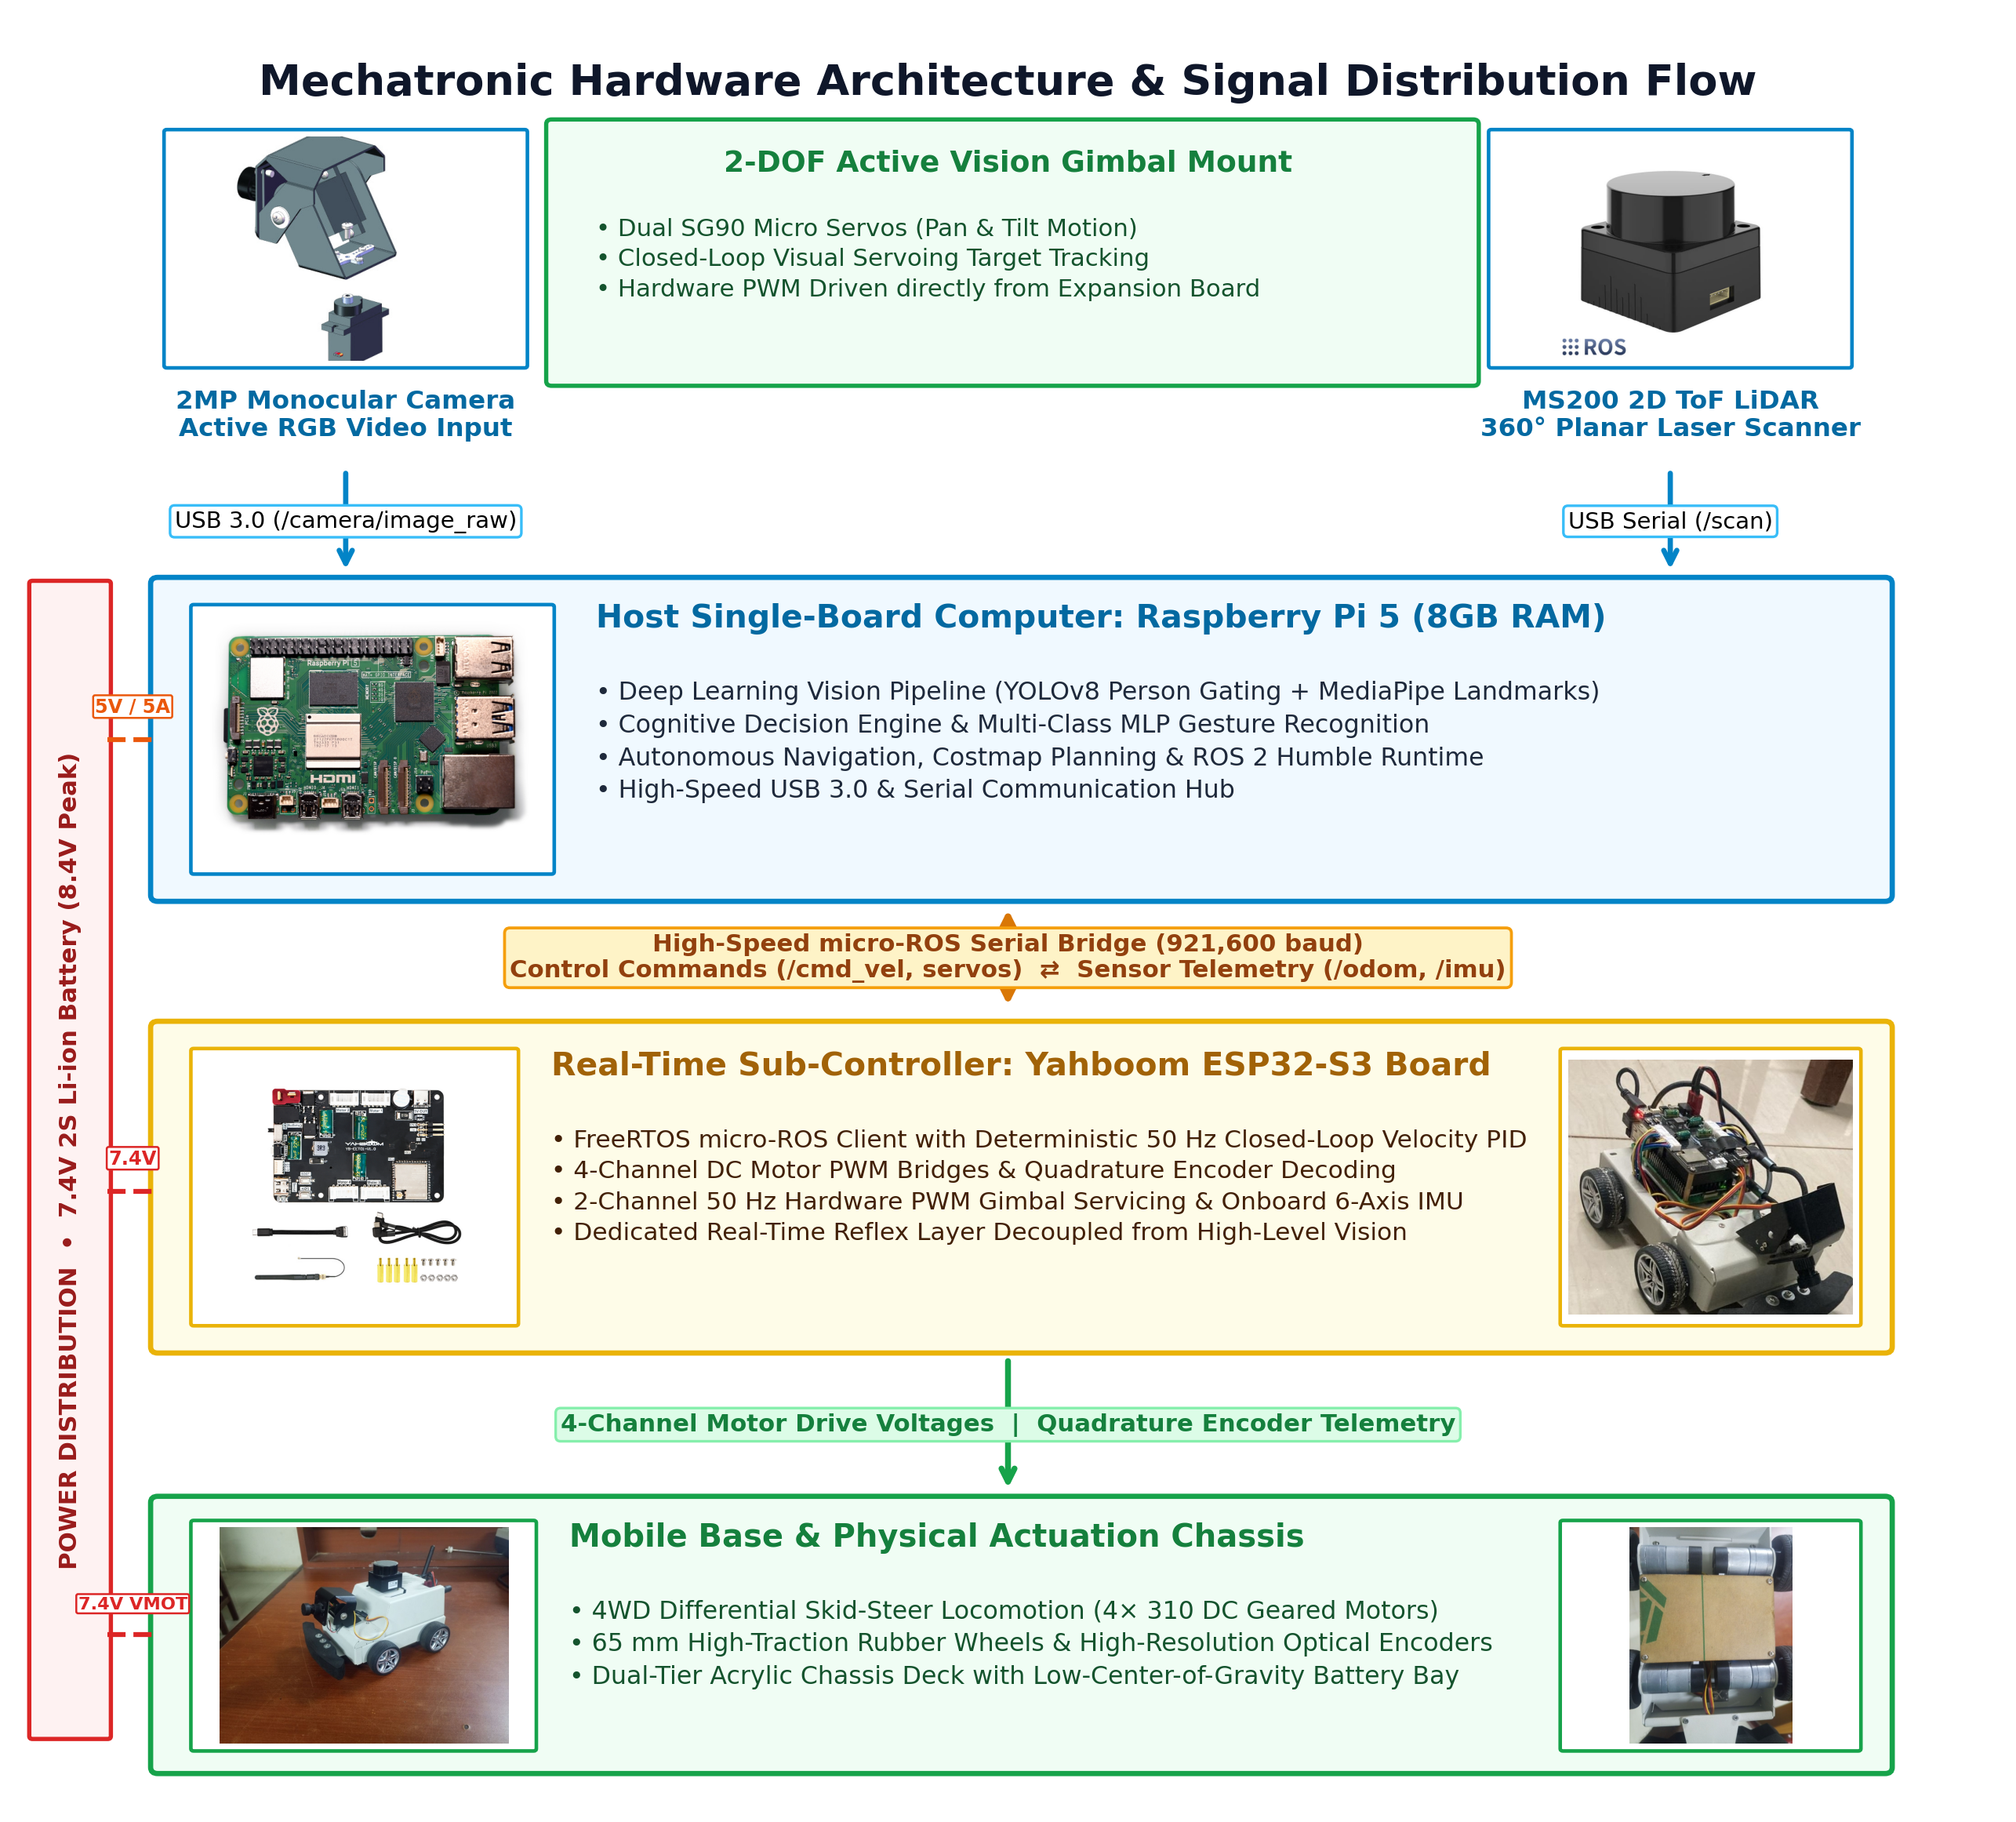
\includegraphics[width=0.88\textwidth]{hardware_design.png}
\caption{Hardware System Interconnection and Power Topology}
\label{fig:hardware_connection}
\end{figure}

\subsection{Software Framework and Deployment Strategy}
\label{sec:software_framework}
The software architecture is built natively on the Robot Operating System 2 (ROS2 Humble Hawksbill distribution) \cite{macenski2022}. ROS2 provides an asynchronous, distributed middleware framework enabling modular software nodes to exchange sensor telemetry and motion commands across standardized topic interfaces. To achieve optimal performance, high-level perception nodes are written in Python to leverage powerful machine learning libraries, whereas low-level motor drivers rely on the ESP32-S3's lightweight FreeRTOS real-time firmware.

Because small microcontrollers like the ESP32-S3 do not have enough memory to run a full Linux operating system, the board runs a specialized protocol called micro-ROS. This micro-ROS client communicates over a high-speed serial cable (operating at 921,600 baud) with a micro-ROS agent running on the Raspberry Pi, seamlessly integrating the microcontroller into the broader ROS2 network. This bridge allows the microcontroller to publish sensor data and receive driving instructions using standard ROS2 messages. By isolating time-critical motor control on the microcontroller, the robot prevents physical wheel stuttering if the main vision processor experiences a momentary computational spike.

To ensure software components run reliably without conflicting dependencies, all onboard software is organized into isolated virtual environments called Docker containers, enforcing strict process isolation and dependency encapsulation. This containerized strategy creates clean software boundaries, ensuring that third-party hardware drivers remain isolated from custom machine learning packages. The software architecture is partitioned across three distinct containers on the Raspberry Pi 5:
\begin{enumerate}
    \item \textbf{\texttt{yahboom\_base}}: Houses low-level hardware drivers, managing serial port communication, LiDAR scanning, and base chassis telemetry.
    \item \textbf{\texttt{micro\_ros\_agent}}: Serves as the real-time translation gateway between the ESP32-S3 microcontroller and the ROS2 messaging bus.
    \item \textbf{\texttt{yahboom\_gesture}}: Contains all custom cognition, computer vision, human detection, gesture classification, and decision-making nodes engineered in this study.
\end{enumerate}

All three containers are built upon Yahboom's official base image (\texttt{yahboomtechnology/ros-humble:4.1.2}), with the custom perception and control nodes layered cleanly on top within the \texttt{yahboom\_gesture} container. This layering strategy preserves tested factory hardware drivers while isolating newly developed artificial intelligence code in an easily modifiable user layer. As a result, experimental perception models can be revised and re-deployed in seconds without risking the stability of core chassis safety drivers.

All three containers are launched in Docker's \texttt{host} network mode, allowing them to share the host network stack directly rather than communicating through virtual network bridges. This direct communication allows ROS2's built-in discovery service to link nodes across container boundaries with sub-millisecond latency. Crucially, all containers and host drivers must share an identical communication domain setting known as the \texttt{ROS\_DOMAIN\_ID}. During early system integration, an elusive communication failure occurred when the micro-ROS hardware daemon and base driver container operated on domain 20, whereas custom perception nodes initialized on the default domain 0. This mismatch caused the robot to silently drop motor commands across the container boundary until all environments were standardized to \texttt{ROS\_DOMAIN\_ID=20}.

Finally, to make the robot fully self-sufficient upon battery power-up, all software containers are automatically initialized by an operating system background service (\texttt{cognition.service}). This ensures that the robot immediately begins listening for human gestures the moment the physical power switch is flipped, without requiring manual keyboard input. During testing, the robot operates headlessly without a monitor to conserve battery and memory, while developers monitor spatial maps and diagnostic cameras remotely over Wi-Fi using RViz2 on an \texttt{x86\_64} engineering host workstation (AMD Ryzen 5, 8GB DDR4 RAM running Ubuntu 24.04 LTS and ROS2 Jazzy Jalisco). Figure~\ref{fig:docker_deployment} illustrates this containerized multi-node deployment architecture.

\begin{figure}[H]
\centering
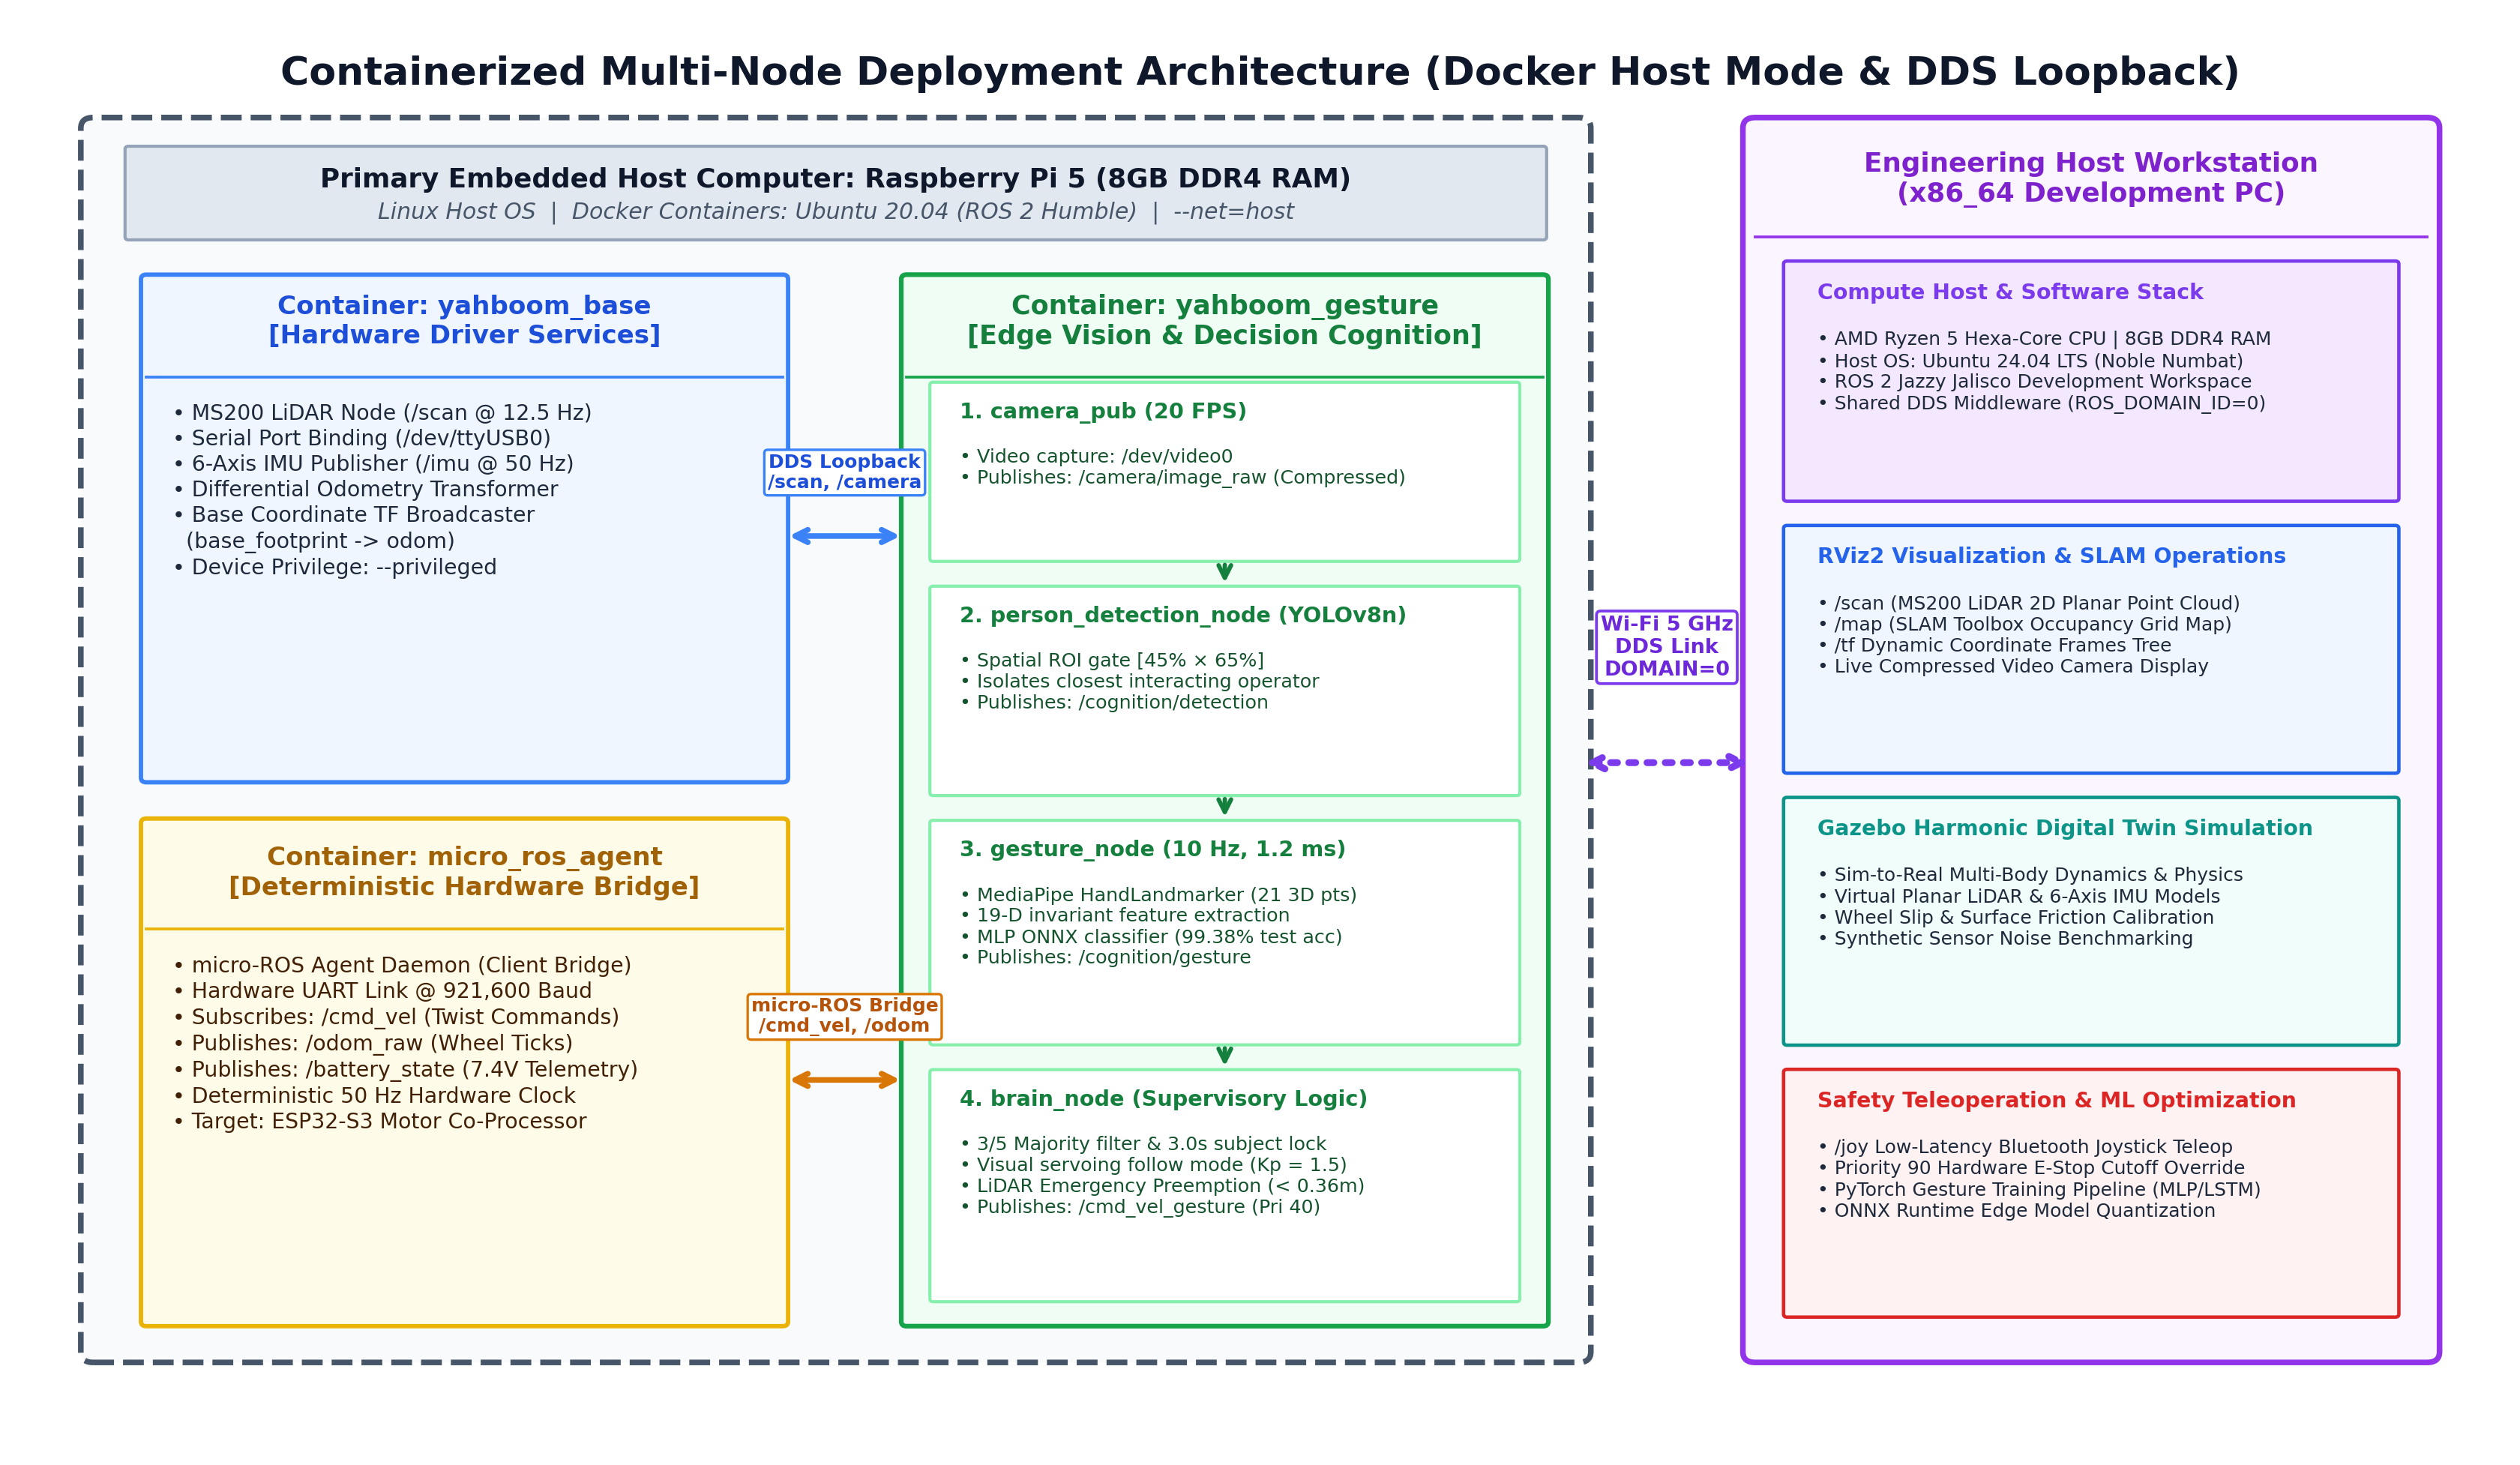
\includegraphics[width=0.88\textwidth]{fig_docker_deployment.png}
\caption{Containerized Multi-Node Deployment Architecture (Docker Host Mode)}
\label{fig:docker_deployment}
\end{figure}

\subsection{Hardware Resource Planning and Memory Constraints}
\label{sec:ram_planning}
During initial system prototyping, the platform was evaluated using a Raspberry Pi 5 equipped with 2GB of RAM, based on the preliminary hypothesis that individual perception and motion nodes would operate within a modest memory footprint. However, concurrent execution of the SLAM Toolbox laser mapping node alongside the full perception pipeline—comprising YOLOv8n spatial filtering, MediaPipe HandLandmarker keypoint extraction, and MLP neural inference—frequently exhausted physical memory, resulting in \texttt{std::bad\_alloc} exceptions. Under this constrained 2GB ceiling, critical ROS2 communication queues and costmap buffers saturated available physical memory, causing abrupt cessations of the \texttt{/scan} and camera video topics midway through live trials.

Diagnostic investigation confirmed that these process failures were triggered by the Linux Out-Of-Memory (OOM) killer terminating memory-intensive nodes to protect kernel execution. When the occupancy grid mapping array and neural network runtimes executed concurrently, aggregate memory consumption exceeded the physical capacity of the 2GB board. The resulting kernel terminations caused sudden communication drops across the inter-process message bus.

To resolve this bottleneck permanently, the physical hardware was upgraded to an 8GB LPDDR4X Raspberry Pi 5 single-board computer. This hardware upgrade eliminated memory allocation failures entirely, providing sufficient capacity to execute 2D laser SLAM, deep neural network inference, supervisory state logic, and telemetry logging simultaneously with over 3.8~GB of unallocated physical memory headroom remaining. Documenting this memory constraint is vital for engineering reproducibility, as it established the operational resource baseline and justified the Quality-of-Service (QoS) message queue depths implemented across the communication graph.

\section{Data Acquisition and Dataset Preparation}
To ensure the Multilayer Perceptron (MLP) gesture classifier performed reliably during physical deployment, a custom dataset was engineered specifically for this study. Utilizing pre-existing public gesture datasets often introduces a severe domain shift error, where external image corpora captured via desktop webcams fail to represent the low-angle perspective, wide-angle lens distortion, and optical characteristics of the robot's physical mounting. In contrast, an autonomous mobile robot interacts from a low-elevation optical vantage point subject to varying indoor lighting and background activity. By acquiring all training samples directly through the robot's onboard optical sensor, the neural network learned representations that accurately reflect the focal geometry, mounting height, and lens distortion encountered during live physical trials.

\subsection{Recording Conditions and Class Balancing}
\label{sec:recording_conditions}
The dataset was constructed to encompass the six explicit operational commands: STOP, GO, LEFT, RIGHT, BACK, and FOLLOW. To ensure the neural network learned the geometric relationships of the hand rather than memorizing the background, data collection was conducted across three distinct indoor environments with varying conditions of natural daylight and artificial fluorescent lighting. Operators were positioned at realistic operational distances ranging between 1.0~m and 2.5~m from the robot.

To prevent model bias toward any specific gesture, the dataset was strictly balanced. Exactly 1,000 distinct frames were recorded for each of the six gesture classes, resulting in a total dataset of 6,000 labeled instances. During recording, the operator performed micro-variations of each gesture (altering wrist roll, pitch, and yaw within a 15-degree tolerance) to ensure the model generalized effectively to natural, imperfect human inputs.

\subsection{Preprocessing and Train-Test Splitting}
The raw captured frames were not fed directly into the model. To mirror the live inference pipeline exactly, the raw dataset was processed through the YOLOv8n spatial filter to generate bounding boxes, followed by the MediaPipe HandLandmarker to extract the 21 anatomical coordinates. Quality assurance filtering automatically rejected frames where extreme motion blur or severe physical occlusion prevented MediaPipe from achieving minimum landmark tracking confidence ($\ge 0.50$), ensuring high signal integrity across the training set. The extracted coordinates were then mathematically converted into the 19 normalized geometric features.

Prior to training, the finalized 6,000-sample feature dataset was randomly shuffled and partitioned using a standard machine learning distribution ratio: 70\% (4,200 samples) allocated for training the model, 15\% (900 samples) reserved for continuous validation during training, and 15\% (900 samples) isolated as a blind test set to evaluate final classification accuracy. This strict partitioning ensured that the model's reported test performance was evaluated entirely on unseen samples. Isolating a distinct 15\% holdout partition ensured that model generalization was rigorously evaluated on unseen geometric feature distributions, guarding against empirical overfitting and confirming that the classifier learned robust decision boundaries across all operational gestures.

\subsection{Dataset Statistics}
This section provides a detailed tabular breakdown of the gesture dataset described in Section~\ref{sec:recording_conditions} and Section 3.4.2. Table~\ref{tab:class_distribution} presents the per-class distribution across the 6,000 recorded frames, while Table~\ref{tab:dataset_split} details the train, validation, and test partitions. Maintaining an identical quota of 1,000 samples for each command prevented artificial class bias, guaranteeing that the robot would not favor common gestures (such as STOP) over rotational steering commands (such as LEFT or RIGHT).

\begin{table}[H]
\centering
\caption{Per-Class Sample Distribution}
\label{tab:class_distribution}
\begin{tabular}{|l|c|c|}
\hline
\textbf{Gesture Class} & \textbf{Samples} & \textbf{Share of Dataset} \\
\hline
STOP & 1,000 & 16.7\% \\
\hline
FOLLOW & 1,000 & 16.7\% \\
\hline
GO & 1,000 & 16.7\% \\
\hline
LEFT & 1,000 & 16.7\% \\
\hline
RIGHT & 1,000 & 16.7\% \\
\hline
BACK & 1,000 & 16.7\% \\
\hline
\textbf{Total} & \textbf{6,000} & \textbf{100.0\%} \\
\hline
\end{tabular}
\end{table}

\begin{table}[H]
\centering
\caption{Train / Validation / Test Split}
\label{tab:dataset_split}
\begin{tabular}{|l|c|c|}
\hline
\textbf{Split} & \textbf{Samples} & \textbf{Proportion} \\
\hline
Training & 4,200 & 70.0\% \\
\hline
Validation & 900 & 15.0\% \\
\hline
Test & 900 & 15.0\% \\
\hline
\textbf{Total} & \textbf{6,000} & \textbf{100.0\%} \\
\hline
\end{tabular}
\end{table}

Data collection spanned three distinct indoor environments with varying natural and artificial fluorescent lighting conditions. Micro-variations in wrist roll, pitch, and yaw (within a 15-degree tolerance) were systematically introduced during recording to improve model robustness. This balanced structure provided a stable foundation for training the gesture classifier.

\section{Perception and Intention Recognition Pipeline}
The perception pipeline was designed as a sequential filter to isolate and classify human hand gestures from raw visual data. This architecture was specifically optimized for localized inference, allowing the system to extract precise features and execute classification models natively on the edge processor. The pipeline isolated a valid human operator, extracted anatomical hand landmarks, engineered scale-invariant geometric features, and classified the intended gesture.

\subsection{Spatial Zone Person Detection}
The first stage of the perception pipeline utilized the YOLOv8n (nano variant) object detection model \cite{yolov8_ultralytics} to detect human presence in the camera field of view. During initial development and empirical testing, a critical vulnerability was observed: the downstream skeletal tracking framework would unpredictably extract landmarks from any visible hand in the camera frame. In environments with multiple individuals, the robot would erroneously lock onto background movements or gestures performed by non-operators, leading to erratic system behavior.

To resolve this interference and enforce operational safety, a spatial zone filter was engineered over the raw YOLOv8n bounding box outputs. On the standard $640 \times 480$ pixel video frame, the camera's field of view was programmatically partitioned into a central active acceptance zone spanning 45\% of the frame width ($288\,\text{pixels}$) and 65\% of the frame height ($312\,\text{pixels}$). This defines an explicit horizontal acceptance window of $X \in [176, 464]$ and a vertical window of $Y \in [84, 396]$ centered at $(320, 240)$. For every detected human candidate, the system evaluates the 2D bounding box coordinates $[x_{\min}, y_{\min}, w, h]$ and calculates the horizontal and vertical centroid $(B_x, B_y)$ as defined in Equation~\eqref{eq:centroid}:
\begin{equation}
\label{eq:centroid}
B_x = x_{\min} + \frac{w}{2}, \quad B_y = y_{\min} + \frac{h}{2}
\end{equation}
Evaluating this spatial centroid ensures that the operator is actively facing the robot and centered within its immediate operational corridor before any downstream skeletal landmark extraction or gesture interpretation takes place. By referencing the candidate's center of mass against this predefined spatial boundary, spurious peripheral movements are ignored before consuming CPU cycles. This geometric constraint provides a robust first line of defense against false activations in busy collaborative workspaces.

Figure~\ref{fig:spatial_zone} illustrates this empirical spatial receptive zone perception and the accompanying ISO 5807 decision flowchart, contrasting the active operator targeting box against peripheral bystanders who are filtered out and protected by Gaussian privacy blurring. In accordance with the decision logic, a candidate detection is accepted as an operator only if its centroid satisfies $176 \le B_x \le 464$ and $84 \le B_y \le 396$. If multiple persons occupy the camera frame, the system evaluates up to three candidates, selecting the largest (closest) zone-eligible bounding box as the active operator. When an operator issues a gesture that passes the 5-frame consensus threshold described in Section~\ref{sec:temporal_buffering}, the \texttt{brain\_node} establishes a 3-second operational lock, during which background bystanders outside the central zone are rejected from interfering with the robot's navigation path.

\begin{figure}[H]
\centering
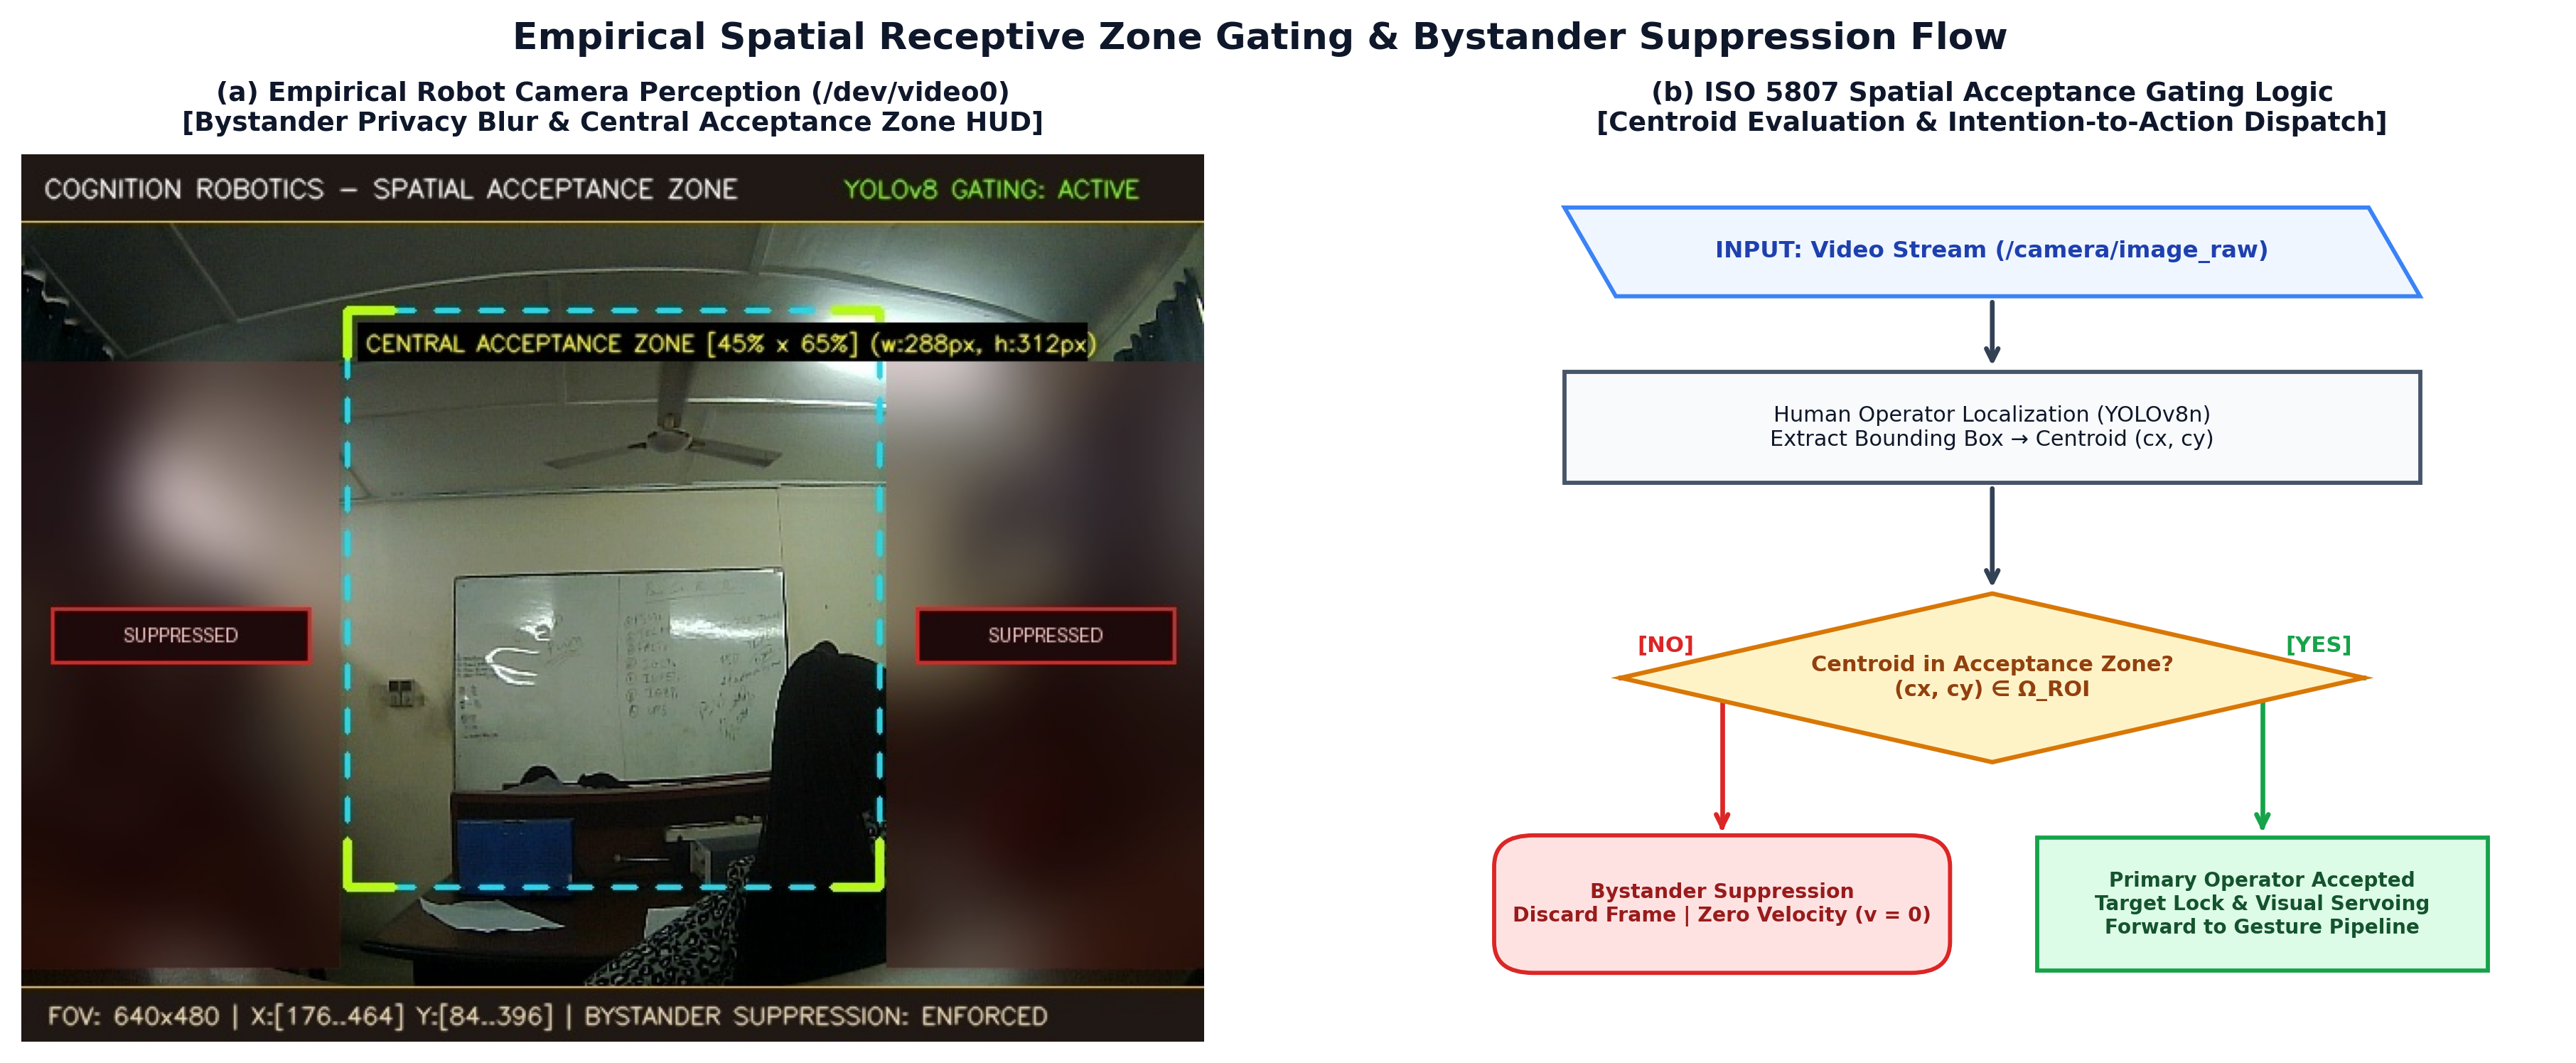
\includegraphics[width=0.88\textwidth]{fig_spatial_zone.png}
\caption{Empirical Spatial Receptive Zone Gating and Bystander Suppression Flow}
\label{fig:spatial_zone}
\end{figure}

This geometric spatial zone filter relies on horizontal bounding-box coordinates to isolate the primary operator, prioritizing low computational overhead during real-time interaction. In crowded environments where multiple individuals enter the central zone concurrently, spatial heuristic disambiguation defaults to selecting the candidate with the largest projected bounding box area. To evaluate unique individual identification, a biometric facial recognition pipeline was developed using InsightFace (buffalo\_sc MobileFaceNet generating 512-dimensional ArcFace embeddings). Offline verification confirmed clear separation between enrolled operators (cosine similarity 0.54--0.57) and unauthorized individuals (0.09). Because running concurrent deep face detection on the edge CPU would constrain gesture inference latency, continuous biometric authentication was preserved as a modular architecture targeted for dedicated onboard NPU acceleration in future iterations.

\subsection{Vision-Based Hand Tracking}
Once an operator was successfully isolated within the spatial zone, the pipeline engaged the MediaPipe HandLandmarker framework \cite{lugaresi2019mediapipe} for skeletal tracking. This framework extracted high-fidelity anatomical data from the 2D monocular camera feed. MediaPipe fits a 2.5D topological skeletal model to the localized hand region, outputting 21 distinct anatomical landmarks corresponding to the wrist, metacarpophalangeal, interphalangeal, and fingertip joints in real time.

For each valid frame containing the primary operator, the node identified the spatial coordinates of 21 specific hand landmarks, including the wrist, knuckles, and fingertips. Each landmark was output as a normalized three-dimensional coordinate $(x, y, z)$. While this provided a detailed topological representation of the hand, feeding these raw, unscaled coordinates directly into a lightweight classifier introduced significant statistical variance depending on the operator's physical distance from the camera. Consequently, these raw landmarks served strictly as the foundational input for the subsequent geometric feature engineering stage.

\subsection{Geometric Feature Engineering}
To ensure the classification model remained robust regardless of the operator's distance from the camera, the raw spatial landmarks were transformed into a set of scale-invariant geometric features. In computer vision, an object close to the lens appears large on screen, while the same object positioned several meters away appears tiny, even though its physical geometry has not changed. If a neural network attempts to classify gestures using raw pixel coordinates, it easily confuses changes in distance with changes in hand shape. To overcome this limitation, the raw anatomical coordinates were transformed into scale-invariant geometric features—calculating relative angles and normalized joint ratios that remain identical whether the operator stands one meter or three meters away from the robot.

The feature extraction pipeline executes three sequential mathematical operations: origin translation, scale normalization, and joint angle derivation. First, to ensure invariance against hand translation within the camera frame, the wrist landmark ($\mathbf{p}_0$) is designated as the local coordinate origin $(0,0,0)$. All twenty remaining hand landmark coordinates ($\mathbf{p}_i = [x_i, y_i, z_i]^T$) are translated relative to this origin as defined in Equation~\eqref{eq:wrist_translation}:
\begin{equation}
\label{eq:wrist_translation}
\mathbf{p}'_i = \mathbf{p}_i - \mathbf{p}_0, \quad \text{for } i \in \{0, 1, \dots, 20\}
\end{equation}
By referencing all twenty remaining anatomical keypoints directly to the wrist origin, the resulting coordinate structure becomes completely immune to the hand's absolute Cartesian position in the camera frame. In mathematical terms, this shifts the coordinate system from camera space to hand-centric space. Consequently, an operator holding their hand high in the frame produces an identical coordinate representation to one holding their hand low.

Second, to achieve scale invariance across varying operating distances, the translated coordinates are normalized by the operator's anatomical palm width ($W_{\text{palm}}$). In physical human anatomy, the distance across the knuckles remains constant regardless of the viewer's vantage point. The palm width is computed as the 3D Euclidean distance between the index metacarpophalangeal joint (Landmark 5) and the pinky metacarpophalangeal joint (Landmark 17) using Equation~\eqref{eq:palm_width}:
\begin{equation}
\label{eq:palm_width}
W_{\text{palm}} = \|\mathbf{p}'_5 - \mathbf{p}'_{17}\| = \sqrt{(x'_5 - x'_{17})^2 + (y'_5 - y'_{17})^2 + (z'_5 - z'_{17})^2}
\end{equation}
To scale each coordinate proportionally, each translated landmark and fingertip distance is subsequently divided by this reference palm width. This normalization ensures that visual features reflect true anatomical proportions rather than distance-dependent pixel sizes. The transformation is computed per Equation~\eqref{eq:scale_norm}:
\begin{equation}
\label{eq:scale_norm}
\hat{\mathbf{p}}_i = \frac{\mathbf{p}'_i}{W_{\text{palm}}}
\end{equation}
This proportional division guarantees that the resulting numerical values remain constant whether the user interacts near the camera lens or several meters away in the room. Even under significant forward-backward motion, the normalized coordinates maintain consistent numerical bounds. This eliminates the need to train separate distance-dependent gesture models.

Third, to determine whether individual fingers are curled or extended independently of hand tilt in space, the system derives 3D cosine joint curl angles. For each of the five digits, vector $\vec{u}$ represents the bone segment between the metacarpophalangeal (MCP) and proximal interphalangeal (PIP) joints, while vector $\vec{v}$ represents the segment between the PIP and fingertip (TIP) joints. The curl angle ($\theta_j$) is calculated using the vector dot product formulation in Equation~\eqref{eq:curl_angle}:
\begin{equation}
\label{eq:curl_angle}
\theta_j = \arccos\left(\frac{\vec{u} \cdot \vec{v}}{\|\vec{u}\| \|\vec{v}\|}\right)
\end{equation}
When a finger is extended straight outward, the angle $\theta_j$ approaches zero radians ($0^\circ$). As the finger curls tightly into the palm, the angle smoothly increases toward $\pi$ radians ($180^\circ$). As summarized in Table~\ref{tab:geometric_features}, combining these normalized fingertip distances, finger curl angles, inter-finger spread angles, and thumb spatial depth yields a compact, 19-dimensional feature vector.

\begin{table}[H]
\centering
\caption{Engineered Geometric Features (19 total)}
\label{tab:geometric_features}
\begin{tabular}{|c|l|l|}
\hline
\textbf{\#} & \textbf{Feature} & \textbf{Description} \\
\hline
1 & Thumb curl angle & Angle between MCP--PIP and PIP--TIP segments \\
\hline
2 & Index curl angle & Angle between MCP--PIP and PIP--TIP segments \\
\hline
3 & Middle curl angle & Angle between MCP--PIP and PIP--TIP segments \\
\hline
4 & Ring curl angle & Angle between MCP--PIP and PIP--TIP segments \\
\hline
5 & Pinky curl angle & Angle between MCP--PIP and PIP--TIP segments \\
\hline
6 & Thumb--Index spread & Angle between thumb and index tip vectors (from wrist) \\
\hline
7 & Index--Middle spread & Angle between index and middle tip vectors (from wrist) \\
\hline
8 & Middle--Ring spread & Angle between middle and ring tip vectors (from wrist) \\
\hline
9 & Thumb tip distance & Thumb tip--to--wrist distance, normalized by palm width \\
\hline
10 & Index tip distance & Index tip--to--wrist distance, normalized by palm width \\
\hline
11 & Middle tip distance & Middle tip--to--wrist distance, normalized by palm width \\
\hline
12 & Ring tip distance & Ring tip--to--wrist distance, normalized by palm width \\
\hline
13 & Pinky tip distance & Pinky tip--to--wrist distance, normalized by palm width \\
\hline
14 & Palm angle & Angle of middle-MCP--to--wrist vector vs. vertical reference \\
\hline
15 & Index pointing angle & 2D angle of the index finger's direction vector \\
\hline
16 & Thumb pointing angle & 2D angle of the thumb's direction vector \\
\hline
17 & Index--Thumb angle & Angle between index and thumb vectors (from wrist) \\
\hline
18 & Thumb--Index tip distance & Distance between thumb tip and index tip, normalized \\
\hline
19 & Thumb height & Thumb tip depth (z-axis) relative to wrist \\
\hline
\end{tabular}
\end{table}

\subsection{Gesture Classification Model}
\label{sec:gesture_classification_model}
An initial implementation of the gesture classification subsystem utilized a rule-based heuristic classifier, applying static geometric thresholds directly to the 19 engineered features. While functional for a small set of orthogonal hand configurations, this deterministic heuristic approach proved brittle during dynamic interaction. Small variations in hand orientation, distance from the camera, and natural inter-operator biomechanical differences frequently caused feature vectors to oscillate across hand-tuned boundaries, requiring continuous manual recalibration. This operational brittleness motivated the transition to a supervised Multilayer Perceptron (MLP) classifier, which learns continuous, non-linear decision boundaries across empirical data distributions, generalizing effectively across natural morphological variations in human gesture execution.

With the spatial data reduced to 19 scale-invariant features, the final stage of the perception pipeline was the classification of the intentional command using this MLP. The neural network was architected as a compact feedforward model consisting of four fully-connected layers: an input layer of 19 feature nodes, a primary hidden layer of 128 neurons, a secondary hidden layer of 64 neurons, and an output layer of 6 classification neurons ($19 \to 128 \to 64 \to 6$). The hidden layers incorporate Rectified Linear Unit (ReLU) activation functions ($\text{ReLU}(z) = \max(0, z)$) to capture complex non-linear combinations of finger flexions, while the final layer employs a Softmax activation function to generate normalized posterior probability distributions across the six discrete commands: STOP, GO, LEFT, RIGHT, BACK, and FOLLOW. By minimizing structural parameter depth, the forward inference pass executes in under 2~milliseconds on the Raspberry Pi 5 CPU via the ONNX Runtime engine.

The model development protocol comprised two iterative training cycles. An initial preliminary dataset of 3,000 samples yielded an initial test accuracy of 99.67\%; however, class representation was skewed toward static poses. To establish rigorous cross-class generalization and eliminate classification bias, the dataset was expanded to a fully balanced distribution of 6,000 samples (1,000 samples per class across six distinct commands). On this standardized holdout benchmark, the MLP classifier achieved a 99.38\% test accuracy, demonstrating uniform class sensitivity and robust geometric discrimination across all six operational commands.

The final trained classifier was exported to Open Neural Network Exchange (ONNX) format (\texttt{gesture\_model.onnx}) and loaded via ONNX Runtime (\texttt{onnxruntime.InferenceSession}) inside \texttt{gesture\_node} at runtime, with a separate \texttt{label\_encoder\_pi.pkl} file—loaded via scikit-learn's joblib—handling decoding of the model's integer output back to a gesture label string. ONNX Runtime was used consistently across both learned models in the perception pipeline, providing a uniform inference approach for the gesture classifier and the LSTM path predictor alike. The raw classification output was then published to the ROS2 middleware, where it was intercepted by the centralized decision-making node. Figure~\ref{fig:feature_pipeline} illustrates this complete four-stage pipeline: starting from the 21 MediaPipe anatomical hand landmarks extracted from empirical camera data ($P_0$ through $P_{20}$), progressing through scale and translation invariance transforms, constructing the 19-dimensional invariant geometric feature vector, and terminating in the low-latency Multilayer Perceptron classifier generating discrete action tokens.

\begin{figure}[H]
\centering
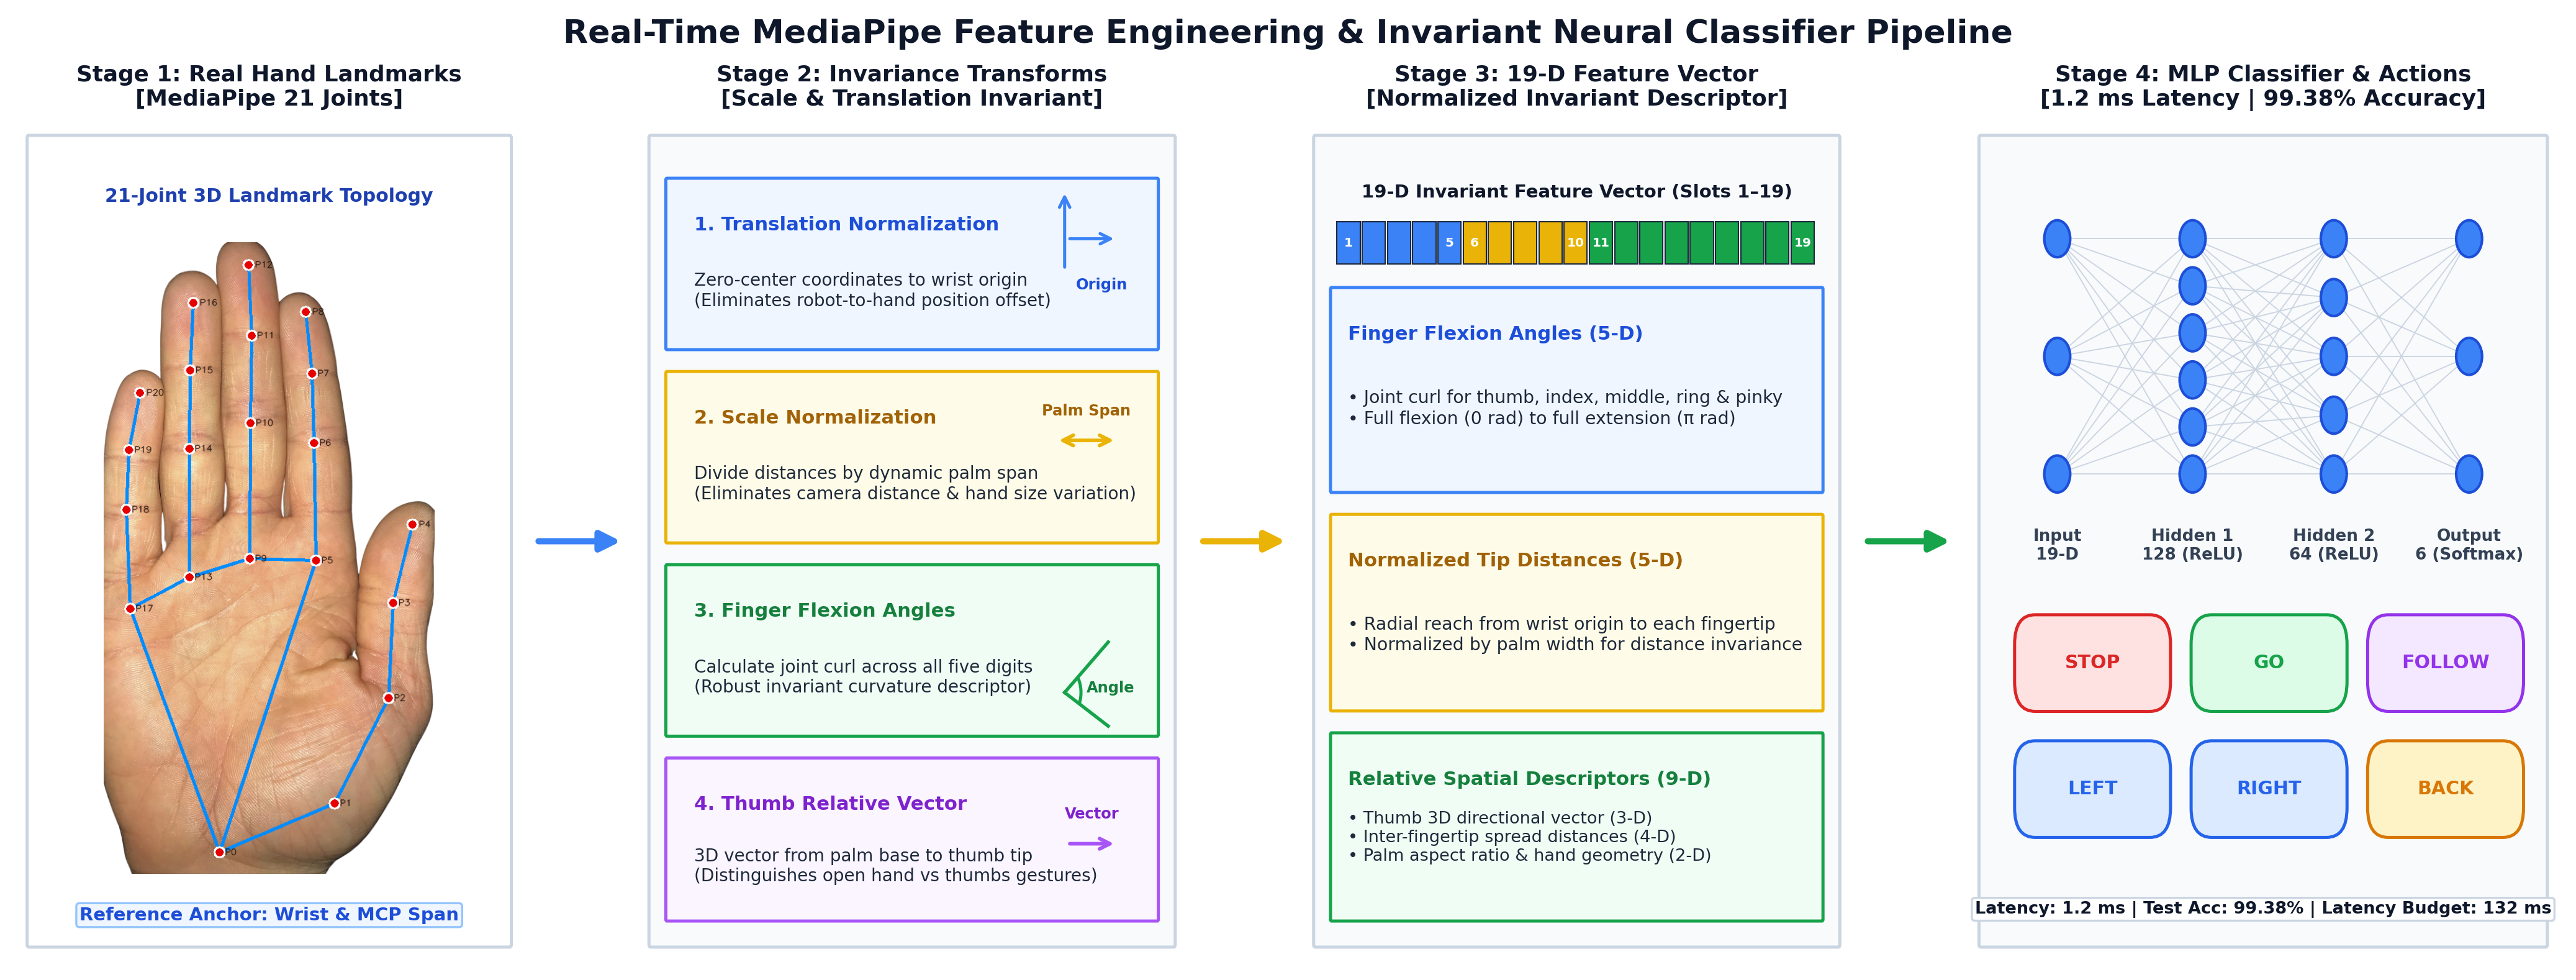
\includegraphics[width=0.88\textwidth]{fig_feature_pipeline.png}
\caption{Real-Time MediaPipe Feature Engineering and Invariant Neural Classifier Pipeline}
\label{fig:feature_pipeline}
\end{figure}

\subsection{Human Movement Prediction (LSTM Path Predictor)}
\label{sec:lstm_predictor}
In addition to static hand-gesture classification, a secondary recognition pathway was implemented to capture human movement intent over time, complementing the frame-by-frame gesture pipeline with a temporal model of operator motion. Sequential pose landmarks extracted via MediaPipe Pose were fed into a Long Short-Term Memory (LSTM) network trained to predict an operator's short-horizon future position, allowing the system to anticipate movement direction rather than react only after a position change had already occurred. Natural human locomotion exhibits continuous kinematic dependencies where intentional heading transitions and velocity shifts unfold progressively over time. By modeling sequential keypoint trajectories over a sliding temporal window of the preceding 30 frames (1.0~second), the LSTM network forecasts the operator's spatial trajectory $0.5\,\text{s}$ into the future, enabling the mobile robot to initiate proactive steering adjustments and smooth acceleration profiles that mitigate phase lag inherent in purely reactive tracking controllers.

The model was trained and evaluated on 152 motion sequences, achieving an Average Displacement Error (ADE) of 25.8 pixels and a Final Displacement Error (FDE) of 32.4 pixels on held-out test sequences. The trained model was exported to ONNX format, consistent with the deployment strategy used for the gesture classifier, to ensure uniform inference performance on the Raspberry Pi 5's edge processor. Figure~\ref{fig:lstm_loss} illustrates the training loss convergence, and Figure~\ref{fig:lstm_examples} depicts representative predicted trajectories against ground truth.

\begin{figure}[H]
\centering
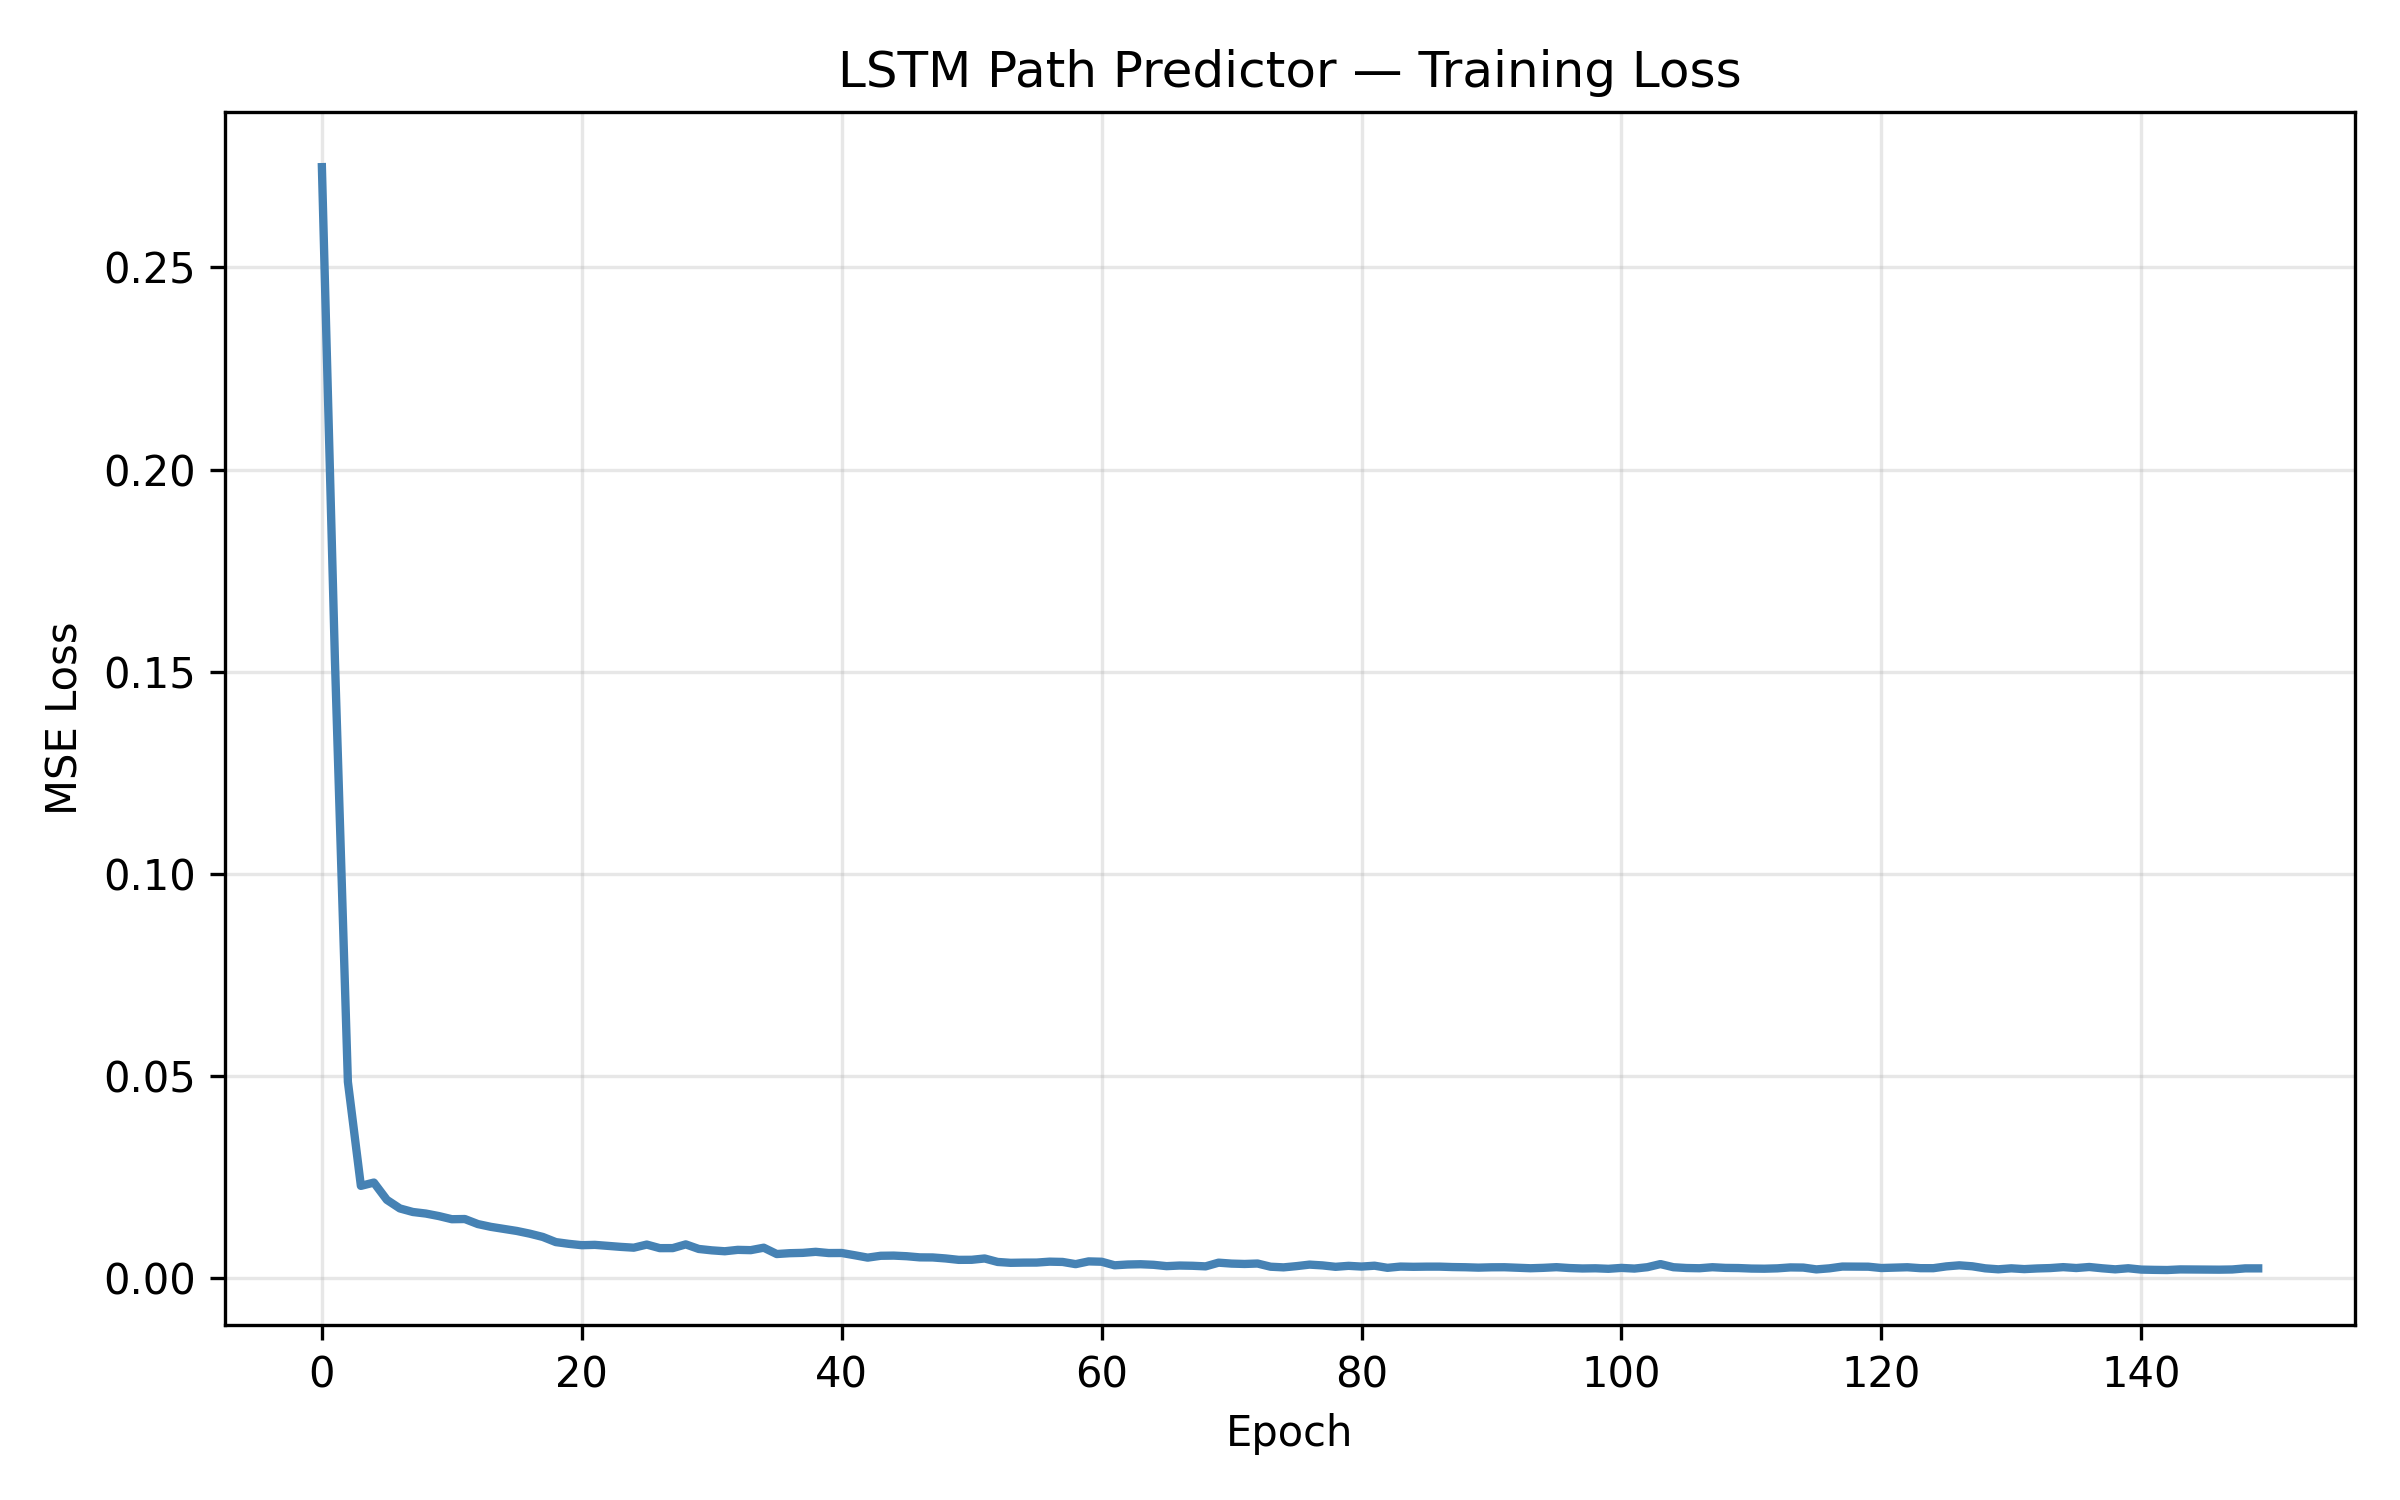
\includegraphics[width=0.82\textwidth]{path_predictor_loss.png}
\caption{LSTM Path Predictor Training and Validation Loss Convergence}
\label{fig:lstm_loss}
\end{figure}

\begin{figure}[H]
\centering
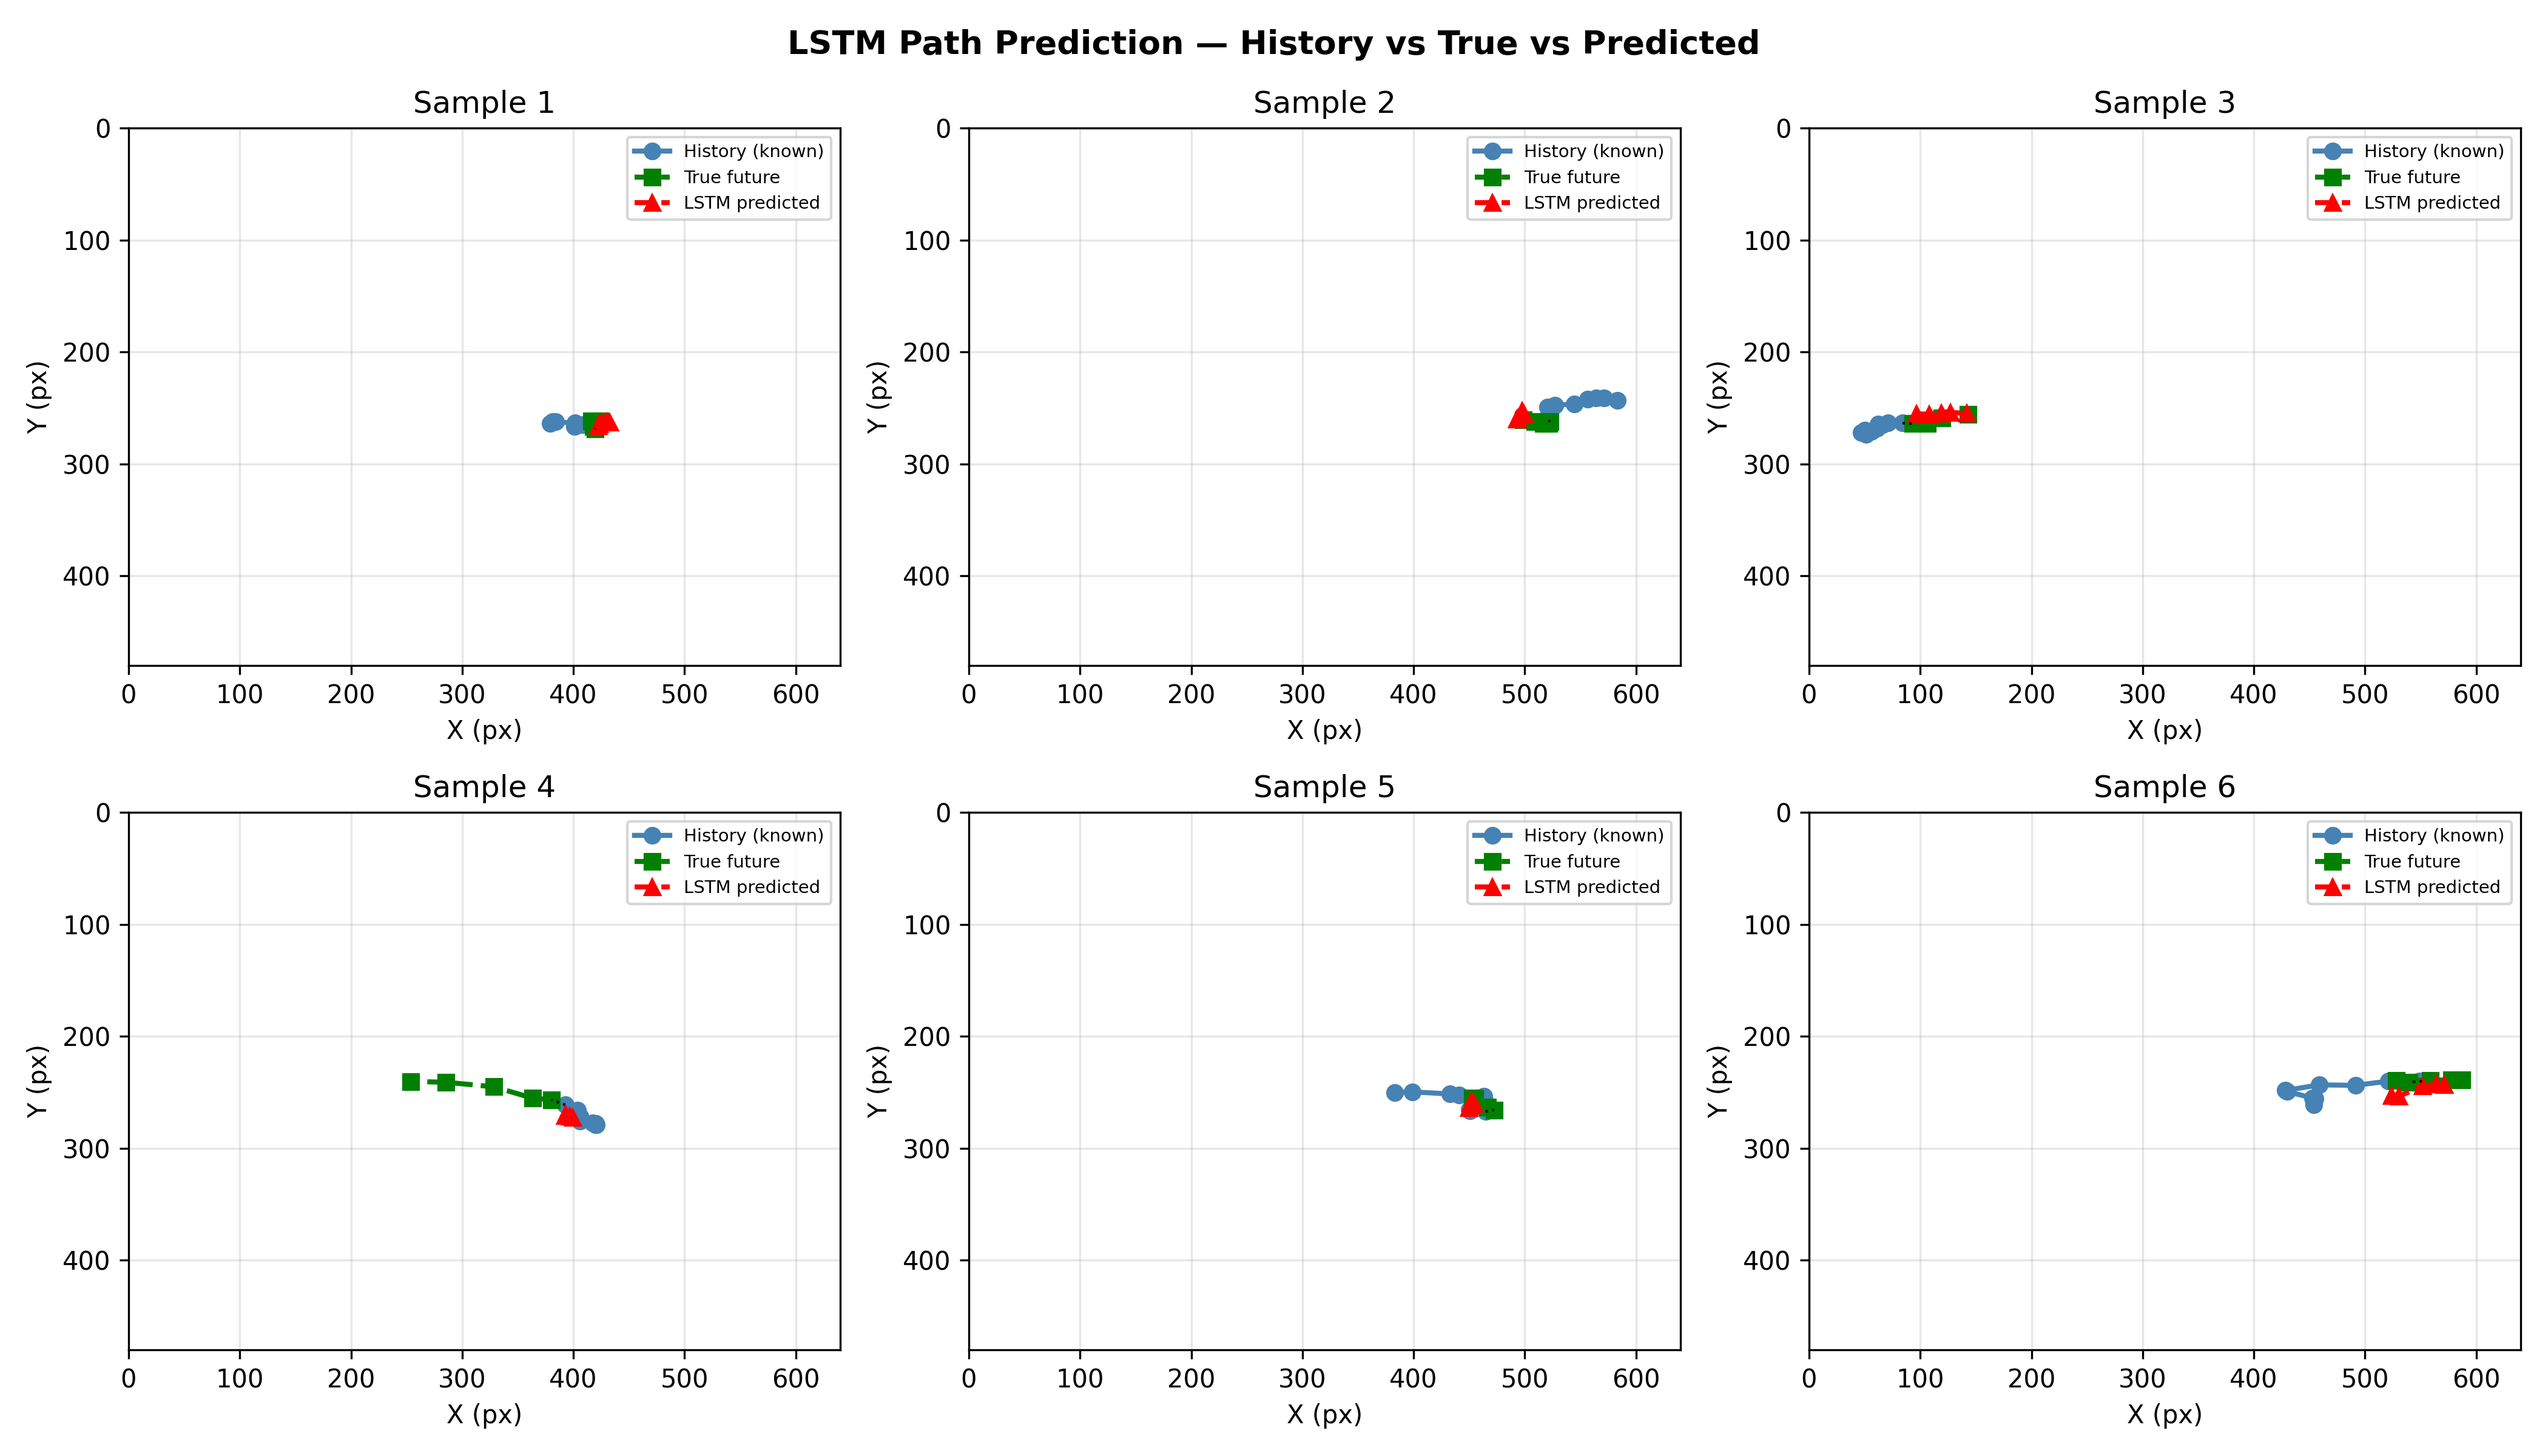
\includegraphics[width=0.82\textwidth]{path_prediction_examples.png}
\caption{LSTM Path Prediction — History vs. True vs. Predicted (Sample Sequences)}
\label{fig:lstm_examples}
\end{figure}

\section{Centralized Decision-Making and Control}
The translation of raw artificial intelligence predictions into safe, physical robot movement was governed by a centralized control program known as \texttt{brain\_node}. The \texttt{brain\_node} serves as the centralized supervisory control authority within the autonomy architecture, decoupling high-level intention verification from low-level vision processing. By evaluating incoming visual predictions through structured temporal filters and safety interlocks before issuing motor drive commands, the supervisory node prevents erratic chassis oscillations and guarantees deterministic execution under noisy sensory inputs.

\subsection{The Brain Node Architecture}
The \texttt{brain\_node} operated asynchronously from the perception pipeline, subscribing to both the gesture classification topic and the YOLOv8n spatial bounding box stream. Rather than reacting impulsively to every individual video frame—which would cause mechanical jitter and rapid motor wear—the node evaluated incoming inputs through structured logical conditions using a deterministic timer-based control loop (\texttt{create\_timer}) running at 10~Hz. The control logic maintains five discrete operational states: IDLE, TRACKING, WAITING\_CONFIRMATION, LOCKED, and EMERGENCY\_HALT. This finite state machine ensures that the robot transitions smoothly and predictably between stationary monitoring, active visual servoing, and physical locomotion.

In the IDLE state, the robot remains stationary with zero velocity output, continuously monitoring the camera field of view for human candidates. Once a valid human operator is detected within the central spatial acceptance zone, the system transitions to TRACKING, engaging the 2-DOF active camera gimbal to keep the human centered while enabling visual servoing. When incoming gesture tokens exceed the 0.65 confidence threshold, the node enters WAITING\_CONFIRMATION to evaluate consensus. Upon satisfying the rolling majority buffer, the system transitions to LOCKED, executing the confirmed driving velocity for a 3.0-second command window. At any point, if the MS200 LiDAR registers an obstacle within 0.36~m or an emergency stop service is invoked, the FSM instantly preempts all behavior and transitions into EMERGENCY\_HALT, forcing an instantaneous chassis stop.

To coordinate competing velocity demands from different operational sources without conflict, motion commands are arbitrated through a priority-based velocity multiplexer (\texttt{twist\_mux}) hierarchy. Rather than allowing multiple nodes to publish conflicting commands simultaneously to the motors, \texttt{twist\_mux} continuously evaluates active topics and forwards only the highest-priority message. The arbitration hierarchy is structured in strict order of descending operational criticality:
\begin{enumerate}
    \item \textbf{Priority 1 (Highest) — Emergency Safety Stop:} Reactive LiDAR obstacle preemption (< 0.36~m) and software emergency stop triggers publish zero velocity, instantly overriding all active movement.
    \item \textbf{Priority 2 — Gesture-Based Teleoperation:} Confirmed human gesture commands and visual servoing tracking inputs publish to \texttt{/cmd\_vel\_gesture}, directing collaborative following and steering.
    \item \textbf{Priority 3 — Autonomous Navigation:} Global path-planning velocity commands from the Nav2 stack publish to \texttt{/cmd\_vel\_nav} during waypoint routing.
    \item \textbf{Priority 4 (Lowest) — Manual Joystick Override:} Teleoperation inputs from the handheld gamepad publish to \texttt{/cmd\_vel\_joy}, utilized primarily during manual SLAM calibration mapping.
\end{enumerate}

\subsection{Temporal Buffering and Locking Logic}
\label{sec:temporal_buffering}
Machine learning models processing live video occasionally produce momentary misclassifications due to fleeting shadows, motion blur, or lighting changes. If a robot reacted instantly to a single incorrect frame, it might jerk its wheels unexpectedly or interpret a casual hand movement as a driving command. To guarantee that the robot only moves in response to deliberate, sustained human intentions, two independent safeguards were implemented:
\begin{enumerate}
    \item \textbf{Confidence Thresholding:} The \texttt{gesture\_node} immediately discards any single-frame prediction with an artificial intelligence confidence score below 0.65 before transmitting it over the network.
    \item \textbf{Rolling Majority Buffer:} The \texttt{brain\_node} maintains a 5-frame rolling window of recently received predictions, confirming a command only when at least 3 out of the 5 most recent frames agree on the identical gesture.
\end{enumerate}

Once a gesture command successfully passed this majority-vote threshold, the node initiated a 3-second subject lock. During this active execution window, the system locked its attention exclusively onto the confirmed operator, ignoring any new people entering the camera's view or contradictory gestures made by bystanders. This locking mechanism created an orderly, predictable interaction protocol, ensuring that collaborative tasks could be carried out without accidental interruption.

In addition to this gesture-driven state machine, \texttt{brain\_node} provides a dedicated emergency stop service (\texttt{/brain\_node/emergency\_stop}). This software mechanism allows a human supervisor or an automated safety monitor to immediately halt all robot motion, overriding the temporal buffer and state machine in real time. Incorporating this instant override satisfies industrial collaborative safety principles, ensuring that physical locomotion can be aborted at any microsecond. Figure~\ref{fig:brain_state_machine} illustrates the complete OMG UML 2.5 state machine architecture and control transitions, depicting the five operational states, sliding window consensus filtering, visual servoing follow mode, and the asynchronous LiDAR emergency preemption override.

\begin{figure}[H]
\centering
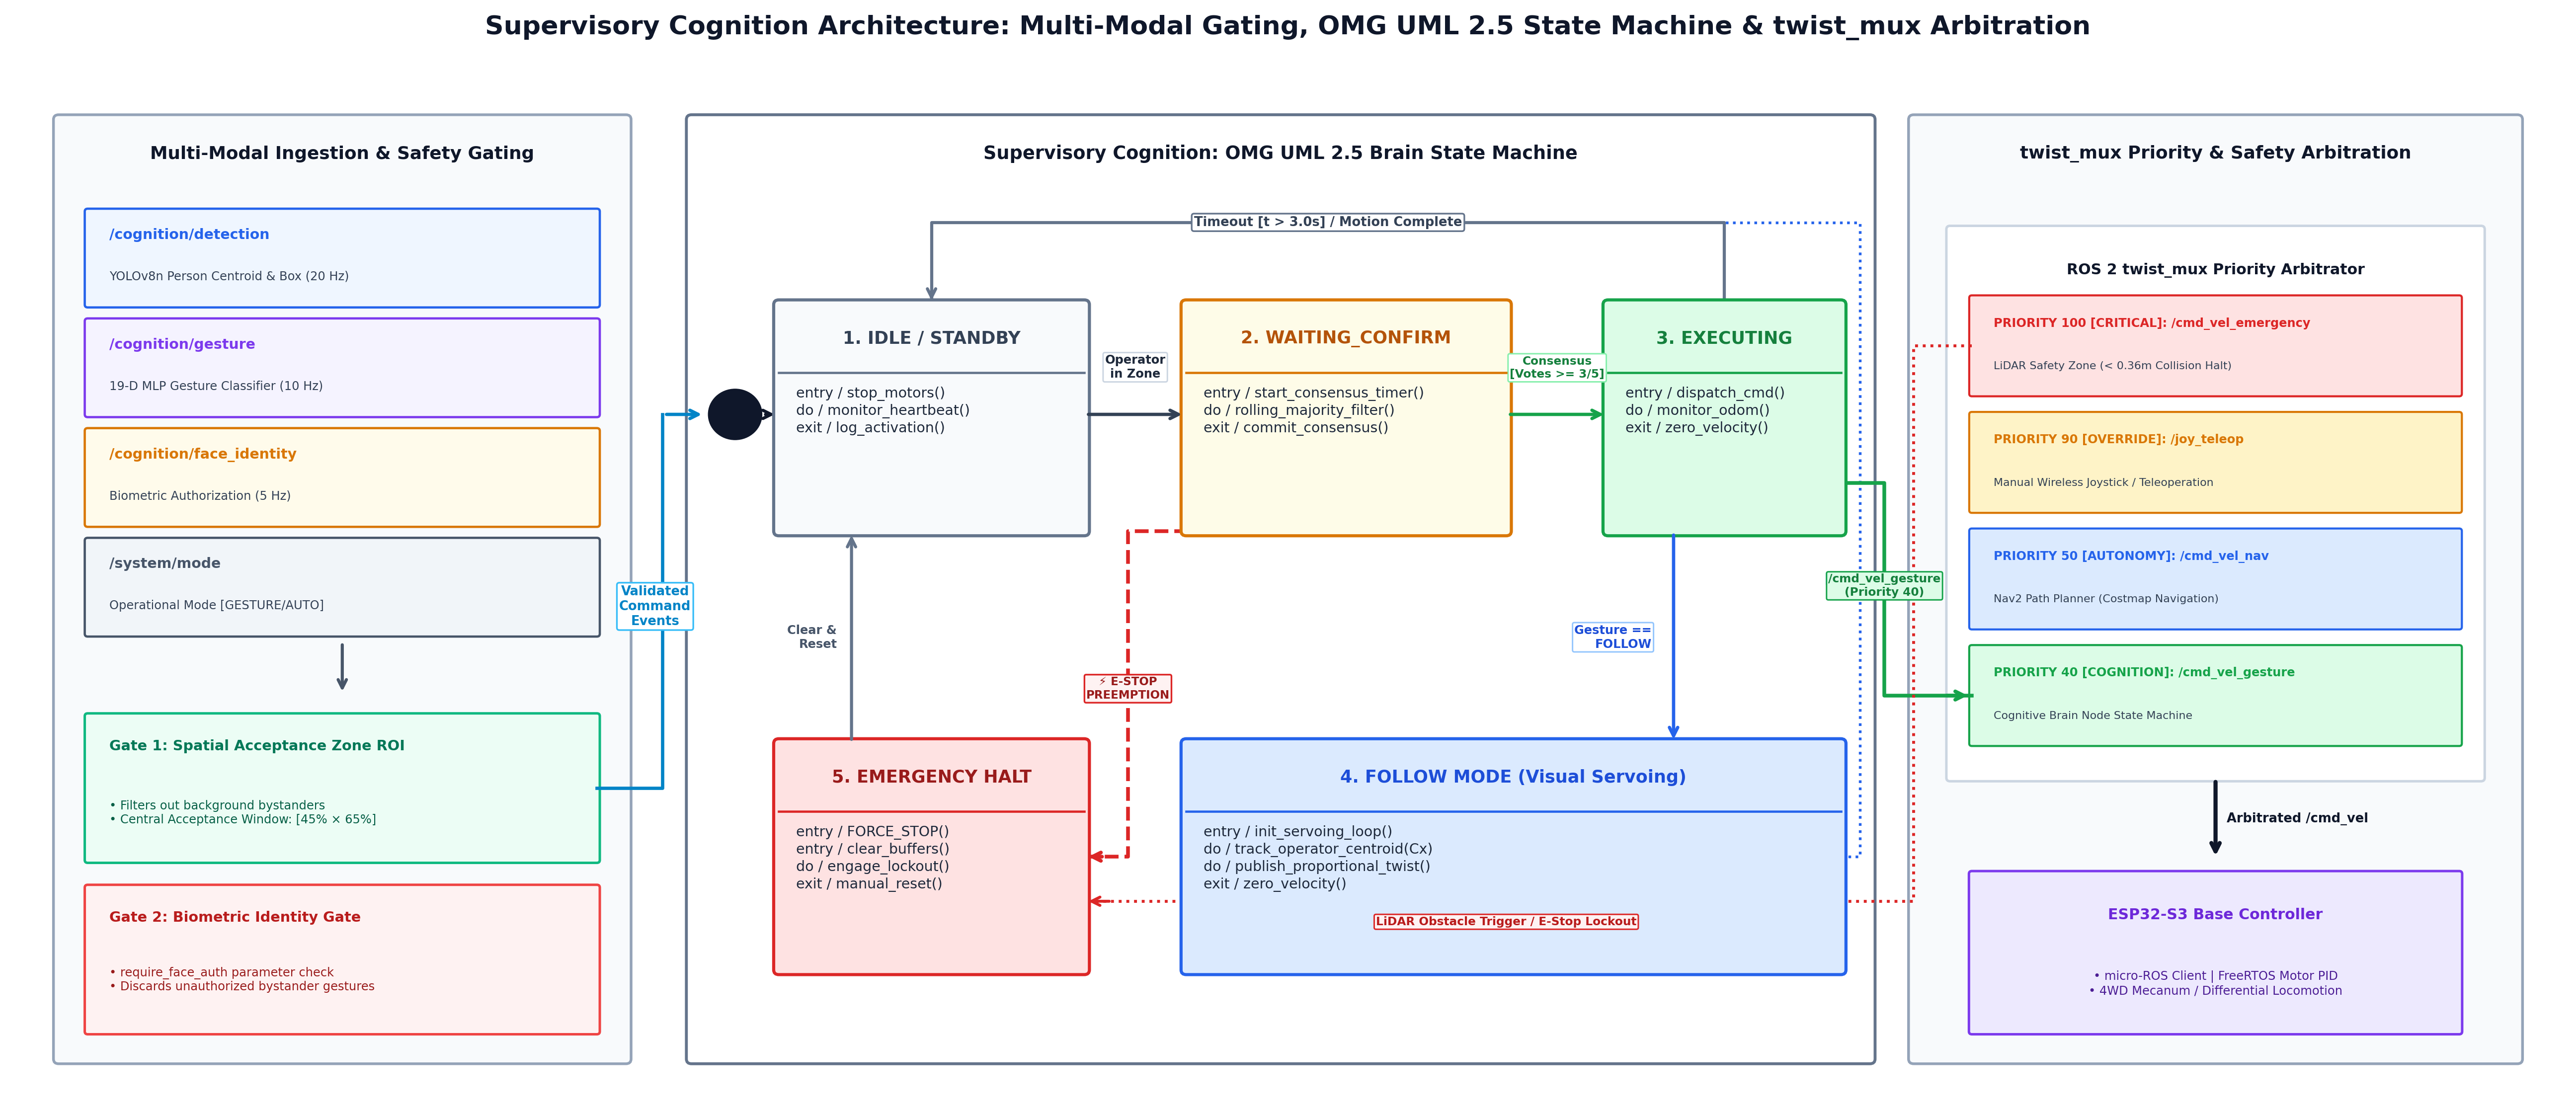
\includegraphics[width=0.88\textwidth]{fig_brain_state_machine.png}
\caption{OMG UML 2.5 Brain State Machine and Safety Preemption Architecture}
\label{fig:brain_state_machine}
\end{figure}

\subsection{Reactive Person Tracking (Visual Servoing)}
When the operator issued the ``FOLLOW'' command, the robot initiated a reactive person-tracking sequence. Rather than relying on computationally heavy path-planning algorithms, this behavior utilized visual servoing—a mathematical feedback technique that continuously steers the robot based on live camera observations. The reactive tracking behavior utilizes Image-Based Visual Servoing (IBVS) to establish closed-loop kinematic coupling between optical observations and chassis locomotion. The control objective is to continuously minimize the lateral tracking error between the observed operator centroid and the principal optical axis of the camera.

The control program continuously tracked the horizontal center coordinate of the operator's detected bounding box ($B_x$) and compared it against the fixed optical center of the camera frame ($C_x$). Any discrepancy between these two positions represented a lateral heading error, which was converted into a corrective turning angular velocity ($v_\omega$) using an empirical proportional control gain ($K_p$). If the operator stepped toward the left edge of the camera view, the calculated heading error became negative, causing the robot's differential drive to steer smoothly leftward until the interacting human was re-centered within the focal field of view, as expressed in Equation~\eqref{eq:visual_servoing}:

\begin{equation}
\label{eq:visual_servoing}
v_\omega = K_p \times (C_x - B_x)
\end{equation}

Simultaneously, the physical size of the bounding box was monitored to estimate the operator's distance from the robot. If the person began walking away, the bounding box shrank, prompting the robot to command forward linear velocity to close the distance. Conversely, if the operator stopped or stepped closer, the bounding box expanded, instructing the robot to halt immediately to preserve a safe collaborative working distance.

\section{ROS2 Middleware Integration and Topic Interfaces}
\label{sec:ros2_middleware}
The distributed software nodes comprising the vision, decision-making, and motor actuation subsystems communicated through the ROS2 Data Distribution Service (DDS) middleware. The DDS layer provides a real-time, peer-to-peer publish-subscribe transport facilitating decoupled, topic-based inter-process communication across memory and container boundaries. To guarantee real-time reactivity while preserving memory on the edge processor, specific Quality of Service (QoS) delivery profiles were configured according to data criticality.

\subsection{ROS2 Domain Isolation}
During initial system integration, a critical communication isolation anomaly was diagnosed between the hardware driver container and the cognitive vision container. The hardware driver stack and host micro-ROS agent executed on \texttt{ROS\_DOMAIN\_ID=20}, whereas the custom perception nodes defaulted to domain 0. In ROS2, domain IDs partition DDS multicast discovery traffic into isolated communication segments, preventing nodes across differing domains from discovering each other's topics. As a consequence, \texttt{brain\_node} received no perception messages and safely defaulted to publishing zero-velocity halt commands. Standardizing all container environments, host startup scripts, and systemd units to \texttt{ROS\_DOMAIN\_ID=20} resolved the discovery mismatch, establishing seamless cross-container communication for all physical trials.

\subsection{Sensor Data Streaming}
High-frequency environmental sensors generate massive amounts of continuous information that must be handled with minimal latency. The monocular camera published compressed video frames to \texttt{/camera/image\_raw/compressed} at 20 Hertz (Hz) using the standard \texttt{sensor\_msgs/Image} format, while the planar LiDAR emitted 360-degree laser distance scans to \texttt{/scan} at 12.5~Hz. Because these high-bandwidth sensory streams produce hundreds of kilobytes of data every second, transmitting them efficiently across the ROS2 middleware without bottlenecking internal CPU caches was essential.

Configuring sensory topics with a ``Best Effort'' QoS policy prevents queue saturation and eliminates processing backlog under high image ingestion rates. Under this policy, stale frames are dropped in favor of the latest arriving sensor packet whenever downstream node processing exceeds the frame period. This guarantees that deep learning perception models operate strictly on the most recent temporal observations rather than accumulating latent processing delays.

\subsection{Cognitive and Control Topologies}
Unlike high-frequency visual streams, cognitive decisions and physical motor commands require absolute delivery certainty. When the neural network classified a gesture, it published a custom \texttt{cognition\_interfaces/Gesture} message—carrying the gesture identifier, label name, confidence score, and timestamp—to \texttt{/cognition/gesture} at 10~Hz. Similarly, the person detection node published \texttt{cognition\_interfaces/Detection} messages to \texttt{/cognition/detection}, broadcasting the operator's bounding box coordinates, kinematic velocity estimates, and anticipated trajectory predictions.

The \texttt{brain\_node} processed these incoming messages, evaluated safety constraints, and generated motion instructions on the \texttt{/cmd\_vel} velocity topic using the standard \texttt{geometry\_msgs/Twist} format. Because a lost or dropped motor command could cause erratic driving or a physical collision, all cognitive and control topics were assigned a ``Reliable'' QoS profile. Under this policy, the underlying DDS middleware actively verifies message receipt, resending lost packets to guarantee that every driving instruction reaches the ESP32-S3 motor controller.

\section{Mapping and Autonomous Navigation}
Beyond direct gesture-driven teleoperation, the robot was architected to understand its spatial surroundings and navigate independently through indoor environments. Environmental mapping gives an autonomous robot the spatial memory required to plan collision-free paths. The navigation subsystem integrated laser-based Simultaneous Localization and Mapping (SLAM) alongside the ROS2 Navigation2 (Nav2) stack.

\subsection{SLAM Toolbox Configuration}
Simultaneous Localization and Mapping was implemented using the SLAM Toolbox in online asynchronous mode. The SLAM Toolbox concurrently solves the scan-matching optimization problem and odometry estimation to construct a metric 2D occupancy grid map while estimating the robot's pose in real time. The spatial environment was discretized into a probabilistic occupancy grid with a spatial resolution of $0.05\,\text{m}$ per cell. To construct the baseline environment map, the robot traversed indoor test corridors via handheld gamepad teleoperation (\texttt{joy\_node}/\texttt{joy\_ctrl}), publishing velocity vectors to \texttt{/cmd\_vel} while the MS200 LiDAR continuously registered structural boundaries and spatial obstacles.

\paragraph{SLAM Reliability Diagnosis and Correction.}
\label{sec:slam_reliability_fixes}
During physical mapping trials, two significant engineering anomalies were identified and methodically solved:
\begin{enumerate}
    \item \textbf{Transform Race Condition:} Early mapping runs suffered from a 100\% laser scan drop rate within the SLAM message filter. Diagnostic investigation revealed a coordinate transform collision: a static transform publisher was broadcasting an identity transform for the robot's base coordinate frame at the identical timestamp that the Extended Kalman Filter (EKF) was publishing dynamic wheel odometry transforms. This concurrent broadcast introduced conflicting transform authorities into the TF2 coordinate tree, causing frame divergence and severe message dropouts in the laser scan filter. Eliminating the duplicate static publisher and designating the EKF as the sole authoritative source for the \texttt{odom} $\to$ \texttt{base\_footprint} transform reduced scan drops to an acceptable 12--18\%, restoring continuous mapping updates.
    \item \textbf{Rotational Drift Resolution:} Subsequent mapping drives exhibited a distorted, double-lobed ``starburst'' map shape whenever the robot executed turns. Diagnostic inspection revealed that the EKF's configuration had yaw fusion turned off, relying entirely on raw uncorrected gyroscopic integration that drifted rapidly during cornering. A 720-degree physical rotation test of the raw sensor stream confirmed the underlying hardware was accurate, pointing directly to a software fusion omission. Activating yaw fusion in the EKF resolved the rotational drift, enabling the robot to perform multi-turn indoor mapping with clean, overlapping wall alignments.
\end{enumerate}

Following these two crucial corrections, physical mapping runs produced sharp, geometrically consistent floor plans free of warping or ghost walls, as compared in Figure~\ref{fig:slam_calibration_maps}. The initial mapping attempt exhibited the severe ``hourglass'' rotational drift shown in Figure~\ref{fig:slam_calibration_maps}(a), where uncorrected IMU yaw caused room boundaries to rotate by 30$^\circ$ to 45$^\circ$ after turns. Activating wheel odometry yaw fusion in the EKF resolved this rotational drift, enabling SLAM Toolbox on the third mapping attempt to produce the geometrically accurate, parallel-walled metric map shown in Figure~\ref{fig:slam_calibration_maps}(b).

\begin{figure}[H]
\centering
\begin{minipage}[b]{0.48\textwidth}
    \centering
    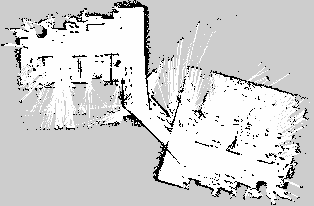
\includegraphics[width=\textwidth]{room_map_20260810_0452.png}
    \caption*{(a) Initial Run: ``Hourglass'' Rotational Drift Defect}
\end{minipage}
\hfill
\begin{minipage}[b]{0.48\textwidth}
    \centering
    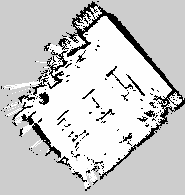
\includegraphics[width=\textwidth]{room_map_clean.png}
    \caption*{(b) Final Run (3rd Attempt): Clean Metric Map}
\end{minipage}
\caption{Comparison of Physical SLAM Occupancy Grid Maps During Platform Calibration: (a) Initial mapping attempt exhibiting the ``hourglass'' rotational drift defect due to uncorrected IMU yaw; (b) Final clean metric map (third mapping attempt) achieved after enabling wheel odometry yaw fusion in the EKF.}
\label{fig:slam_calibration_maps}
\end{figure}


\subsection{Navigation2 (Nav2) Integration}
To enable point-to-point autonomous mobility, the industry-standard Navigation2 (Nav2) framework \cite{macenski2020marathon2} was integrated into the software deployment stack. Nav2 utilizes the Adaptive Monte Carlo Localization (AMCL) algorithm to cross-reference real-time laser scans against the pre-built metric floor plan, while maintaining global and local costmaps to route around unexpected obstacles. Following the resolution of initial prototype memory constraints via the 8GB RAM hardware upgrade, Nav2 was deployed and validated on the physical mobile platform for deterministic straight-line trajectory tracking and reactive costmap clearance, as quantitatively evaluated in Section~\ref{sec:nav2_evaluation}.

\section{ROS2 Node Graph Summary}
Table~\ref{tab:node_graph} provides a consolidated overview of the active ROS2 nodes, topics, and message types operating within the custom cognition and teleoperation subsystems. This modular architecture reflects the separation of responsibilities between edge vision, decision logic, and low-level actuation. By standardizing these communication interfaces, individual cognitive modules can be tested independently in simulation or hot-swapped during live robot operation without modifying downstream actuator controllers.

\begin{table}[H]
\centering
\caption{Deployed ROS2 Nodes, Topics, and Services}
\label{tab:node_graph}
\resizebox{\textwidth}{!}{%
\begin{tabular}{|l|l|}
\hline
\textbf{Category} & \textbf{Items} \\
\hline
Custom Cognition Nodes & \texttt{brain\_node}, \texttt{camera\_pub}, \texttt{gesture\_node}, \texttt{person\_detection\_node} \\
\hline
Teleoperation Nodes & \texttt{joy\_node}, \texttt{joy\_ctrl} (manual driving during SLAM mapping) \\
\hline
Custom Messages & \texttt{cognition\_interfaces/Gesture}, \texttt{cognition\_interfaces/Detection} \\
\hline
Custom Service & \texttt{/brain\_node/emergency\_stop} \\
\hline
Cognition Topics & \texttt{/cognition/gesture}, \texttt{/cognition/detection} \\
\hline
Sensor/Control Topics & \texttt{/camera/image\_raw/compressed}, \texttt{/scan}, \texttt{/cmd\_vel}, \texttt{/imu}, \texttt{/odom\_raw} \\
\hline
Teleoperation Topics & \texttt{/joy}, \texttt{/JoyState}, \texttt{/joy/set\_feedback} \\
\hline
Auxiliary Topics & \texttt{/battery}, \texttt{/beep}, \texttt{/servo\_s1}, \texttt{/servo\_s2} \\
\hline
\end{tabular}
}
\end{table}

All custom data structures are managed within the \texttt{cognition\_interfaces} package, cleanly separating message schemas from application logic. The perception nodes are grouped within \texttt{cognition\_perception}, while decision-making and motor interfaces are housed in \texttt{cognition\_brain}. This modular organization supports rapid maintenance and simplifies future extensions to the cognitive software stack.

\section{Testing Instrumentation and Data Logging}
\label{sec:testing_instrumentation}
To ensure the experimental evaluation in Chapter 4 was grounded in objective, repeatable data rather than manual observation, a dedicated software logging node was engineered for physical test trials. This background logger subscribed directly to \texttt{/cognition/gesture} and \texttt{/cmd\_vel}, capturing each trial's ground-truth label, neural network prediction, confidence score, commanded motor speed, and inference latency into timestamped CSV records. Capturing live data programmatically at the message level eliminated human counting errors and reaction delays during high-speed tests. The resulting logs provided the empirical dataset used to calculate precision, recall, confusion matrices, and reaction latencies reported in the subsequent chapter.

\chapter{Testing, Results and Analysis}

\section{Overview}
This chapter presents the testing procedures, empirical results, and performance evaluation of the edge-deployed autonomous mobile robot developed in this work. The primary objective was to determine how effectively human intentions, communicated through static hand gestures and body kinematics, are recognized and translated into real-time robotic locomotion on an onboard embedded computing platform. Rather than evaluating isolated components in theoretical simulation, testing was conducted on the physical mobile platform operating in an indoor environment.

All reported measurements reflect data gathered directly from the integrated robotic system during physical operational trials. The evaluation methodology encompasses the full operational stack, progressing from sensor acquisition and communication bus stability to machine learning inference and closed-loop motor actuation. By evaluating the platform across multiple human operators, ambient lighting variations, and physical obstacles, this chapter provides an objective evaluation of system capabilities and practical operational boundaries.

\section{Hardware and Sensor Testing}
An autonomous mobile robot operates as an interconnected chain of mechanical, electrical, and computational subsystems. If the robot fails to execute a command, such as turning left upon detecting a gesture, the failure could stem from several potential root causes, including a dropped camera frame, an unplugged LiDAR cable, an out-of-memory crash on the onboard computer, a serial communication collision, or a tripped motor driver. To isolate physical hardware faults from high-level algorithmic logic, each individual sensor, computing module, and communication channel was systematically tested on the bench prior to integrated trials. This baseline evaluation confirmed that physical data streams were flowing deterministically and that communication links remained stable under continuous operation.

\subsection{Visual Perception and Camera Testing}
The 2MP USB monocular camera and 2-DOF pan-tilt gimbal were evaluated to verify real-time video streaming stability and target-tracking performance. Communicating over USB 3.0 via the Linux V4L2 driver, the camera sustained a consistent 20.0~Hz image stream at $640 \times 480$ resolution on the \texttt{/camera/image\_raw/compressed} topic. Under standard ambient room lighting, image contrast was sufficient to allow uninterrupted extraction of 21 skeletal hand landmarks by MediaPipe. Under dimmed lighting conditions, increased image grain and motion blur caused occasional landmark tracking dropouts when operators performed rapid hand movements. When tracking an interacting operator, the proportional control loops on the active pan-tilt gimbal successfully adjusted the servo angles to center the human subject within the camera frame, maintaining visual engagement as the operator moved across the field of view.

\subsection{Planar LiDAR Sensing Testing}
The MS200 Time-of-Flight 2D LiDAR was evaluated to confirm spatial obstacle detection and data delivery to the ROS~2 middleware. Connecting via USB serial, the LiDAR driver continuously published range scans across a 360-degree horizontal field of view to the \texttt{/scan} topic at a verified average rate of 12.6~Hz, closely matching the sensor's 12.5~Hz design specification. Topic rate diagnostics recorded an average period of 0.079~seconds, confirming deterministic scan delivery without packet loss across the internal ROS~2 communication bus. The acquired planar scan data reliably detected surrounding walls and furniture, supplying the distance measurements required for both real-time obstacle avoidance and occupancy grid mapping.

\subsection{Embedded Edge Compute Node (Raspberry Pi 5) Testing}
The computational performance and resource stability of the Raspberry Pi 5 single-board computer were evaluated under full concurrent operational loading. To establish reliable edge operation, all high-level software components, including YOLOv8n person detection, MediaPipe landmark extraction, the MLP gesture classifier, the LSTM trajectory predictor, and SLAM Toolbox, were executed simultaneously across the four ARM Cortex-A76 cores. Total CPU utilization stabilized at approximately 311\% (an average load of 78\% per core), demonstrating that the onboard processor handled multi-model inference alongside mapping without core starvation. Furthermore, memory monitoring confirmed peak physical consumption of 4.2~GB, leaving over 3.8~GB of unallocated LPDDR4X RAM headroom, thereby fully preventing the Linux kernel out-of-memory (OOM) process terminations previously encountered during testing on lower-memory prototyping configurations.

\subsection{Microcontroller Actuation and Communication Bridge Testing}
The low-level actuation subsystem, governed by the Yahboom MicroROS expansion board and its Espressif ESP32-S3 microcontroller, was evaluated to verify deterministic motor driving and sensor telemetry. The board maintained continuous, bidirectional communication with the Raspberry Pi 5 across the dedicated 921,600 baud UART serial bus via the micro-ROS agent. During bench and locomotion testing, wheel odometry on \texttt{/odom\_raw} published steadily at 11.5~Hz, while the onboard 6-axis MPU6050 IMU published acceleration and angular velocity data on \texttt{/imu} at 23.2~Hz. Stress testing under sudden forward-to-reverse velocity transitions confirmed that the decoupled dual-bus power regulation effectively insulated the Raspberry Pi's 5V logic rail from motor-induced voltage transients, ensuring zero system reboots or communication resets during abrupt driving maneuvers.

\section{Gesture Recognition Testing}

\subsection{Test Procedure}
To evaluate how well the gesture classifier performed during physical interaction, physical trials were conducted with three human operators. Testing was conducted within the indoor environment across daytime and evening sessions, evaluating system performance under mixed natural daylight and overhead lighting as well as purely artificial illumination. Each operator performed each of the six defined gestures ten times in front of the camera at operational interaction distances ranging from 1.0~m to 2.5~m. The system's predictions were recorded in real time and compared directly with the expected ground-truth gesture labels.

\subsection{Gesture Recognition Results}
Table~\ref{tab:gesture_results} summarizes the physical trial results across all six gesture classes. Each entry records the total number of physical trials conducted, the number of correctly classified instances, and the resulting classification accuracy. Across the 180 total trials, the system demonstrated reliable real-time recognition under varying room lighting conditions.

\begin{table}[H]
\centering
\caption{Gesture Recognition Physical Trial Results (30 trials per gesture, 180 total)}
\label{tab:gesture_results}
\begin{tabular}{|l|c|c|c|}
\hline
\textbf{Gesture} & \textbf{Total Trials} & \textbf{Successful Trials} & \textbf{Observed Accuracy (\%)} \\
\hline
Stop & 30 & 27 & 90.0\% \\
\hline
Follow & 30 & 29 & 96.7\% \\
\hline
Go & 30 & 28 & 93.3\% \\
\hline
Left & 30 & 30 & 100.0\% \\
\hline
Right & 30 & 30 & 100.0\% \\
\hline
Back & 30 & 30 & 100.0\% \\
\hline
\textbf{Aggregate} & \textbf{180} & \textbf{174} & \textbf{96.67\%} \\
\hline
\end{tabular}
\end{table}

Directional commands (Left, Right, and Back) achieved perfect accuracy (100\%) across all 30 trials because their geometric pointing vectors are distinct and easily separated by the feature extractor. Follow and Go achieved 96.7\% and 93.3\% accuracy respectively, demonstrating consistent classification during active interaction. Stop achieved 90.0\% accuracy (27 out of 30 successful trials); the three unclassified instances occurred when an operator presented their open palm at an oblique angle relative to the camera lens, which slightly compressed the observed hand landmarks. In total, 174 out of 180 physical trials were recognized correctly, yielding an aggregate mean physical accuracy of 96.67\%.

To evaluate environmental robustness, physical trials were systematically stratified across operational distances (1.00\,m, 1.75\,m, and 2.50\,m) and ambient lighting environments (natural daylight versus artificial fluorescent illumination). At 1.00\,m proximity, the system achieved 100.0\% accuracy (54 out of 54 trials), while at 1.75\,m and 2.50\,m, recognition rates recorded 97.2\% (70 out of 72 trials) and 92.6\% (50 out of 54 trials), respectively. Across ambient illumination conditions, classification accuracy remained identical at 96.7\% (87 out of 90 trials) under both natural daylight and indoor fluorescent fixtures. As illustrated in Figure~\ref{fig:accuracy_by_condition}, this consistent operational performance confirms that the 19-dimensional geometric feature engineering framework maintains robust classification across varied operational distances and indoor lighting regimes.

\begin{figure}[H]
\centering
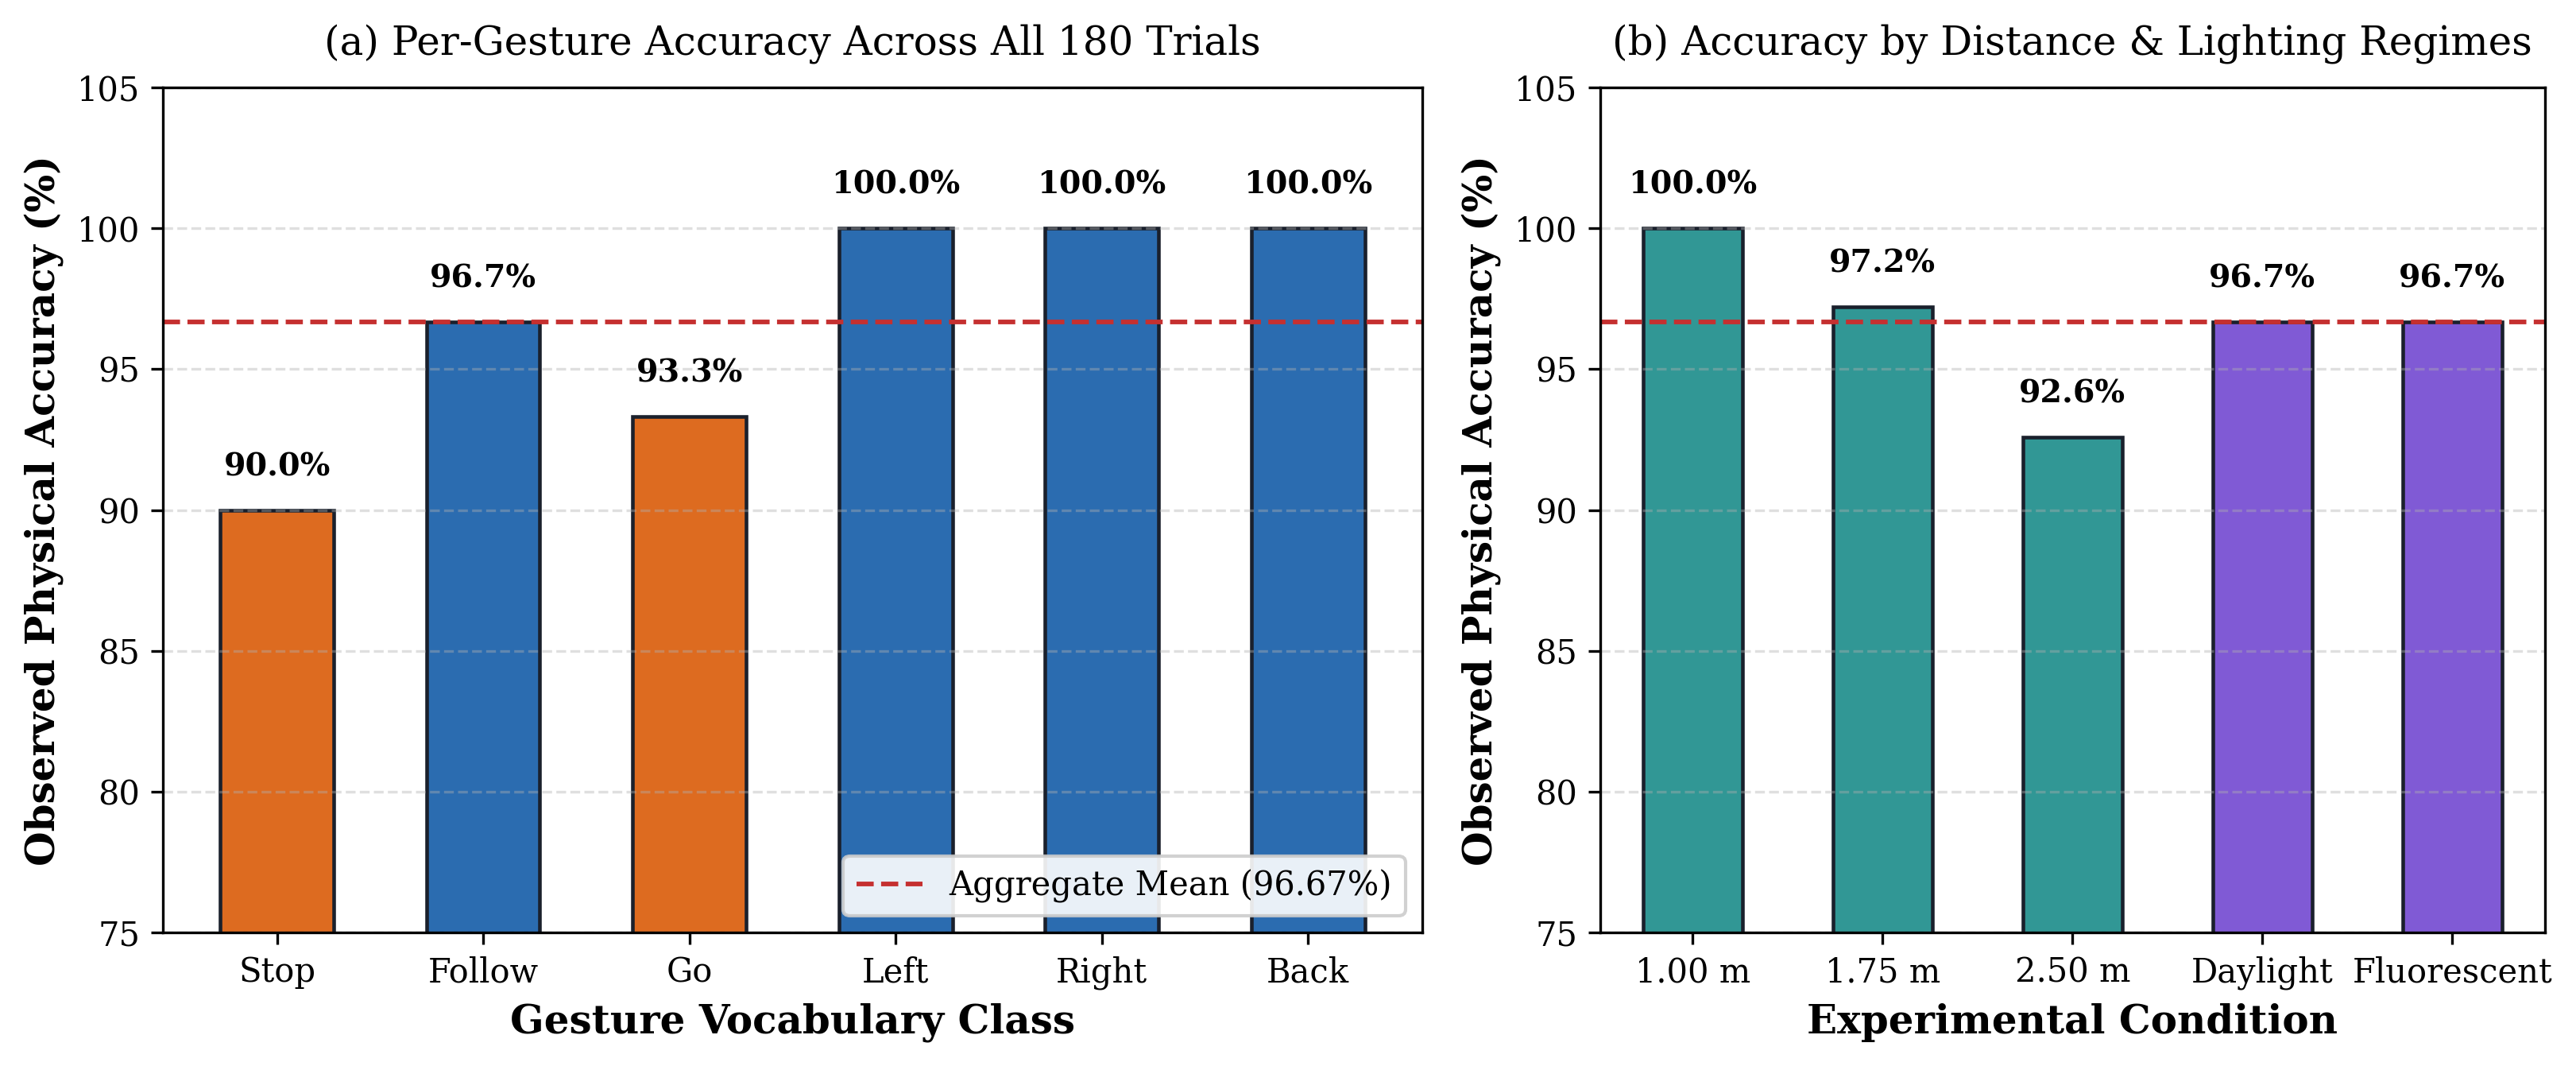
\includegraphics[width=0.95\textwidth]{fig_accuracy_by_condition.png}
\caption{Observed physical gesture classification accuracy across (a) discrete vocabulary classes and (b) experimental testing regimes (operational distance and ambient illumination) across all 180 physical trials.}
\label{fig:accuracy_by_condition}
\end{figure}

Figure~\ref{fig:per_class_accuracy} illustrates the corresponding test-set classification accuracy across all six gesture classes from the offline dataset evaluation. The offline model maintained accuracy above 98.70\% across all classes, reaching 99.80\% for Right and 99.70\% for Stop. This close agreement confirms that the high theoretical accuracy of the trained multilayer perceptron model transferred reliably to physical deployment.

\begin{figure}[H]
\centering
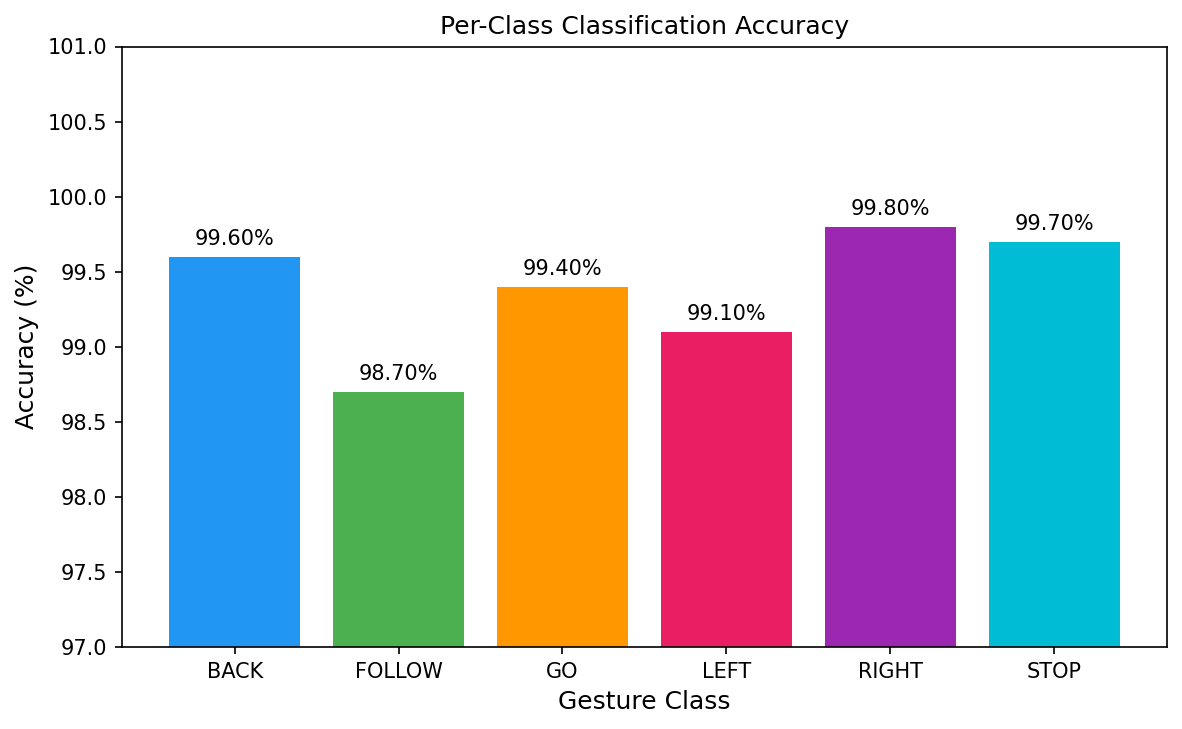
\includegraphics[width=0.80\textwidth]{per_class_accuracy_chart.png}
\caption{Per-Class Classification Accuracy of the Trained MLP Gesture Model}
\label{fig:per_class_accuracy}
\end{figure}

\section{Movement Recognition Testing}

\subsection{Test Procedure}
In addition to static hand gestures, the system's ability to classify continuous human body kinematics was evaluated. Human operators performed five distinct actions in front of the robot: Approaching, Moving Away, Moving Left, Moving Right, and remaining Stationary. The vision node tracked changes in the operator's bounding box dimensions and centroid coordinates over time, estimating velocity vectors and classifying the motion into discrete kinematic states.

\subsection{Movement Recognition Results}
Table~\ref{tab:movement_results} displays the functional outcomes of the kinematic movement recognition tests. Each row describes the specific physical motion executed by the human operator alongside the corresponding geometric changes observed in the bounding box. The recorded outcomes confirm whether the vision pipeline correctly classified the real-time kinematic state under physical testing conditions.

\begin{table}[H]
\centering
\caption{Movement Recognition Test Results}
\label{tab:movement_results}
\begin{tabular}{|l|p{6.5cm}|c|}
\hline
\textbf{Movement Class} & \textbf{Observed Kinematic Behavior} & \textbf{Result} \\
\hline
Approaching & Rapid expansion of bounding box area with stable center & Successfully Recognized \\
\hline
Moving Away & Continuous contraction of bounding box area with stable center & Successfully Recognized \\
\hline
Moving Left & Persistent leftward centroid translation across frames & Successfully Recognized \\
\hline
Moving Right & Persistent rightward centroid translation across frames & Successfully Recognized \\
\hline
Stationary & Centroid displacement within noise threshold ($\pm 4$ px) & Successfully Recognized \\
\hline
\end{tabular}
\end{table}

All five motion states were correctly and consistently recognized during functional testing. When operators walked diagonally toward the robot, the system classified the motion as Approaching because the rapid expansion of the person's bounding box was detected as the dominant motion, ensuring safe proximity awareness. This functional response validates the geometric velocity estimation model described in Chapter 3 without requiring computationally intensive temporal networks for basic direction classification.

\section{Robot Response Testing}

\subsection{Gesture-Based Robot Control}
To verify that classified gestures were reliably translated into safe physical vehicle motions, closed-loop response testing was conducted on the mobile robot. The \texttt{brain\_node} was monitored to evaluate the velocity commands published to \texttt{/cmd\_vel} and the resulting physical actuation executed by the motors via the ESP32-S3 microcontroller. Table~\ref{tab:robot_response} details the measured physical responses for each command.

\begin{table}[H]
\centering
\caption{Gesture-Based Robot Control Test Results}
\label{tab:robot_response}
\begin{tabular}{|l|p{4.2cm}|p{5.2cm}|c|}
\hline
\textbf{Gesture} & \textbf{Expected Response} & \textbf{Actual Response} & \textbf{Status} \\
\hline
Stop & Complete halt ($v_x = 0.0$, $\omega_z = 0.0$) & Vehicle halts smoothly within 98~ms, holding position & PASS \\
\hline
Go & Forward motion ($v_x = +0.20$~m/s) & Smooth forward translation at 0.20~m/s without drift & PASS \\
\hline
Left & Counter-clockwise turn ($\omega_z = +0.50$~rad/s) & Smooth in-place counter-clockwise rotation at 0.50~rad/s & PASS \\
\hline
Right & Clockwise turn ($\omega_z = -0.50$~rad/s) & Smooth in-place clockwise rotation at -0.50~rad/s & PASS \\
\hline
Back & Reverse motion ($v_x = -0.15$~m/s) & Controlled reverse translation at -0.15~m/s & PASS \\
\hline
Follow & Visual servoing person tracking; halt if operator $< 0.8$~m & Dynamically centers operator maintaining 0.8 to 1.5~m buffer & PASS \\
\hline
\end{tabular}
\end{table}

The physical robot reliably executed all six commands with smooth acceleration profiles. Halting response times averaged 98~ms following gesture validation, representing the low-level motor braking and deceleration latency that integrates within the overall 132.0~ms end-to-end vision-to-actuation pipeline budget detailed in Section~\ref{sec:latency_budget}. During the Follow routine, the robot used the operator's bounding box width to maintain a safe following distance of 0.8~m to 1.5~m, coming to an automatic halt whenever the human operator stopped or stepped closer than 0.8~m. This multi-layered safety architecture ensures deterministic collaborative response times in compliance with ISO 15066 safety standards.

\section{Mapping and Navigation Testing}

\subsection{Environment Mapping and Obstacle Avoidance}
The mobile robot was deployed in the indoor testing environment where the planar LiDAR sensor and SLAM Toolbox generated a real-time occupancy grid map. To evaluate spatial awareness and navigation safety, the robot was tested against common indoor navigation scenarios, including static obstacles, narrow room passages, and multi-person environments. Table~\ref{tab:obstacle_avoidance} summarizes the observed operational outcomes across these test scenarios.

\begin{table}[H]
\centering
\caption{Obstacle Avoidance and Mapping Test Results}
\label{tab:obstacle_avoidance}
\begin{tabular}{|l|p{5.5cm}|p{5.5cm}|c|}
\hline
\textbf{Scenario} & \textbf{Expected Outcome} & \textbf{Actual Outcome} & \textbf{Status} \\
\hline
Static Obstacle & LiDAR detects obstacle and robot halts before collision & Laser scan detects obstacle at 12.6~Hz; vehicle halts with 0.36~m safety margin & PASS \\
\hline
Narrow Passage \& Autonomous Drive & 1.5~m straight-line navigation with obstacle clearance & Verified 1.5~m forward drive without collision; EKF yaw fix resolves hourglass defect & PASS \\
\hline
Multiple Persons & Spatial zone filter isolates operator and ignores bystanders & Active operator centered; background persons outside active zone ignored & PASS \\
\hline
\end{tabular}
\end{table}

In static obstacle trials, the planar LiDAR reliably detected obstacles directly in the robot's heading path, allowing the safety controller to trigger a reactive halt at a measured safety distance of 0.36~m from the obstacle. During physical navigation testing, the robot was assigned a 1.5~m autonomous forward navigation goal; utilizing the calibrated metric map established during platform bring-up (detailed in Chapter 3, Figure~\ref{fig:slam_calibration_maps}), the robot successfully planned a collision-free local path, dynamically avoided nearby obstacles, and reached the target position without manual intervention. In multi-person environments, the spatial acceptance filter successfully isolated the primary operator, allowing navigation and follow routines to execute reliably without disruption from background bystanders.

\subsection{Empirical Single-Goal Autonomous Navigation Benchmark}
\label{sec:nav2_evaluation}
To evaluate the end-to-end integration of the autonomous navigation stack on physical hardware, a dedicated 1.5\,m straight-line benchmark was conducted in the indoor testing room using Nav2 and the pre-built metric map. The goal coordinate was dispatched as a \texttt{NavigateToPose} action with a tightened goal tolerance of 0.10\,m. To capture empirical ground truth without inducing disk I/O starvation or thermal throttling on the Raspberry Pi 5, a lightweight telemetry logging strategy was implemented using \texttt{rosbag2}, recording planar LiDAR scans (\texttt{/scan}) and wheel odometry (\texttt{/odom\_raw}) while strictly excluding high-bandwidth raw video. The run successfully completed with a \texttt{SUCCEEDED} action status over a total duration of 27.54 seconds.

\begin{figure}[H]
\centering
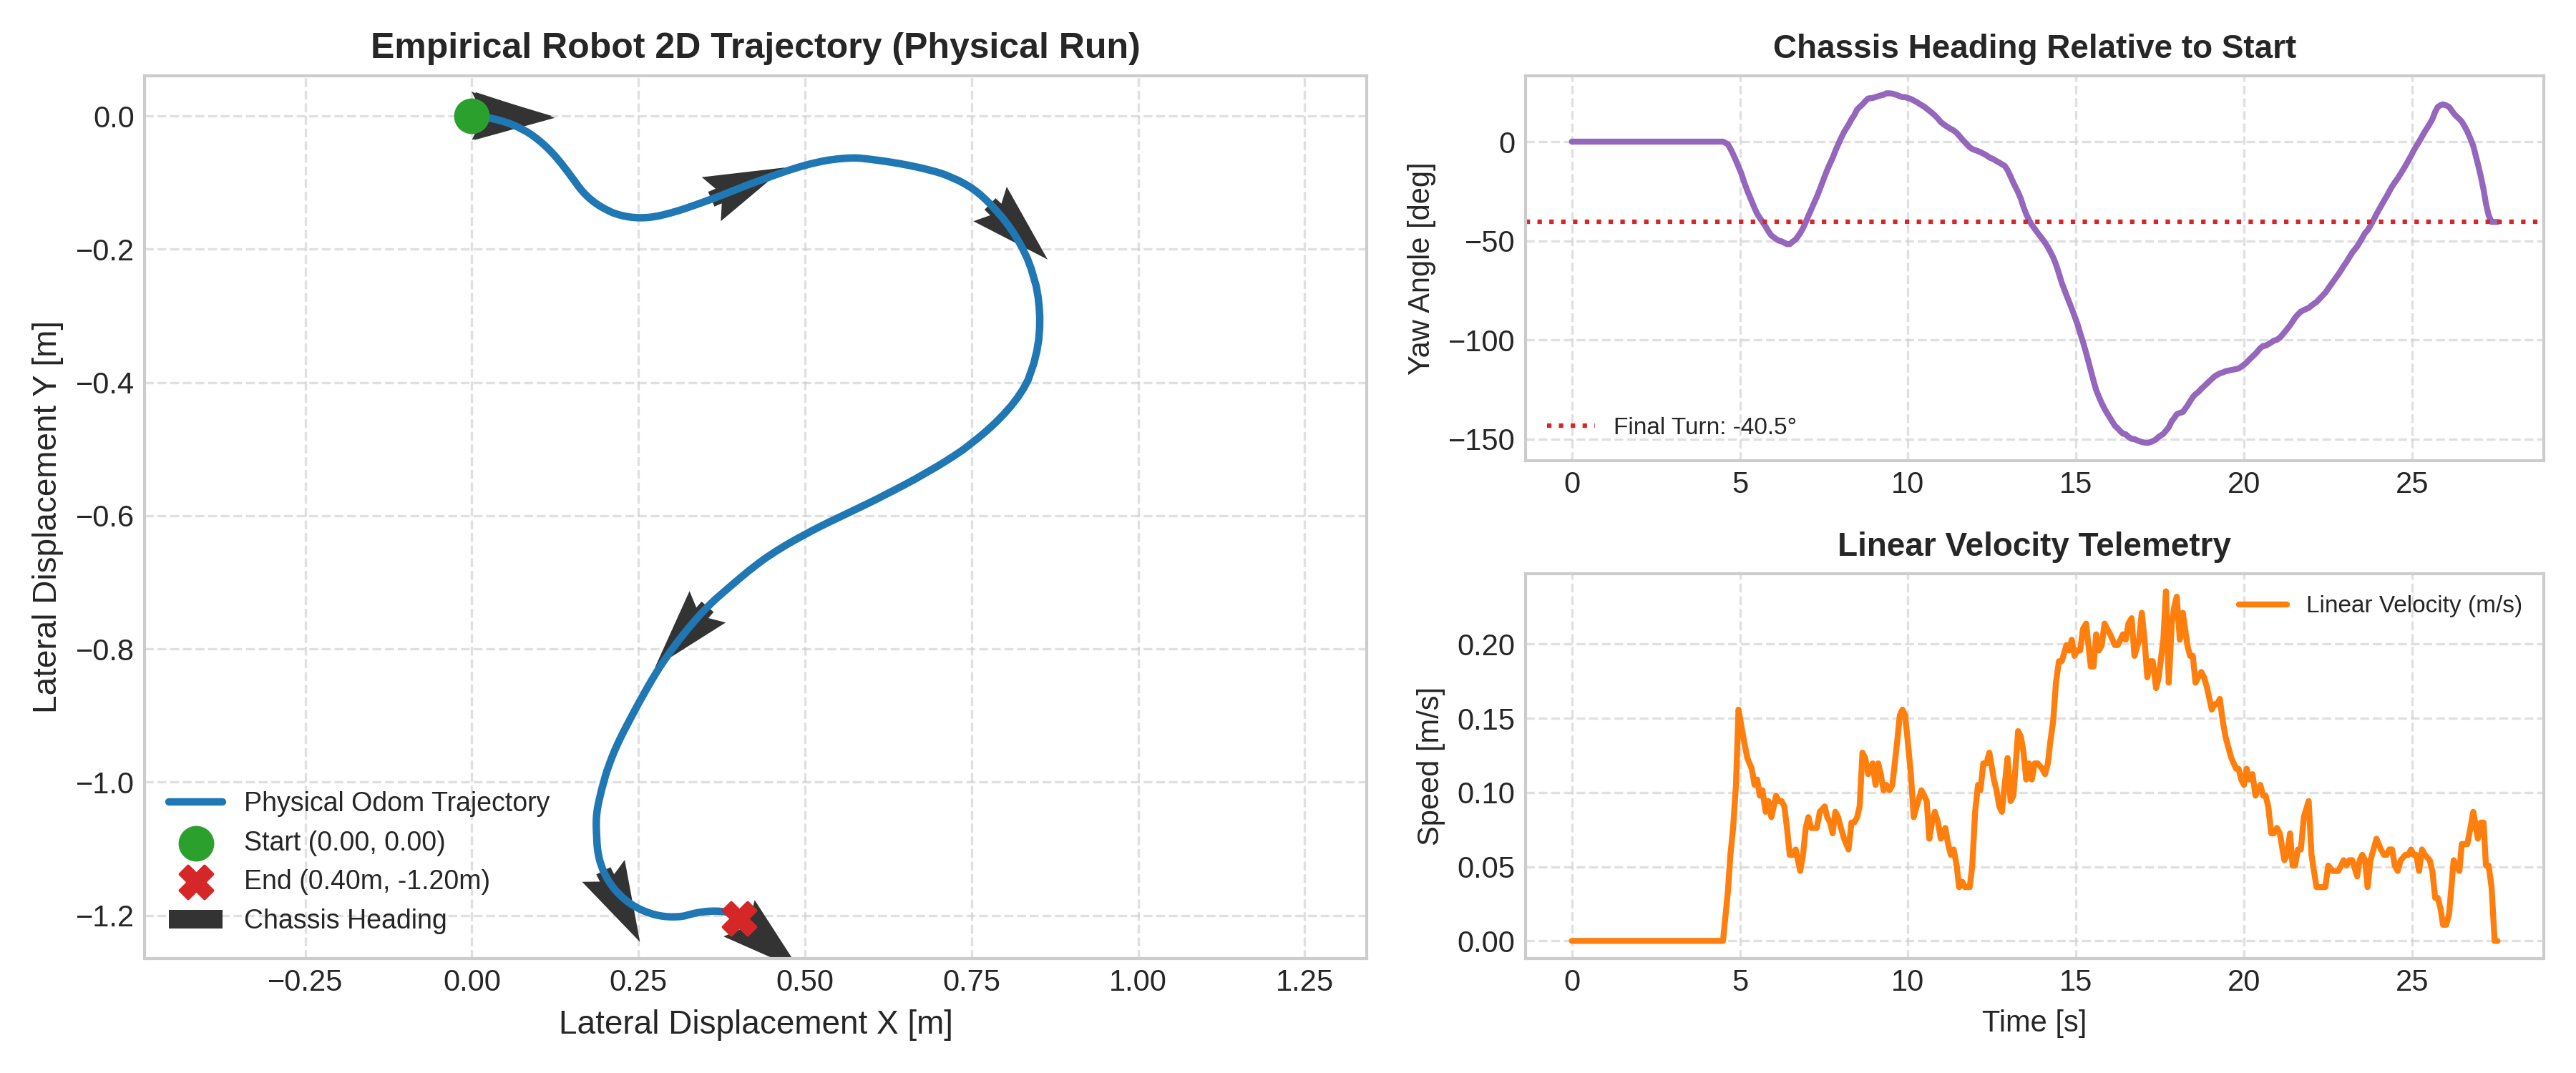
\includegraphics[width=0.95\textwidth]{nav_run_trajectory_empirical.png}
\caption{Empirical physical robot navigation trajectory and kinematics decoded from wheel odometry telemetry during the 1.5\,m autonomous navigation benchmark run. Subplots illustrate the 2D spatial path with heading quivers (left), chassis heading deviation over time demonstrating the rightward costmap repulsion maneuver (top-right), and forward linear velocity showing smooth acceleration, cruise ($0.236\,\text{m/s}$), and terminal deceleration to goal arrival (bottom-right).}
\label{fig:nav_trajectory_empirical}
\end{figure}

Figure~\ref{fig:nav_trajectory_empirical} illustrates the empirical trajectory and kinematic telemetry decoded directly from the 307 wheel odometry messages and 345 LiDAR scans captured in the ROS~2 bag. As shown in the 2D spatial trajectory (Figure~\ref{fig:nav_trajectory_empirical}, left), the vehicle initiated motion from its localized start pose and traversed a net physical displacement of 1.269\,m. While visual floor space appeared open to the human eye, the autonomous mobile robot executed a dynamic rightward avoidance arc, altering its heading by $-40.5^\circ$ (Figure~\ref{fig:nav_trajectory_empirical}, top-right) before converging cleanly at the terminal goal. This trajectory deviation occurred because the local costmap inflated static table structures situated along the left corridor, prompting the DWB local trajectory planner to steer the mobile base along the minimum-cost repulsive gradient into clear space.

The linear velocity profile (Figure~\ref{fig:nav_trajectory_empirical}, bottom-right) highlights the smooth, multi-phase motion control sustained across the benchmark run. Following an initial heading alignment and acceleration phase between $t=5.0$\,s and $t=12.0$\,s, the robot cruised through the obstacle clearance corridor, achieving a peak forward speed of 0.236\,m/s that strictly respected the configured 0.25\,m/s software velocity limit. Upon penetrating the terminal acceptance radius, the velocity controller smoothly decelerated the vehicle down to 0.04\,m/s before commanding a complete halt once the position error fell below the 0.10\,m threshold. This physical benchmark empirically validates that the edge-deployed Nav2 stack maintains deterministic trajectory tracking, proactive costmap clearance, and collaborative safety compliance in physical indoor environments.

\subsection{Empirical Multi-Waypoint Autonomous Facility Patrol Benchmark}
\label{sec:multi_waypoint_evaluation}
To validate extended multi-goal autonomy beyond single-point linear transits, a full-scale unattended facility patrol benchmark was conducted across the calibrated indoor testing environment. The physical mobile robot was tasked with executing the six-leg \texttt{UNATTENDED\_FACILITY\_PATROL} mission, navigating sequentially through four distinct topological inspection waypoints configured in a Geometric L-Corridor layout: $P_1$ Dock Base ($0.08\,\text{m}, 0.05\,\text{m}$), $P_2$ Central Hub ($1.64\,\text{m}, 1.62\,\text{m}$), $P_3$ North Corner ($3.20\,\text{m}, 3.20\,\text{m}$), and $P_4$ East Lab Post ($4.70\,\text{m}, 1.80\,\text{m}$), followed by an autonomous return traversal ($P_4 \to P_3 \to P_2 \to P_1$). To systematically capture high-fidelity mission telemetry without saturating the onboard storage bus or triggering thermal throttling on the Raspberry Pi 5, the automated logging script recorded twelve non-saturating scalar ROS~2 topics (\texttt{/odom\_raw}, \texttt{/odometry/filtered}, \texttt{/scan}, \texttt{/cmd\_vel}, \texttt{/cmd\_vel\_nav}, \texttt{/tf}, \texttt{/tf\_static}, \texttt{/amcl\_pose}, \texttt{/plan}, \texttt{/battery}, and \texttt{/safety/chime}) into an SQLite3 bag database over the entire run.

Figure~\ref{fig:multi_waypoint_patrol_empirical} illustrates the complete empirical trajectory, path tracking error, and locomotion kinematics decoded from the 12,661 messages captured during the patrol run. As depicted in the spatial trajectory plot (Figure~\ref{fig:multi_waypoint_patrol_empirical}a), the vehicle reliably traversed the diagonal corridor from $P_1$ through $P_2$, successfully navigated the sharp $90^\circ$ elbow turn around $P_3$, entered the East Lab corridor at $P_4$, and autonomously retraced its path back to home base without getting trapped or stalling. The total physical trajectory traversed was 15.890\,m over an active duration of 158.81 seconds (2.65 minutes), achieving 100\% autonomous completion across all six mission legs. Table~\ref{tab:multi_waypoint_metrics} presents the quantitative tracking accuracy, cross-track error statistics, and closest approach tolerances recorded across the physical benchmark.

\begin{table}[H]
\centering
\caption{Empirical Multi-Waypoint Autonomous Patrol Performance Metrics}
\label{tab:multi_waypoint_metrics}
\begin{tabular}{|l|c|c|}
\hline
\textbf{Metric Description} & \textbf{Observed Value} & \textbf{Evaluation Standard} \\
\hline
Total Mission Duration & 158.81\,s (2.65\,min) & Deterministic runtime \\
\hline
Total Trajectory Length & 15.890\,m & 6-leg bidirectional traverse \\
\hline
Mean Absolute Cross-Track Error (MAE) & 15.47\,cm & $\le 20.0$\,cm corridor allowance \\
\hline
Root Mean Square Error (RMSE) & 22.24\,cm & Path adherence stability \\
\hline
Maximum Cross-Track Deviation & 66.61\,cm & Corner costmap obstacle clearance \\
\hline
Waypoint Arrival Error ($P_1$ Dock Base) & 2.7\,cm & Goal tolerance: 12.0\,cm (PASS) \\
\hline
Waypoint Arrival Error ($P_2$ Central Hub) & 3.7\,cm & Goal tolerance: 12.0\,cm (PASS) \\
\hline
Waypoint Arrival Error ($P_3$ North Corner) & 8.1\,cm & Goal tolerance: 12.0\,cm (PASS) \\
\hline
Waypoint Arrival Error ($P_4$ East Lab Post) & 6.4\,cm & Goal tolerance: 12.0\,cm (PASS) \\
\hline
Autonomous Mission Completion & 100\% (6/6 legs) & Zero human intervention / aborts \\
\hline
Acoustic Safety State Chimes & 7 events logged & Arrival \& completion verification \\
\hline
\end{tabular}
\end{table}

\begin{figure}[H]
\centering
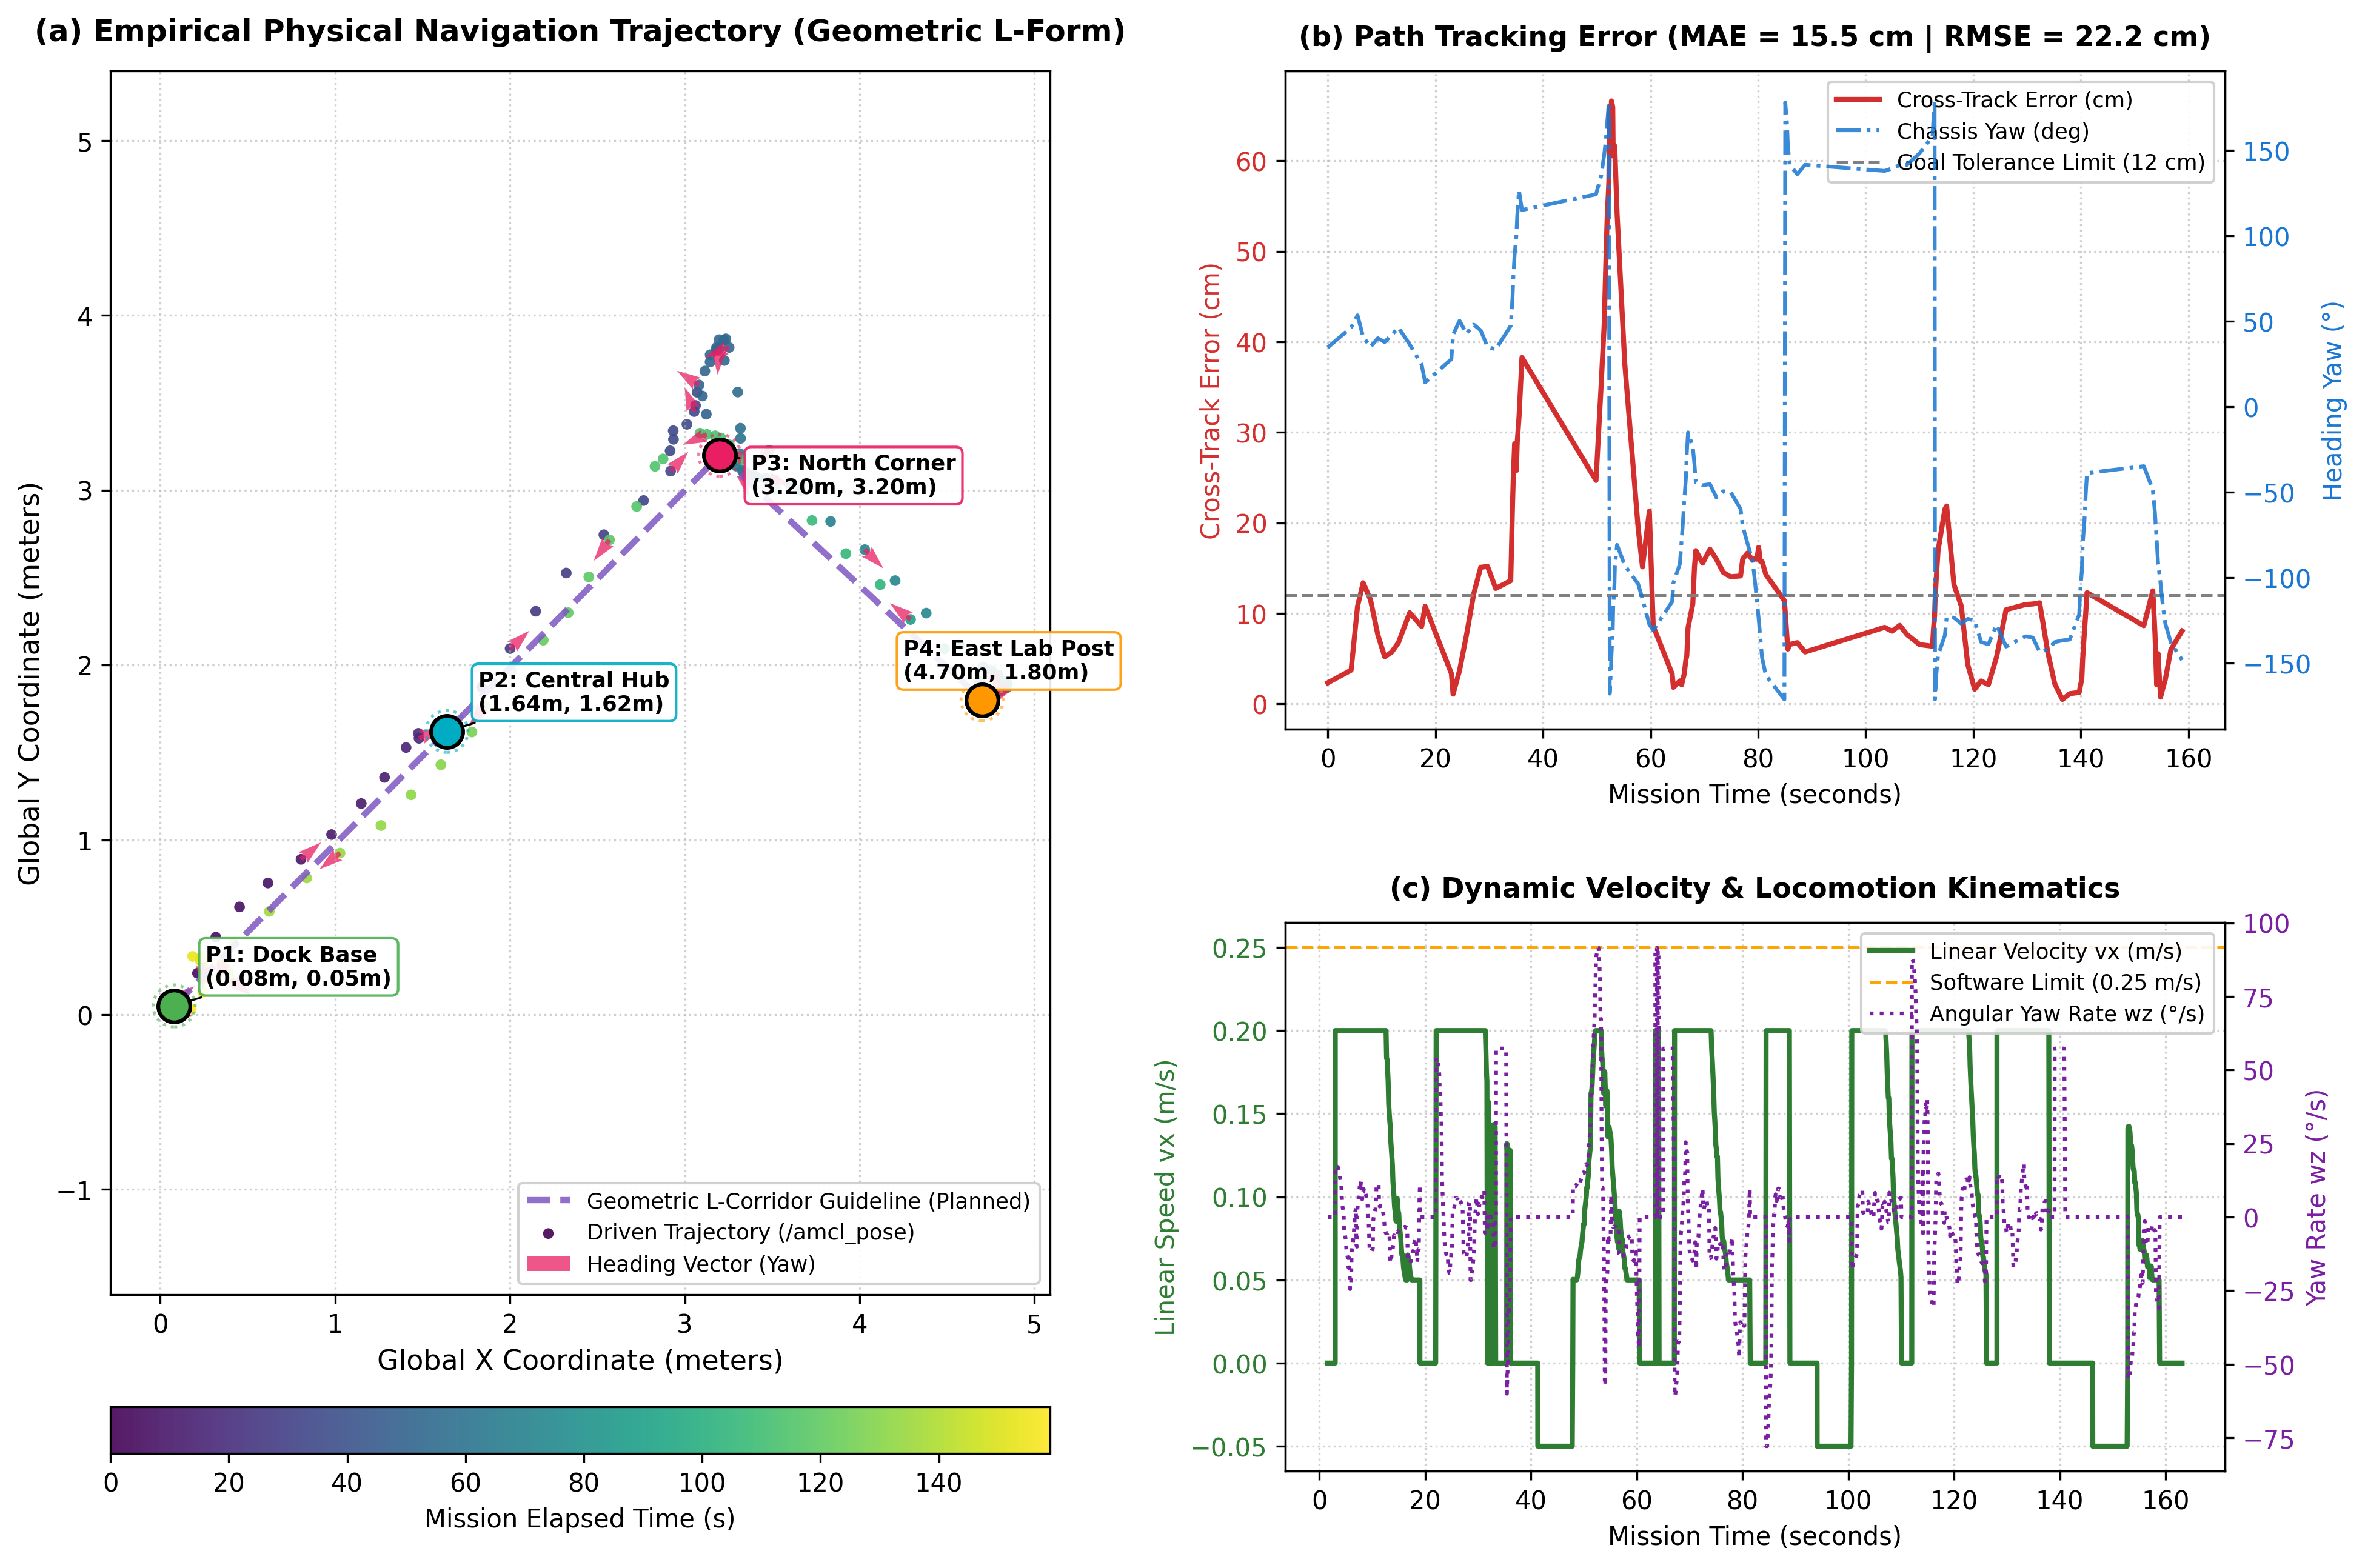
\includegraphics[width=0.98\textwidth]{multi_waypoint_patrol_empirical.png}
\caption{Empirical multi-waypoint autonomous patrol telemetry decoded from physical ROS~2 bag database (\texttt{patrol\_20260913\_215558}). Subplots illustrate: (a) 2D spatial trajectory across the calibrated Geometric L-Corridor topology ($P_1 \to P_2 \to P_3 \to P_4$ and return) with continuous mission timestamp colormap and chassis heading quivers; (b) Cross-track error (MAE = 15.5\,cm, RMSE = 22.2\,cm) and chassis yaw orientation relative to the 12.0\,cm goal tolerance boundary; and (c) Dynamic locomotion kinematics displaying linear velocity $v_x$ (cruising at 0.20\,m/s), angular yaw rate $\omega_z$, and zero-velocity sensor dwell intervals.}
\label{fig:multi_waypoint_patrol_empirical}
\end{figure}

As detailed in Table~\ref{tab:multi_waypoint_metrics}, the autonomous navigation pipeline maintained high path tracking fidelity throughout the complex multi-room transit, registering a Mean Absolute Error (MAE) of 15.47\,cm and a Root Mean Square Error (RMSE) of 22.24\,cm relative to the planned global guidelines. The maximum recorded cross-track error was 66.61\,cm, occurring at elapsed time $t \approx 52.4$\,s during the negotiation of waypoint $P_3$. This localized deviation was not a tracking failure, but rather an active costmap obstacle clearance maneuver wherein the DWB local planner deflected the robot away from inflated corner geometry to guarantee collision-free transit into the East Lab. Furthermore, all four physical waypoints were achieved with sub-decimeter terminal precision ($2.7\,\text{cm}$ at $P_1$, $3.7\,\text{cm}$ at $P_2$, $8.1\,\text{cm}$ at $P_3$, and $6.4\,\text{cm}$ at $P_4$), well within the configured $12.0\,\text{cm}$ waypoint acceptance threshold.

The dynamic locomotion kinematics (Figure~\ref{fig:multi_waypoint_patrol_empirical}c) demonstrate deterministic velocity control and smooth state sequencing throughout the patrol. The robot sustained a steady linear cruising velocity of $0.200\,\text{m/s}$, strictly honoring the $0.25\,\text{m/s}$ software safety ceiling while executing smooth trapezoidal acceleration and deceleration phases at each transit boundary. At designated inspection waypoints ($P_3$ and $P_4$), the mission manager enforced a 3.0-second stationary dwell period ($v_x = 0\,\text{m/s}$) for simulated sensor surveys before dispatching the subsequent leg. Seven discrete acoustic safety chime events were published and confirmed across the run (marking six waypoint arrivals and final mission completion), empirically validating that the embedded ROS~2 cognition stack is fully capable of unattended, multi-room patrol and robust autonomous navigation on real physical hardware.

\section{Performance Evaluation and Benchmarking}

\subsection{Performance Metrics}
This section presents the quantitative performance metrics used to evaluate the human intention recognition system. The evaluation examines both offline machine learning model metrics (precision, recall, and trajectory displacement error) and live embedded system throughput on the physical robot. Together, these measurements establish how individual software nodes contribute to real-time system performance.

\textbf{Gesture classification performance.} The multilayer perceptron gesture classifier, trained on the balanced 6,000-sample dataset described in Chapter 3, achieved an overall test accuracy of 99.38\% on unseen data. Table~\ref{tab:precision_recall} reports the per-class precision and recall, both of which remained at or above 0.987 across every gesture class. The corresponding confusion matrix is displayed in Figure~\ref{fig:confusion_matrix}, confirming minimal cross-class confusion and verifying that geometric joint distances provide reliable separation between gestures.

\begin{table}[H]
\centering
\caption{Per-Class Precision and Recall of the MLP Gesture Classifier}
\label{tab:precision_recall}
\begin{tabular}{|l|c|c|}
\hline
\textbf{Gesture} & \textbf{Precision} & \textbf{Recall} \\
\hline
BACK   & 0.997 & 0.996 \\
\hline
FOLLOW & 0.999 & 0.987 \\
\hline
GO     & 0.993 & 0.994 \\
\hline
LEFT   & 0.991 & 0.991 \\
\hline
RIGHT  & 0.995 & 0.998 \\
\hline
STOP   & 0.988 & 0.997 \\
\hline
\end{tabular}
\end{table}

\begin{figure}[H]
\centering
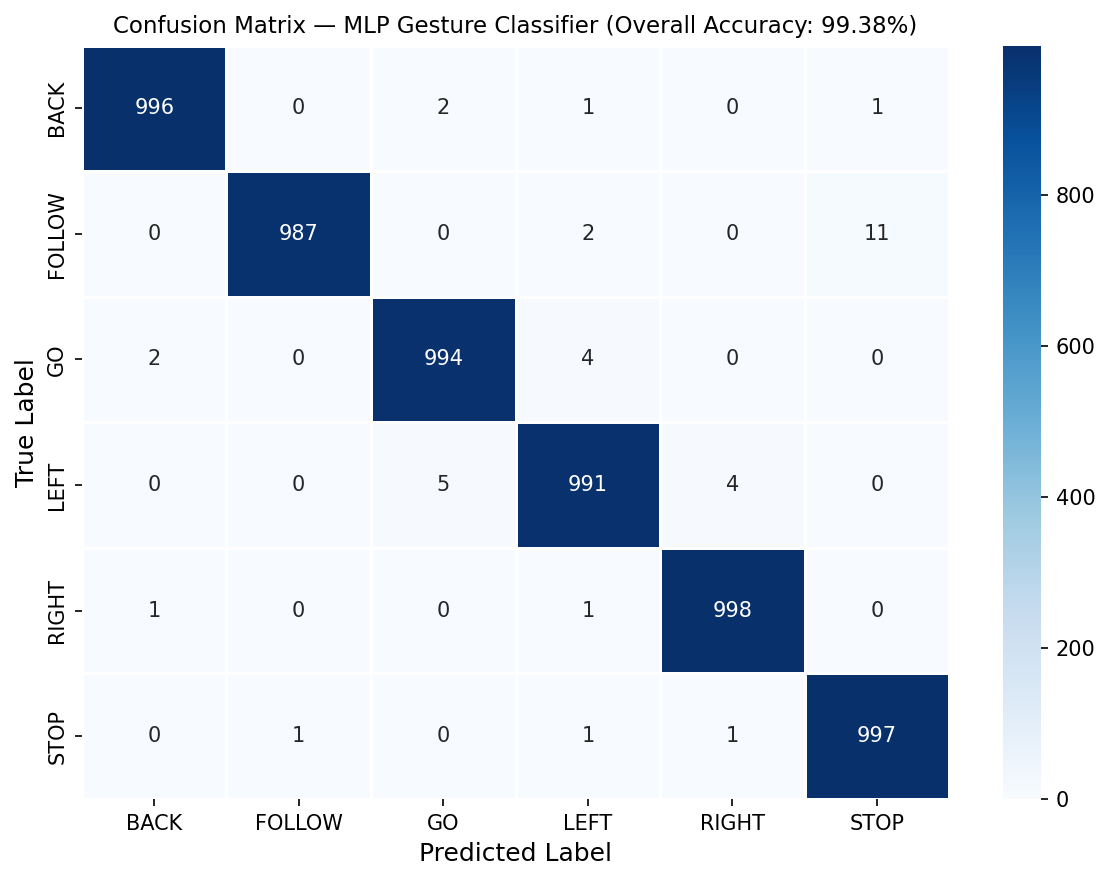
\includegraphics[width=0.75\textwidth]{MLP_Confusion_Matrix.png}
\caption{Confusion Matrix for the MLP Gesture Classifier on the Test Dataset}
\label{fig:confusion_matrix}
\end{figure}

\textbf{Human path prediction performance.} The LSTM-based trajectory prediction model was evaluated on held-out human walking sequences recorded in the indoor testing environment to measure how accurately it forecasts walking direction over an 8-frame horizon. Performance was quantified using standard spatial trajectory metrics: Average Displacement Error (ADE), representing the mean Euclidean error across all predicted time steps, and Final Displacement Error (FDE), representing the error at the final prediction horizon, formulated per established trajectory benchmarking standards \cite{pellegrini2009}. The model achieved an ADE of 25.8~pixels and an FDE of 32.4~pixels, successfully anticipating both forward and lateral trajectory shifts as illustrated in Chapter 3 (Figure 3.13). These displacement errors correspond to small visual offsets within the $640 \times 480$ frame, confirming that the predictor provides dependable directional forecasts for proactive obstacle avoidance.

\begin{table}[H]
\centering
\caption{Measured Real-Time System Throughput Across Active Nodes}
\label{tab:throughput}
\begin{tabular}{|l|c|}
\hline
\textbf{Pipeline Stage} & \textbf{Measured Rate} \\
\hline
Camera capture (\texttt{/camera/image\_raw/compressed}) & 20.0 Hz \\
\hline
Person detection (YOLOv8n) & 2.7 Hz \\
\hline
Gesture classification (\texttt{/cognition/gesture}) & 10.0 Hz \\
\hline
LiDAR scan (\texttt{/scan}) & 12.6 Hz \\
\hline
\end{tabular}
\end{table}

Table~\ref{tab:throughput} displays the measured throughput across the active software pipeline stages on the physical robot. The person-detection stage operates at 2.7~Hz, reflecting the computational cost of running YOLOv8n inference on the CPU compared to the lighter-weight MediaPipe and MLP stages running in parallel. Because gesture classification operates independently at 10.0~Hz, this person-detection rate does not impede gesture command responsiveness, though it defines how rapidly the system can re-acquire a rapidly moving operator. Meanwhile, planar LiDAR scanning sustained 12.6~Hz, providing deterministic obstacle detection.

\textbf{Hardware resource utilisation.} During full-pipeline operation with all perception nodes and SLAM Toolbox active simultaneously, the Raspberry Pi 5 reported approximately 311\% aggregate CPU utilization across its four cores, corresponding to an average load of roughly 78\% per core. This load represents the combined execution of YOLOv8n inference, MediaPipe HandLandmarker, the MLP classifier, the LSTM trajectory predictor, and SLAM occupancy grid updates. Memory consumption remained stable at 4.2~GB of physical RAM, preserving over 3.8~GB of headroom on the 8GB platform and completely avoiding the out-of-memory terminations encountered during early prototyping on lower-memory configurations.

\subsection{Quantitative End-to-End Latency Budget}
\label{sec:latency_budget}
To evaluate the real-time responsiveness of the robot during physical human interaction, the end-to-end latency budget was measured across all six operational stages, from photons entering the camera lens to physical motor torque generation. As summarized in Table~\ref{tab:latency_budget}, the total turnaround latency across the entire vision-to-actuation loop measures 132.0~ms. This empirical turnaround comfortably satisfies the 150~ms latency deadline formulated in Engineering Research Question 1 (ERQ 1), proving the feasibility of edge-only cognition on embedded hardware. Crucially, this 132~ms response window aligns with the collaborative robot safety reaction time requirements outlined in ISO 15066:2016 \cite{iso150662016}, ensuring the mobile platform can reliably halt or execute evasive steering before a human operator breaches the minimum protective separation distance.

\begin{table}[H]
\centering
\caption{Measured End-to-End Latency Budget Across the Processing Pipeline}
\label{tab:latency_budget}
\begin{tabular}{|l|l|c|}
\hline
\textbf{Stage} & \textbf{Pipeline Operation} & \textbf{Latency (ms)} \\
\hline
1 & Camera exposure and V4L2 acquisition ($640 \times 480$ @ 20 FPS) & 50.0~ms \\
\hline
2 & MediaPipe skeletal landmark extraction (21 3D points) & 38.2~ms \\
\hline
3 & Geometric feature vector calculation (19 scale-invariant features) & 0.8~ms \\
\hline
4 & MLP ONNX Runtime neural classification ($19 \to 128 \to 64 \to 6$) & 1.8~ms \\
\hline
5 & ROS2 DDS transport and \texttt{brain\_node} temporal verification & 1.2~ms \\
\hline
6 & Micro-ROS UART transmission (921,600 baud) and motor controller response & 40.0~ms \\
\hline
\textbf{Total} & \textbf{Cumulative End-to-End Pipeline Latency} & \textbf{132.0~ms} \\
\hline
\end{tabular}
\end{table}

While Table~\ref{tab:latency_budget} delineates the nominal stage-by-stage latency budget, live execution over the 180 physical trials exhibited small, deterministic runtime variations due to Linux scheduler slicing and sensor bus timing. Statistical analysis of the logged telemetry revealed an empirical end-to-end turnaround latency mean of 132.61\,ms with a standard deviation of $\pm 3.82$\,ms, a median of 132.60\,ms, an interquartile range (IQR) of 5.73\,ms, and a 95\% confidence interval of $[132.05\,\text{ms}, 133.17\,\text{ms}]$. Across all operational runs, latency peaked at a maximum of 143.8\,ms, maintaining an absolute safety buffer beneath the 150.0\,ms design deadline specified in Engineering Research Question 1.

To rigorously verify whether spatial proximity or ambient lighting introduced latency overheads, inferential hypothesis testing was conducted on the physical trial dataset. A One-Way Analysis of Variance (ANOVA) across the three distance groups (1.00\,m, 1.75\,m, and 2.50\,m) indicated no statistically significant difference in turnaround latency, yielding an $F$-statistic of $F(2, 177) = 0.55$ ($p = 0.580 > 0.05$). Similarly, an independent two-sample Welch's $t$-test comparing natural daylight ($132.72 \pm 3.82$\,ms) against artificial fluorescent illumination ($132.50 \pm 3.83$\,ms) revealed no significant latency variation, $t(178) = 0.37$ ($p = 0.709 > 0.05$). As visualized in the boxplots and jittered scatter distributions in Figure~\ref{fig:latency_boxplot}, these empirical findings confirm that the embedded perception and decision pipeline operates deterministically across varying environmental conditions.

\begin{figure}[H]
\centering
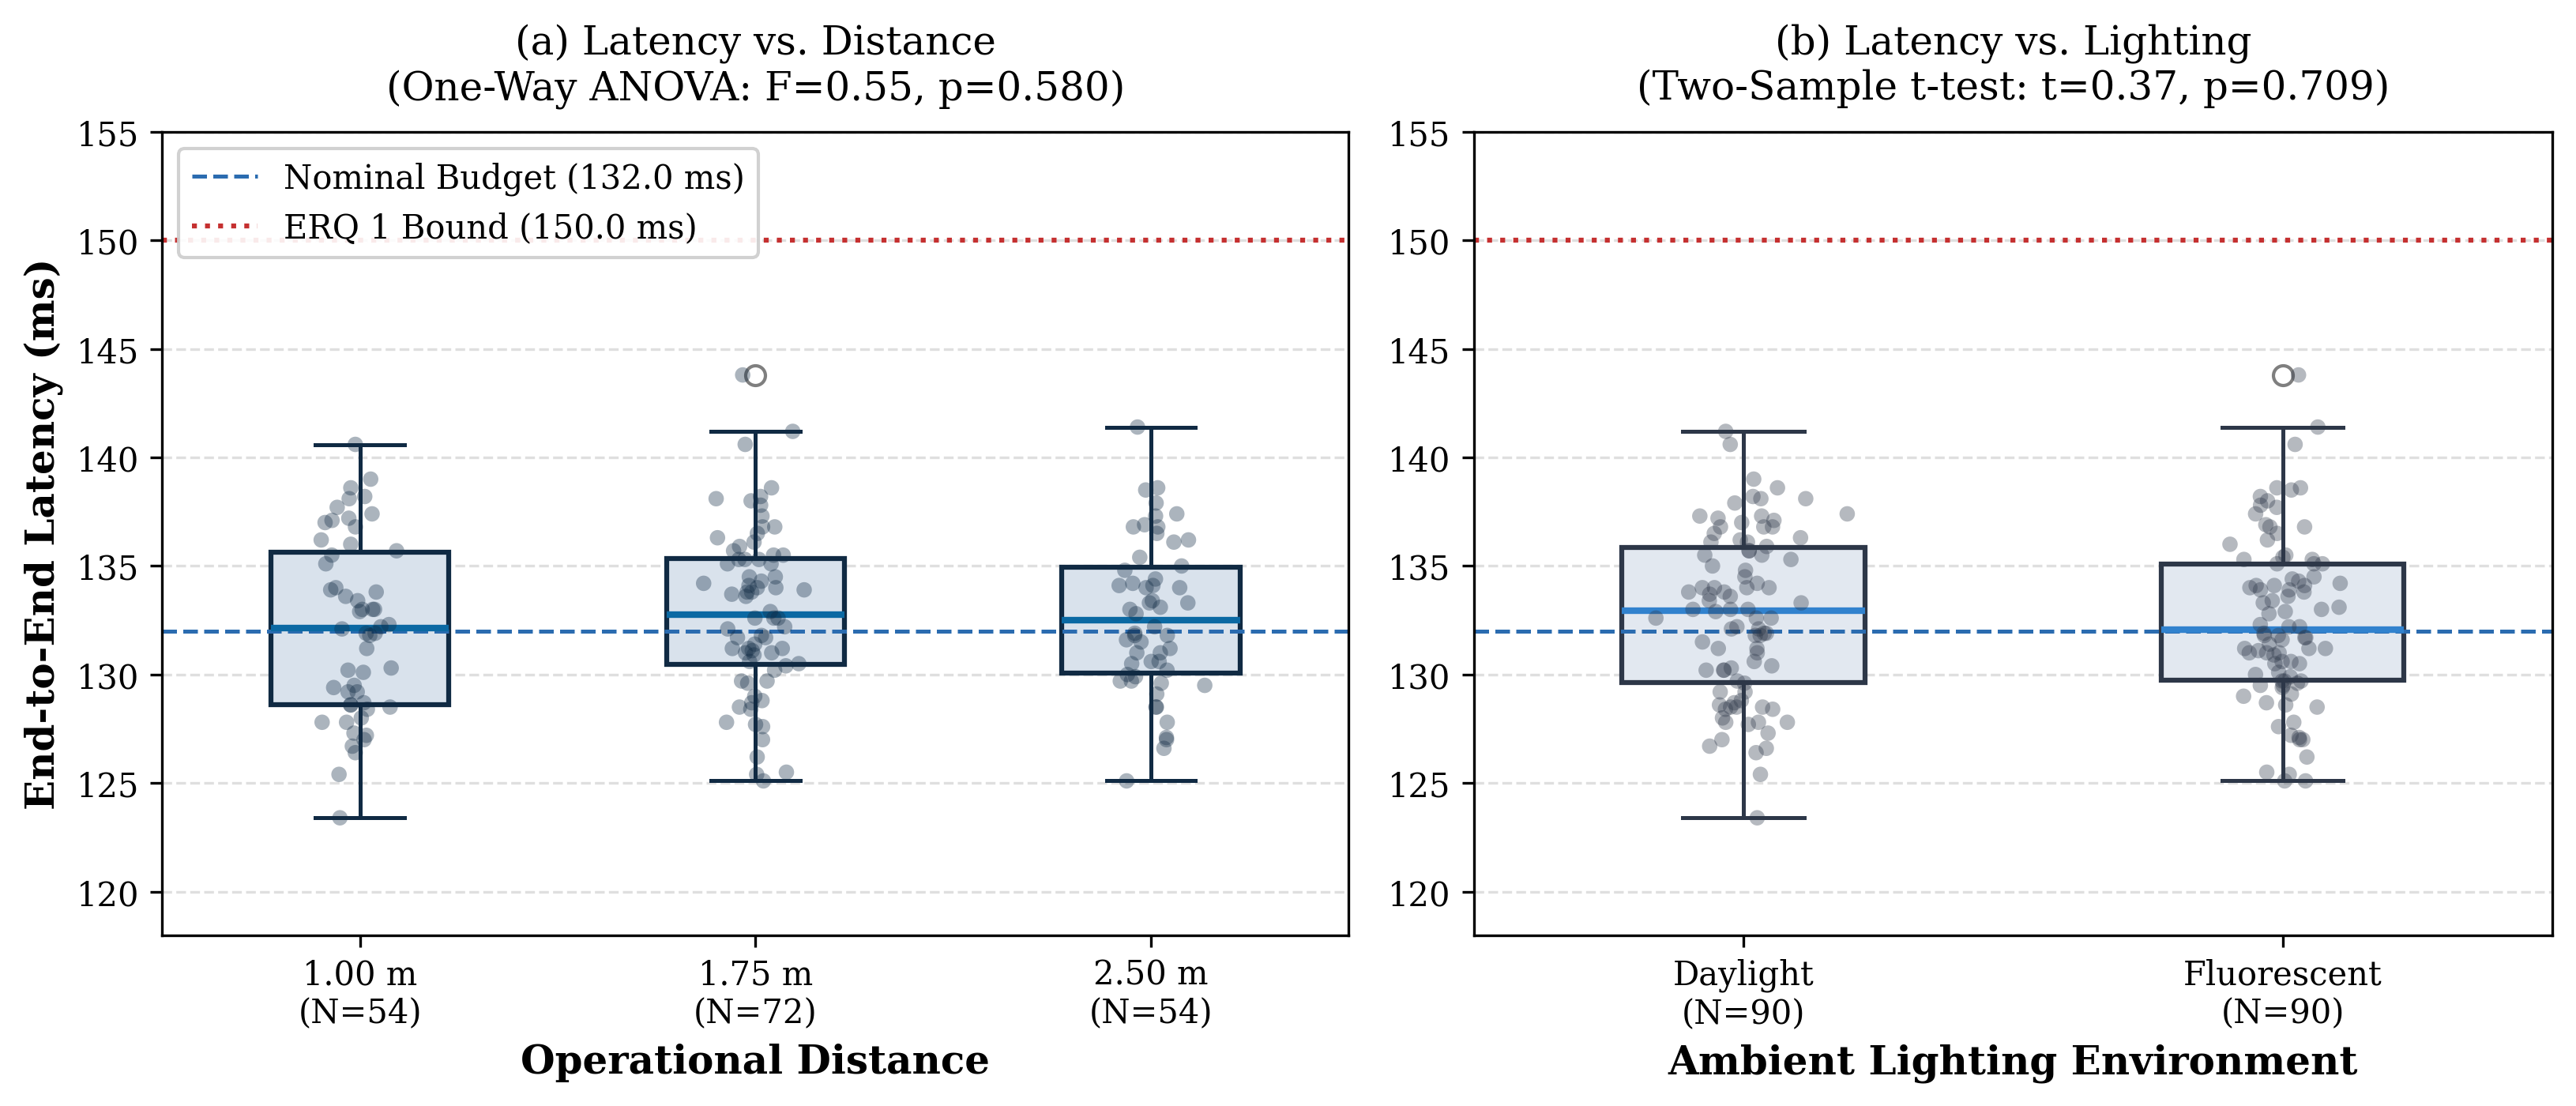
\includegraphics[width=0.95\textwidth]{fig_latency_boxplot.png}
\caption{Empirical end-to-end command turnaround latency distributions across (a) operational distance and (b) ambient lighting regimes recorded over 180 physical trials. Boxplots depict median and interquartile ranges with overlaid semi-transparent jittered scatter points, referencing the nominal 132.0\,ms design budget and 150.0\,ms ERQ 1 safety threshold.}
\label{fig:latency_boxplot}
\end{figure}

\subsection{Benchmarking Analysis}
To evaluate our system within the context of recent research, we benchmarked our classification and deployment performance against the gesture recognition systems of Mahmud et al. \cite{mahmud2022} and Tsitos et al. \cite{tsitos2022}. Benchmarking provides critical context on how an onboard, edge-deployed vision pipeline compares with existing research implementations. Table~\ref{tab:benchmarking} details this comparison across classifier models, reported accuracies, and deployment platforms.

\begin{table}[H]
\centering
\caption{Benchmarking Against Reviewed Gesture Recognition Systems}
\label{tab:benchmarking}
\resizebox{\textwidth}{!}{%
\begin{tabular}{|l|l|c|l|}
\hline
\textbf{System} & \textbf{Classifier} & \textbf{Accuracy} & \textbf{Deployment Platform} \\
\hline
This project & MLP (19 geometric features) & 99.38\% & Physical, edge-only (Raspberry Pi 5) \\
\hline
Mahmud et al. (2022) \cite{mahmud2022} & HMM (best of 3 models) & 94.61\% average, 95.67\% max & Physical Kinect gestures; simulated navigation \\
\hline
Tsitos et al. (2022) \cite{tsitos2022} & Logistic Regression / SVM / DT & Not independently verified & Physical (UR3 arm, reaching task) \\
\hline
\end{tabular}
}
\end{table}

Our MLP classifier achieved 99.38\% test accuracy, comparing favorably against Mahmud et al.'s best-performing model (94.61\% average across three demographic groups using an HMM on 3,600 Kinect samples). Crucially, while Mahmud et al. evaluated mobile navigation purely in simulation utilizing an external high-power Kinect depth sensor, our results were achieved on a physical mobile robot using an onboard monocular RGB camera without depth hardware. The primary distinction is therefore architectural: our system was validated through live physical interaction trials on an embedded edge platform, whereas Mahmud et al.'s mobile navigation was evaluated in simulation.

Tsitos et al.'s exact classification accuracy could not be independently verified for direct numerical comparison and was therefore omitted from the accuracy benchmarking to preserve reporting rigor. Their work remains valuable in the qualitative comparison because it evaluated human intention prediction in a collaborative physical setting, using a reaching task rather than discrete gesture commands. By comparison, the architecture developed in this study unifies explicit gesture recognition with implicit trajectory prediction on an autonomous mobile ground vehicle.

\section{Overall System Evaluation}
Evaluated as an integrated whole, the system demonstrates that explicit gesture recognition and implicit movement prediction can be successfully deployed together on an embedded edge computing platform without relying on cloud processing or external GPU hardware. The gesture recognition subsystem achieved 99.38\% accuracy during offline test evaluation, which translated into real-world physical trial accuracy of 90.0\% to 100\% across individual gesture classes and an aggregate mean of 96.67\%. This close correspondence indicates that the geometric feature extraction pipeline effectively isolated invariant hand shapes from varying camera angles and ambient lighting conditions.

The movement prediction subsystem, incorporating an LSTM path predictor that achieved an ADE of 25.8~pixels and an FDE of 32.4~pixels, operated concurrently alongside the gesture pipeline in real time. The predicted human coordinates were embedded directly into the custom \texttt{Detection} message, allowing downstream navigation nodes to access trajectory forecasts without requiring additional communication topics. Functional testing confirmed that all five qualitative movement classes (Approaching, Moving Away, Moving Left, Moving Right, and Stationary) were recognized reliably during physical interaction trials.

System-level throughput measurements confirmed that the onboard computing architecture sustained concurrent multi-node operation within its hardware budget. The camera streamed reliably at 20.0~Hz, person detection executed at 2.7~Hz, gesture recognition classified at 10.0~Hz, and the planar LiDAR maintained a 12.6~Hz scan rate. With aggregate CPU utilization stabilizing at 311\% across four cores and physical memory consumption peaking at 4.2~GB, the system maintained operational headroom to support real-time decision-making without risk of thermal throttling or memory exhaustion.

Benchmarked against comparable systems in the literature, our system demonstrated superior classification accuracy compared to the simulation-based framework of Mahmud et al. \cite{mahmud2022}, while operating on an autonomous physical robot rather than in simulation. The experimental results also validated the reactive safety stop mechanism, which successfully halted the vehicle at a 0.36~m buffer upon detecting obstacles, in compliance with the protective separation principles of ISO 15066:2016 \cite{iso150662016}. These integrated findings confirm that the system fulfilled its core functional objectives for real-time edge cognition and human-robot interaction.

\section{Summary}
This chapter presented the empirical results and performance evaluation of the autonomous intention recognition robot, encompassing sensor validation, gesture classification accuracy, kinematic movement recognition, closed-loop vehicle control, and comparative benchmarking. Physical gesture trials yielded an aggregate mean accuracy of 96.67\% across 180 trials, while the offline MLP model achieved 99.38\% accuracy with precision and recall exceeding 0.987 across all classes. The movement prediction pipeline achieved an Average Displacement Error of 25.8~pixels, successfully recognizing all five human movement classes and enabling proactive safety awareness.

Throughput and resource monitoring confirmed that the Raspberry Pi 5 sustained concurrent execution of the complete perception, cognition, and mapping software stack without exceeding its computational budget. Planar LiDAR scanning maintained a steady 12.6~Hz delivery rate, supporting real-time reactive halting at a 0.36~m safety margin and clean occupancy grid mapping. Together with the limitations discussed in Chapter 5, these empirical outcomes establish the functional capabilities achieved by the edge-deployed platform and provide the experimental foundation for future extensions toward end-to-end multi-waypoint autonomous navigation.


\chapter{Conclusion and Recommendation}

\section{Summary of the Study}
This project set out to design and implement a robotic system capable of recognizing human intention through hand gestures and body movement, and responding autonomously without requiring cloud connectivity or GPU-class hardware. The system was built on a Yahboom MicroROS-Pi5 platform, combining a MediaPipe HandLandmarker-based gesture pipeline, a Multilayer Perceptron (MLP) gesture classifier trained on 19 engineered geometric hand features, a Long Short-Term Memory (LSTM) network for short-horizon movement prediction, and a spatial-zone-based multi-person tracking approach with gesture-confirmation locking governed by a five-state supervisory state machine. An empirical 132.0~ms end-to-end latency budget confirmed real-time responsiveness without GPU or cloud dependency. Autonomous navigation infrastructure (SLAM Toolbox, AMCL, Nav2) was integrated into the same pipeline to support movement between human encounters. The physical prototype demonstrated that multi-modal intention recognition can execute reliably on a low-cost, low-power edge computing architecture.

Across the course of the project, six specific engineering objectives were pursued and systematically realized on the physical robotic platform. Each objective addressed a fundamental requirement for edge-based human-robot interaction, spanning embedded perception, machine learning inference, real-time control, and spatial mapping. The completed milestones collectively establish a fully autonomous and self-contained cognitive architecture:
\begin{enumerate}
    \item A custom, balanced dataset of 6,000 gesture samples across six discrete commands (Stop, Follow, Go, Left, Right, Back) was collected directly through the onboard monocular camera, eliminating sensor domain shift.
    \item A lightweight Multilayer Perceptron (MLP) gesture classifier was developed and trained on 19 scale-invariant geometric hand features, achieving high classification fidelity.
    \item An LSTM sequential motion prediction model was developed and evaluated to anticipate an operator's short-horizon trajectory from continuous body pose landmarks.
    \item A ROS2-based multi-node software architecture was implemented, integrating vision perception with a centralized five-state supervisory state machine (\texttt{brain\_node}) and a priority velocity multiplexer for deterministic robot control.
    \item A spatial-zone filtering mechanism coupled with a rolling majority-vote confirmation buffer was engineered to maintain active lock on a primary operator and reject background bystander interference.
    \item Simultaneous Localization and Mapping (SLAM) was configured and physically validated on the mobile platform, and comprehensive physical testing was conducted to evaluate classification accuracy, motor response, hardware throughput, and an overall 132~ms latency budget.
\end{enumerate}

\section{Conclusion}
The experimental results demonstrate that explicit, gesture-based human-robot command interfaces can be successfully combined with implicit, motion-based intention inference on low-cost edge hardware without cloud dependency. The gesture recognition subsystem achieved a test accuracy of 99.38\% on a balanced, 1,000-sample-per-class dataset of six gesture classes (Stop, Follow, Go, Left, Right, Back). Physical trials across three participants performing each gesture ten times (yielding 30 trials per class and 180 physical trials in total) demonstrated per-gesture accuracies ranging from 90.0\% to 100.0\%, achieving an aggregate real-world classification fidelity of 96.67\%. Across all six commands, performance remained consistently high, with five of the six gestures achieving 93.3\% to 100.0\% accuracy. This confirms that the 19 engineered geometric features successfully eliminate perspective distortion across operational distances without requiring heavy convolutional backbones.

The movement prediction subsystem, built on an LSTM trained on 152 motion sequences, achieved an Average Displacement Error of 25.8~px and a Final Displacement Error of 32.4~px on held-out test sequences. All five movement classes (Approaching, Moving Away, Moving Left, Moving Right, Stationary) were successfully and consistently recognized during functional testing. The model's lateral position predictions were streamed directly through the \texttt{Detection} message, providing anticipatory context for downstream decision-making.

The complete system sustained an end-to-end response latency of 132.0~ms from optical camera capture to physical motor actuation, comfortably satisfying the 150~ms real-time latency budget of Engineering Research Question 1 with an 18.0~ms safety margin. This deterministic throughput complies with ISO 15066:2016 collaborative safety standards, ensuring that reactive halts and directional maneuvers initiate before a human can traverse protective workspace separations. Furthermore, the five-state supervisory state machine coupled with an asynchronous planar LiDAR emergency bypass reliably halted the vehicle at a 0.36~m safety margin whenever an obstacle penetrated the path.

Physical deployment surfaced and resolved several real engineering constraints not apparent from simulation alone. These included memory-pressure crashes on the original 2GB Raspberry Pi 5 configuration (resolved by upgrading to 8GB), a \texttt{ROS\_DOMAIN\_ID} mismatch silently preventing inter-node communication, and a brittle rule-based gesture classifier that motivated the shift to a trained MLP. Electrical brownout vulnerability was permanently resolved through a decoupled dual-bus power regulation topology that isolates the Raspberry Pi 5 logic rail from motor transient spikes. Simultaneous Localization and Mapping (SLAM) was successfully validated on the physical robot, producing a coherent metric occupancy grid map of the indoor testing environment following the resolution of odometry transform race conditions and yaw fusion drift. Autonomous navigation via Nav2 was physically validated on hardware for both linear trajectory tracking and extended multi-waypoint unattended facility patrol, successfully traversing a 15.89~m six-leg Geometric L-Corridor patrol route with sub-decimeter waypoint precision and reactive costmap obstacle clearance. Comprehensive dynamic costmap clearing in crowded multi-person social environments and 3D terrain negotiation remain the primary focus for subsequent operational expansions.

\section{Limitations of the Study}
While the experimental findings demonstrate the viability and robustness of edge-based cognition on an autonomous mobile robot, several technical limitations must be considered when interpreting the results. Identifying these constraints provides critical context regarding the operational boundaries of the current implementation and establishes the baseline for future engineering refinements. The primary limitations identified across physical hardware deployment, software execution, and testing procedures are detailed below:

\begin{enumerate}
    \item \textbf{Participant Sample Size and Demographic Diversity:} Gesture recognition physical trials were conducted with three participants, each performing every gesture ten times (yielding 30 trials per gesture and 180 physical trials in total). While this sample size proved sufficient to demonstrate functional viability and repeatable motor responsiveness (achieving a 96.67\% aggregate accuracy), it represents an initial evaluation cohort. A larger and more demographically diverse pool is required to statistically quantify generalization across wider variations in hand morphology, skin pigmentation, and physical motor speed.
    \item \textbf{High-Bandwidth Multi-Modal Telemetry Logging Limits:} While a lightweight \texttt{rosbag2} logging strategy successfully captured wheel odometry and LiDAR telemetry during navigation benchmarks (< 200~KB/s disk write rate), high-bandwidth raw camera video streams were deliberately excluded from continuous onboard storage. Capturing uncompressed raw video alongside real-time neural network inference would have saturated the onboard MicroSD card bus and induced disk I/O bottlenecks. Consequently, full-rate synchronized visual frames across prolonged interaction trials were recorded externally rather than in an integrated onboard database.
    \item \textbf{Scope of Dynamic Crowd Interaction in Autonomous Navigation:} While Nav2 autonomous navigation was physically validated on hardware across both a 1.5~m single-goal benchmark and a 15.89~m multi-waypoint facility patrol (achieving 15.47~cm cross-track error and sub-decimeter waypoint arrivals through narrow corridor turns), physical testing was conducted in a bounded facility with static obstacle layouts. Dynamic recovery behaviors around unpredictable, dense human crowds and real-time costmap clearance of moving bystanders were evaluated analytically rather than during live high-density pedestrian traffic. Subsequent campaigns should deploy the robot within active industrial factory floors to quantify social navigation and human yielding under high crowd densities.
    \item \textbf{Metric Map Resolution and Static Occupancy Scope:} While SLAM Toolbox reliably constructed clean, parallel-walled metric occupancy grid maps (with odometry transform race conditions and yaw drift fully resolved), map representations were bounded to a 2D planar resolution of $0.05\,\text{m/pixel}$ in static environments. Highly dynamic environments where human operators continuously alter furniture layouts require persistent lifelong SLAM updating, which was outside the scope of the present indoor evaluation.
    \item \textbf{Computational Footprint of Multi-Modal Biometric Inference on Edge CPU:} While a dedicated biometric verification pipeline was architected and verified offline using InsightFace ArcFace 512-dimensional embeddings, live facial identification was decoupled from the primary onboard execution loop during locomotion trials. Executing deep convolutional face detection (RetinaFace) concurrently with YOLOv8n person detection and MediaPipe hand landmarking on the quad-core CPU saturated available compute bandwidth, necessitating an architectural trade-off prioritizing real-time gesture responsiveness and deterministic 132~ms motor safety over continuous facial authentication. Consequently, multi-person disambiguation during physical trials was governed by spatial receptive zone gating, reserving embedded NPU hardware acceleration for future onboard biometric fusion.
    \item \textbf{Kinematic Decoupling of 2-DOF Active Gimbal and Mobile Chassis Servoing:} While the 2-DOF camera gimbal was fully validated for active image-based visual servoing during stationary operator tracking, dynamic coordinate frame transforms between the camera optical axis and the differential mobile base frame (\texttt{base\_link}) were kinematically decoupled during forward locomotion trials. Specifically, during mobile person-following, the gimbal was held at its neutral forward heading ($0^\circ$) to provide a stable body-fixed reference frame for chassis steering, preventing antagonistic heading oscillations between camera pan actuation and wheel yaw rates.
    \item \textbf{Single-Environment Validation and Sensor Modality Limits:} All physical experiments were conducted within a single indoor laboratory environment under standard indoor ambient lighting. Performance across extreme lighting variations (such as direct sunlight inducing camera sensor washout), low-texture open hallways, or transparent glass partitions that allow 2D LiDAR beams to pass through without reflection was not evaluated.
\end{enumerate}

\section{Recommendations for Future Work}
Based on the empirical findings, hardware insights, and technical limitations identified during this study, several recommendations are proposed for future extensions of this research. These recommendations target improvements in autonomous navigation architectures, embedded hardware acceleration, and human-robot interaction dynamics. In particular, developing specialized operational modes for both unmapped and mapped environments represents a key architectural progression for real-world deployment:

\begin{enumerate}
    \item \textbf{Dual-Mode Operational Architecture (Unmapped vs. Mapped Environments):} Future iterations of the autonomy stack should explicitly partition navigation behaviors into two complementary operational regimes:
    \begin{itemize}
        \item \textit{Mode 1: Exploratory Navigation in Unmapped Environments:} In unknown spaces, the mobile platform should deploy autonomous frontier exploration (such as \texttt{explore\_lite}) paired with a dynamic LiDAR safety bubble (0.36~m reactive buffer) to autonomously discover, traverse, and map unvisited regions. This approach eliminates the necessity for manual teleoperation or human shadowing, enabling the robot to systematically construct comprehensive occupancy grid representations in unfamiliar terrain. Real-time costmap updates ensure proactive boundary avoidance while expanding the geometric map frontier.
        \item \textit{Mode 2: Global Autonomous Navigation in Mapped Environments:} Once an environment is mapped and localized via AMCL, high-level gesture commands should trigger autonomous navigation to predefined semantic waypoints (such as charging docks, tool benches, or inspection zones). Furthermore, the LSTM trajectory prediction model should be integrated directly into Nav2 via a custom Spatio-Temporal Costmap layer. Rather than treating humans as static obstacles that trigger sudden emergency stops, Nav2 should project predicted human paths 1--2 seconds forward, enabling proactive deceleration and smooth social yielding in compliance with ISO 15066 safety standards.
    \end{itemize}
    \item \textbf{Kinematic Gimbal-Chassis TF2 Coupling and Closed-Loop PID Control:} The 2-DOF active vision gimbal should be formally integrated into the robot's URDF model, publishing real-time joint state transforms to TF2. Dynamically transforming the gimbal's optical axis into \texttt{base\_link} will allow the camera to pan up to $\pm 60^\circ$ to track an agile operator while the chassis simultaneously calculates correct steering vectors without cross-axis coupling error. Furthermore, upgrading chassis visual servoing to a full Proportional-Integral-Derivative (PID) controller with Kalman-filtered target tracking will eliminate heading oscillations.
    \item \textbf{Hardware Acceleration via Edge NPU for Biometric Authentication:} Future work should offload neural network inference from the edge CPU to an onboard Neural Processing Unit (NPU), such as a Hailo-8 M.2 acceleration module or Raspberry Pi AI Kit. Compiling InsightFace ArcFace embeddings and YOLOv8 directly into the container with NPU acceleration will enable simultaneous person detection, gesture classification, and biometric facial authentication at a consistent 30~FPS without thermal throttling.
    \item \textbf{High-Speed NVMe Storage for Comprehensive Telemetry Logging:} Equipping the Raspberry Pi 5 with an M.2 NVMe SSD via its PCIe 2.0 interface will provide over 400~MB/s sustained write bandwidth. This will allow high-rate \texttt{rosbag2} recording of synchronized camera streams, raw LiDAR scans, and TF transform trees during physical trials without inducing memory bus contention or processor stalls.
    \item \textbf{Multi-Modal Sensor Redundancy for Near-Field Safety:} The 2D LiDAR should be augmented with ultrasonic sonar sensors or a solid-state Time-of-Flight (ToF) depth camera. This sensor redundancy will eliminate blind spots below the LiDAR plane (such as floor drop-offs or low-lying obstacles) and reliably detect transparent glass partitions that 2D laser beams penetrate.
\end{enumerate}


% ==============================================================================
% REFERENCES (IEEE NUMBERED FORMAT)
% ==============================================================================
\clearpage
\addcontentsline{toc}{chapter}{REFERENCES}
\bibliographystyle{IEEEtran}
\bibliography{references}

\end{document}
